% !TeX encoding = UTF-8
% !TeX document-id = {856115b6-76ae-40a0-94c7-827233f04a27}
\documentclass[13pt,a4paper, listof=entryprefix, bibliography=totoc,toc=listofnumbered,lof=listofnumbered]{scrartcl}
																	%toc=listofnumbered
% WICHTIG!!!
% Pseudokommentar um pdflatex zu erlauben andere Programme zu nutzen z.B. gnuplot
% !TeX TXS-program:compile = txs:///pdflatex/[--shell-escape] | txs:///makeindex | txs:///biber | txs:///pdflatex/[--shell-escape]

\usepackage[ngerman]{babel}
\usepackage[utf8]{inputenc}

%Paket fuer einheitlichen Schriftsatz Times Roman
\usepackage{mathptmx}

%Paket wurde eingefügt, damit die Trennung auch bei Umlauten korrekt erfolgt
\usepackage[T1]{fontenc}
%sollte ein Wort trotzdem mal nicht richtig getrennt werden, kann dies durch
%\hyphenation{Durch-füh-rung} %manuel getrennt werden.

\usepackage{amsmath}
\usepackage{booktabs}
\usepackage{nccmath}
\usepackage{amsfonts}
\usepackage{amssymb}
\usepackage{graphicx}
\usepackage{fancyhdr}
\usepackage{geometry}
\usepackage{setspace}
\usepackage[right]{eurosym}
\usepackage{colortbl}
\usepackage{xcolor}
\usepackage{parskip}
\usepackage[pdfpagelabels=true]{hyperref}
\usepackage{listings}
\usepackage{csquotes}
\usepackage{url}
\usepackage{float}
\usepackage{textcomp}
\usepackage{lmodern}
\usepackage{lscape}
\usepackage{verbatim}
\usepackage{enumitem}
\setitemize{leftmargin=*}

% Indizes
\index{Algorithmus -- Pseudocode}
\index{Optimierungsproblem -- Definition}

% Stichwortverzeichnis
\usepackage[nonewpage]{imakeidx}
\makeindex[intoc=false, title=, options=-g -s tex/_index \%.idx]

%-----------------------------------------------------------------------------------
% Bibilothek
%-----------------------------------------------------------------------------------
% Einbinden des BibLateX paketes mit Ausgabeeinstellungen
\usepackage[
style=alphabetic,          % Zitierstil
maxbibnames=50,            % alle Autorennamen anzeigen
maxcitenames=4,            % maximale Namen, die im Kürzel angezeigt werden
autocite=inline,           % regelt Aussehen für \autocite (inline=\parancite)
block=space,               % kleiner horizontaler Platz zwischen den Feldern
backref=false,             % Keine Angaben auf welchen Seiten die Quelle referenziert ist
% backrefstyle=three+,       % fasst Seiten zusammen, z.B. S. 2f, 6ff, 7-10
% date=short,                % Datumsformat
backend = biber,           % Backnend für Aufbereitung
doi=false,                %Keine Ausgabe des DOI
isbn=false                % Keine Ausbage der ISBN
]{biblatex}

%Doppelunkt nach Autorennamen
\renewcommand*{\labelnamepunct}{\addcolon\addspace}

%Zusätzliche für Umbrüche für Kleinbuchstaben z.B. in URLs
\appto\UrlBreaks{\do\a\do\b\do\c\do\d\do\e\do\f\do\g\do\h\do\i\do\j
	\do\k\do\l\do\m\do\n\do\o\do\p\do\q\do\r\do\s\do\t\do\u\do\v\do\w
	\do\x\do\y\do\z}

\newcounter{verzeichnis}
\setcounter{verzeichnis}{1}

%Abstände der Einträge
\setlength{\bibitemsep}{1em}     % Abstand zwischen den Literaturangaben
\setlength{\bibhang}{2em}        % Einzug nach jeweils erster Zeile

% Kürzel soll vier Buchstaben der Autoren enthalten statt drei
\DeclareLabelalphaTemplate{
	\labelelement{
		\field[final]{shorthand}
		\field{label}
		\field[strwidth=4,strside=left,ifnames=1]{labelname}
		\field[strwidth=2,strside=left,ifnames=2]{labelname}
		\field[strwidth=1,strside=left]{labelname}
	}
	\labelelement{
		\field[strwidth=2,strside=right]{year}
	}
}

% Bibliothek der Quellen
\addbibresource{Latex/tex/biblatex.bib}

\makeatletter
\def\input@path{{Latex/}{Latex/tex/}{tex/}}
\makeatother

% --------------------------------------------------------------------------------
% Einstellung für Listings
% --------------------------------------------------------------------------------
\lstset{basicstyle=\footnotesize, captionpos=b, breaklines=true, showstringspaces=false, tabsize=2, frame=lines, numbers=left, numberstyle=\tiny, xleftmargin=2em, framexleftmargin=2em}
\makeatletter
\def\l@lstlisting#1#2{\@dottedtocline{1}{0em}{1em}{\hspace{1,5em} Lst. #1}{#2}}
\makeatother

%Einstellung für Umlaute in Listings
%\lstset{literate=%
%    {Ö}{{\"O}}1
%    {Ä}{{\"A}}1
%    {Ü}{{\"U}}1
%    {ß}{{\ss}}1
%    {ü}{{\"u}}1
%    {ä}{{\"a}}1
%    {ö}{{\"o}}1
%    {~}{{\textasciitilde}}1
%}

%Einstellungen zur Vermeidung von Einrückung bei Aufzählungen
%Aufzählungen mit Punkten
\newenvironment{FHitemize}{\begin{list}{$\bullet$} {\leftmargin1.5em \labelsep1em \rightmargin0cm \parsep0.5ex plus0.2ex minus0.1ex \itemsep0ex plus0.2ex}}{\end{list}}
%Aufzählungen mit Nummerierungen
\setlist[enumerate]{wide=0pt, leftmargin=*}

% --------------------------------------------------------------------------------
% Seitenformate
% --------------------------------------------------------------------------------
\geometry{a4paper, top=20mm, left=30mm, right=20mm, bottom=25mm, headsep=8mm, footskip=12mm}

% --------------------------------------------------------------------------------
% Metainformationen
% --------------------------------------------------------------------------------
% \hypersetup{unicode=false, pdftoolbar=true, pdfmenubar=true, pdffitwindow=false, pdfstartview={FitH},
% 	pdftitle={Vorlage},
% 	pdfauthor={Studierender},
% 	pdfsubject={Abschlussarbeit},
% 	pdfcreator={\LaTeX\ with package \flqq hyperref\frqq},
% 	pdfproducer={pdfTeX \the\pdftexversion.\pdftexrevision},
% 	pdfkeywords={Vorlage},
% 	pdfnewwindow=true,
% 	colorlinks=true,linkcolor=black,citecolor=black,filecolor=magenta,urlcolor=black}
% \pdfinfo{/CreationDate (D:20141024101000)}

\addtokomafont{disposition}{\boldmath}
%\addtokomafont{section}{\bfseries}

% !TEX root = ../Masterarbeit.tex

%Definition für \hline ohne Seitenumbruch
\makeatletter
\def\nobreakhline{%
	\noalign{\ifnum0=`}\fi
	\penalty\@M
	\futurelet\@let@token\LT@@nobreakhline}
\def\LT@@nobreakhline{%
	\ifx\@let@token\hline
	\global\let\@gtempa\@gobble
	\gdef\LT@sep{\penalty\@M\vskip\arrayrulewidth}% <-- change here
	\else
	\global\let\@gtempa\@empty
	\gdef\LT@sep{\penalty\@M\vskip-\arrayrulewidth}% <-- change here
	\fi
	\ifnum0=`{\fi}%
	\multispan\LT@cols
	\unskip\leaders\hrule\@height\arrayrulewidth\hfill\cr
	\noalign{\LT@sep}%
	\multispan\LT@cols
	\unskip\leaders\hrule\@height\arrayrulewidth\hfill\cr
	\noalign{\penalty\@M}%
	\@gtempa}
\makeatother

\begin{document}
% --------------------------------------------------------------------------------
% Globale Formateinstellungen
% --------------------------------------------------------------------------------
\onehalfspacing

% Kopf- und Fußzeile
\pagestyle{fancy}
\lhead{}\chead{}
\rhead{\thesection\space\contentsname}
\lhead{}\cfoot{}
\rfoot{\ \linebreak \thepage}
\renewcommand{\headrulewidth}{0.4pt}
\renewcommand{\footrulewidth}{0.4pt}

% Nummerierung
\renewcommand{\thesection}{\Roman{section}}
\renewcommand{\theHsection}{\Roman{section}}
\pagenumbering{Roman}

% eigene Farbdefinitionen
\definecolor{lip}{HTML}{3366FF}
\definecolor{grey}{HTML}{ABABAB}

\setkomafont{disposition}{\bfseries\normalsize} %für Times New Roman in Überschriften

\pagebreak
	% ---------------------------------------------------------------------------
	% Titelseite
	% ---------------------------------------------------------------------------
	\thispagestyle{empty}

	%LIP Schriftzug in eigener Farbe
    \begin{singlespacing}
	\begin{center}
		\large
		\textcolor{lip}{\textbf{Labor für Informationstechnik und\\Produktionslogistik (LIP)}}
		\small
		\textbf{\\Verfahren, Strategien, Prozesse und IT-Systeme}
		\\Professor Dr. Frank Herrmann
	\end{center}
    \end{singlespacing}
		% Zeilenabstand
		\onehalfspacing

		%Beschriftung der Titelseite
		\begin{center}

			\vspace*{4cm} %4 cm Vorspann
			\Large
			\textbf{Aluminiumpreis Vorhersage mit Machine Learning}\\ %Titel der Arbeit
			\large
			\textbf{Fortgeschrittene Produktionsplanung}\\ %Untertitel der Arbeit

			\vspace*{8cm} %8 cm Vorspann
			\normalsize
			\begin{center}
				\today\\
				\textbf{Johannes Janker, Maximilian Strauß, Philipp Zausinger} %Name des Autors

			\end{center}
		\end{center}

\pagebreak

% ------------------------------------------------------------------------------
% Inhaltsverzeichnis
% ------------------------------------------------------------------------------
\singlespacing %Zeilenabstand reduzieren
\setcounter{section}{0}
\setcounter{page}{1}
\addcontentsline{toc}{section}{Inhaltsverzeichnis} %Hinzufügen des Inhaltsverzeichnises selbst

\tableofcontents %Ausgabe des Inhaltsverzeichnisses
\pagebreak

% ------------------------------------------------------------------------------
% Setzen der Nummerierungen für Normaltext
% ------------------------------------------------------------------------------
\onehalfspacing %Zeilenabstand auf 1.5
\renewcommand{\thesection}{\arabic{section}} %Arabische Beschriftung für Absatznummern
\pagenumbering{arabic} %Seitennummerierung auf arabisch setzen
\setcounter{page}{1} %Seitenzahl für Inhalt auf 1 setzen
\setcounter{section}{0} % Kopfzeile mit aktuellem Hauptkapitel darstellen
\renewcommand{\sectionmark}[1]{\markright{#1}} %Section ausgeben
\renewcommand{\subsectionmark}[1]{} %Subsection nicht ausgeben
\renewcommand{\subsubsectionmark}[1]{} %Subsubsection nicht ausgeben
\rhead{\rightmark} %Ausgabe Rechtsbündig

%
	%------------------------------------------------------------------------------
	%	Inhalt
	%------------------------------------------------------------------------------

		%------------------------------------------------------------------------------
		%	Installation
		%------------------------------------------------------------------------------
		\section{Installation}
		\label{ch:installation}
		Um \LaTeX-Dokumente erstellen zu können ist es notwendig eine entsprechende Distribution zu installieren. Auf den Rechnern der OTH-Regensburg ist bereits MiKTeX und der TeX-Maker vorinstalliert.

		Auf Grund der nicht vorhandenen Administratorrechte ist zu beachten, dass dort kein Gnuplot und Biber genutzt werden können.

		\subsection{\LaTeX-Distribution}
		\subsubsection{MiKTeX}
		MiKTex stellt alle Funktionen zur Verfügung um \LaTeX-Dokumente erstellen zu können. Die Distribution kann unter \url{http://miktex.org/download} heruntergeladen und installiert werden. bei der Nutzung von MiKTeX ist zu beachten, dass Pakete, die erstmalig verwendet werden zunächst installiert werden müssen. Somit beinhaltet MiKTeX nur Basispakete und jene, die installiert wurden. Die Installation wird durch die vorgestellten Editoren unterstützt und können vor dem Kompilieren installiert werden.

		\subsubsection{TeX Live}
		\label{ch:texlive}
		Um ein \LaTeX-Dokument erstellen zu können muss eine aktuelle Version von TeX Live installiert werden. Zu finden ist der Windowsinstaller unter \url{https://www.tug.org/texlive/acquire-netinstall.html}. Für eine korrekte Installation ist den dort hinterlegten Installationsanweisungen zu folgen.

		TeX Live ist derzeit die umfangreichste \LaTeX-Distribution und beinhaltet alle gängigen Pakete und Anwendungen, daher ist zu beachten, dass ca. 4 GB Festplattenspeicher vorhanden sind.




		\subsection{Editoren}
		Um \LaTeX-Dokumente zu Bearbeiten ist ein entsprechender Editor notwendig. Dazu werden zwei Empfehlungen abgegeben.

		\subsubsection{Tex-Maker}
		Auf den Rechnern der OTH ist bereits der Editor Tex-Maker vorinstalliert. Auch für die Anwendung auf privaten Rechnern ist dieser Editor sehr gut geeignet. Der Download ist unter 		\url{http://www.xm1math.net/texmaker/download.html} verfügbar.

		Wie bereits erwähnt können die verwendeten Pakete, die noch nicht in MiKTeX integriert sind, nachinstalliert werden.
		\subsubsection{Tex-Studio}
        \label{ch:texstudio}
        Ergänzend zu TeX Live ist eine Editor notwendig. Empfohlen wird TexStudio in aktueller Version, zu finden unter \url{http://texstudio.sourceforge.net/}.

        TexStudio bietet als Umgebung Reiter zu unterschiedliche Themengebieten von \LaTeX und die am häufigsten benötigten Befehle, die im folgenden Dokument zum Teil vorgestellt werden.




		\subsection{Citavi}
		\label{ch:citavi}
		Um die verwendete Literatur ordentlich Verwalten zu können wird Citavi empfohlen, welches der Hochschule als Campuslizenz zur Verfügung steht.
		Die Downloaddatei ist unter \url{http://www.citavi.com/de/download.html} zu finden.\\
		Die benötigte Lizenzdatein ist unter \url{http://www.citavi.com/license/start/email-email-de.php?n=Hochschule+Regensburg+-+Citavi+Team} zu beantragen.

		Citavi bietet die Möglichkeit Literatur in einem Projekt zu organisieren und in einer von \LaTeX nutzbaren Form zu exportieren. Um sicherzustellen, dass die Exporte im korrekten Format für \LaTeX angefertigt werden müssen unter Extras$\rightarrow$Optionen folgende Einstellungen vorgenommen werden:

		\begin{figure}[H]
			\centering
			\includegraphics[width=0.8\linewidth]{Bilder/citavi.jpg}
			\captionof{figure}[Citavi Einstellungen]{Citavi Einstellungen für Bibliotheken.}
			\label{fig:citavi}
		\end{figure}

		Danach können die Quellen wie folgt exportiert werden:
		\begin{FHitemize}
			\item Wählen Sie im Programmteil Literaturverwaltung aus dem Menü Datei den Befehl Exportieren…
			\item Entscheiden Sie sich, ob Sie alle Titel, nur die markierten Titel oder die Titel der aktuellen Auswahl exportieren möchten.
			\item Entscheiden Sie sich für das BibLaTeX-Format.
			\item Klicken Sie auf die Schaltfläche Durchsuchen, um einen Ordner auf Ihrem Computer auszuwählen, in dem die Datei gespeichert werden soll.
			\item Klicken Sie auf die Schaltfläche Fertigstellen.
			\item Citavi meldet Ihnen den abgeschlossenen Export mit dem Dialogfeld »Export erfolgreich abgeschlossen«.
		\end{FHitemize}

		\subsection{Bibliotheken}
		Für die Abbildung von Quellen und einem entsprechenden Verzeichnis sind im Umfeld des \gls{LIP} zwei Varianten vorhanden. Dabei ist die erste Variante mit BibLaTeX mit manuellen Anpassungen verbunden und ist daher für große Verzeichnisse nicht zu empfehlen. Die zweite Variante mit Biber kann auf den Laborrechner auf Grund von mangelnden Rechten nicht verwendet werden. Es ist zu beachten, dass Biber auch Quellenverzeichnisse abbilden kann, die in BibLaTeX erstellt wurden. Im umgekehrten Fall ist dies nicht so, hier muss nachträglich das Labelfeld ergänzt werden

		\subsubsection{BibLaTeX}
		Bei der Verwendung von BibLaTeX ist es notwendig das Bibliotheksexport um ein Label ergänzt werden. Dieses Label dient der Bildung des eindeutigen Kürzels einer Quelle. So muss beispielsweise für eine Quelle, die das Kürzel [Herr11] besitzen soll, das Label \textit{Herr} ergänzt werden. Dazu muss die Bibliotheksdatei in einem Texteditor geöffnet werden und um den Eintrag \textit{label = \{Herr\}} ergänzt werden:

		\begin{lstlisting}
		@book{Herrmann.2011,
			author = {Herrmann, Frank},
			label = {Herr}
			year = {2011},
			title = {Operative Planung in IT-Systemen f{\"u}r die Produktionsplanung und -steuerung},
			edition = {1. Aufl},
			publisher = {Vieweg+Teubner Verlag / Springer Fachmedien Wiesbaden GmbH, Wiesbaden},
			isbn = {9783834812094},
			subtitle = {Wirkung, Auswahl und Einstellhinweise von Verfahren und Parametern},
			location = {Wiesbaden},
		}
		\end{lstlisting}

		Zusätzlich muss die Bibliotheksverarbeitung auf BibLaTeX gestellt werden. Dazu muss beim Einbinden des Pakets BibLaTex das Backend auf BibLaTeX gestellt werden. In diesem Dokument wird dazu Biber verwendet.

		\subsubsection{Biber}
		Um die exportierte Bibliothek in \LaTeX nutzen zu können muss das Bibliotheksprogramm auf Biber eingestellt werden. In TeX-Live ist Biber bereits mitinstalliert, so dass Biber noch im Editor eingebunden werden muss. 
        
        \subsubsection{Einstellungen Tex-Studio}
        Dies erfolgt für TeX-Studio unter Optionen$\rightarrow$ TeXstudio konfigurieren$\rightarrow$Erzeugen wie folgt vorzunehmen:
		\begin{figure}[H]
			\centering
			\includegraphics[width=0.8\linewidth]{Bilder/biber.jpg}
			\captionof{figure}[Citavi Einstellungen]{Citavi Einstellungen für Bibliotheken.}
			\label{fig:citavieinstellungen}
		\end{figure}

		Zusätzlich muss die Bibliographieart unter Bibliographie$\rightarrow$Bibliographieart auf BibLaTeX gestellt werden.

		Die exportierte Bibliothek kann für das Quellenverzeichnis (erläutert in \ref{ch:quellen}) über den Befehl \textit{\textbackslash bibliography} im Dokumentkopf eingetragen werden. Das Literaturverzeichnis muss wie in diesem Dokument am Ende der Ausarbeitung eingebunden werden. Daraus erstellt \LaTeX automatisch das Quellenverzeichnis.
        
        \subsubsection{Einstellungen Texmaker}
        In Texmaker muss unter \glqq Optionen \grqq $\rightarrow$ \glqq Textmarker konfiguren\grqq \ im Reiter \glqq Befehle\grqq \ bei \glqq Bib(la)tex\grqq \ \glqq biber \%\grqq, wie in Abbildung \ref{fig:Texmarker_konfigurieren} dargestellt, eingetragen werden.
		\begin{figure}[H]
            \centering
            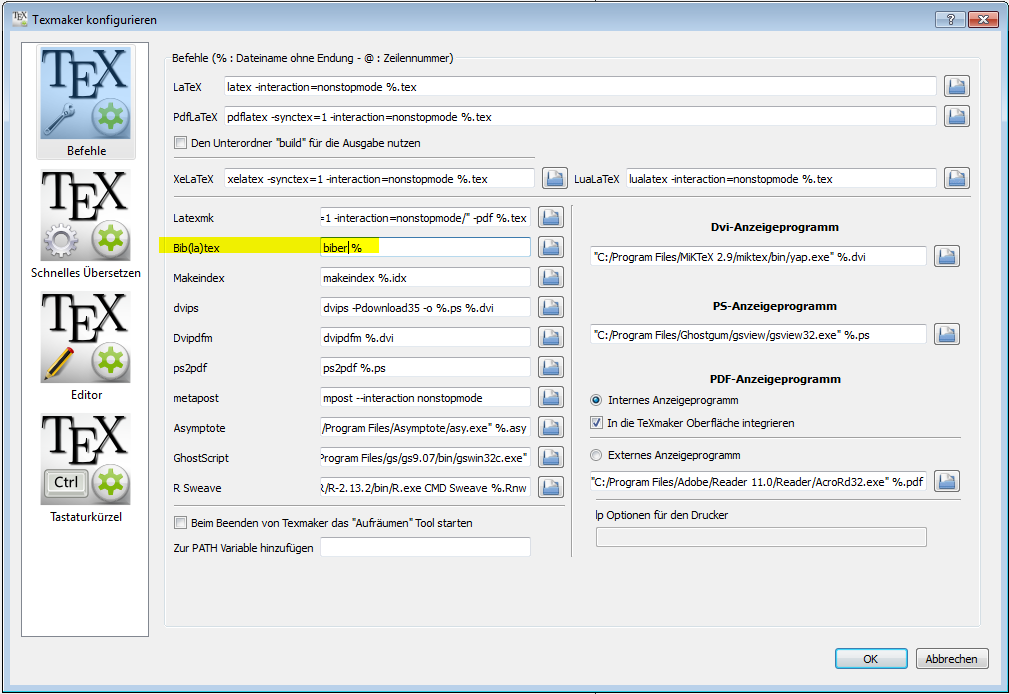
\includegraphics[width=0.8\linewidth]{Bilder/biber/Texmaker-Konfiguration.png}
            \captionof{figure}{Texmarker konfigurieren Bib(la)tex auf biber \% ändern.}
            \label{fig:Texmarker_konfigurieren}
        \end{figure}

        Damit alle Änderungen beim Kompilieren in der erzeugten PDF korrekt dargestellt werden, muss im Reiter \glqq Schnelles übersetzen\grqq \ die 2. Option \glqq PdfLaTeX + Bib(la)tex + PdfLaTeX (2x) + PDF anzeigen \grqq, wie in Abbildung \ref{fig:Texmarker_schnelles_uebersetzen} dargestellt, gewählt werden.
        
		\begin{figure}[H]
            \centering
            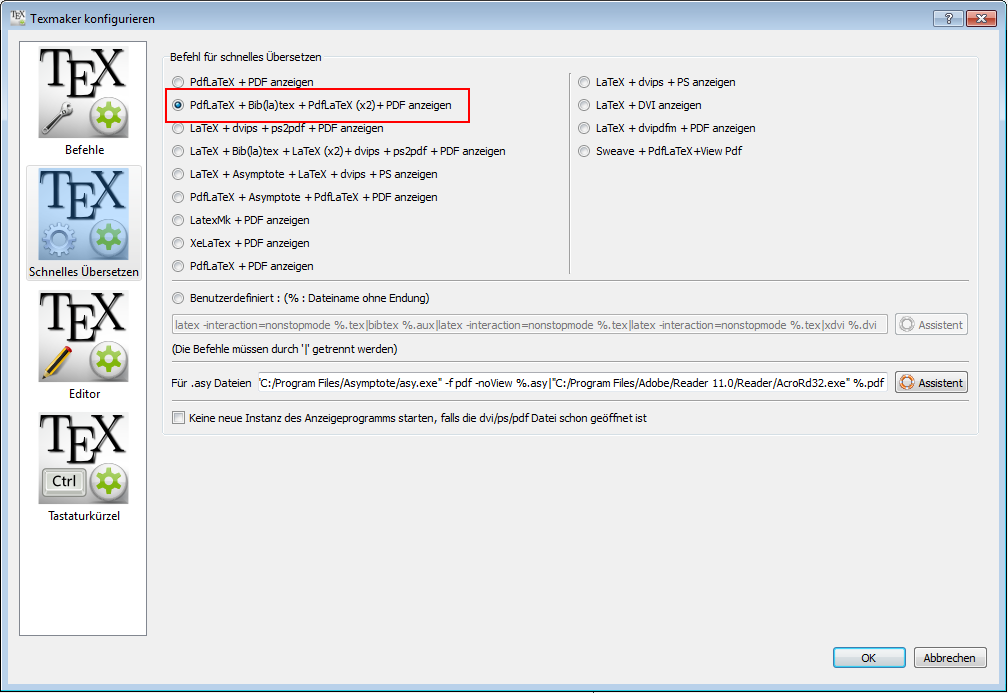
\includegraphics[width=0.8\linewidth]{Bilder/biber/Texmaker-schnelles_uebersetzen.png}
            \captionof{figure}{Texmarker konfigurieren schnelles Übersetzen.}
            \label{fig:Texmarker_schnelles_uebersetzen}
        \end{figure}

        Die ausführliche Variante ist notwendig, da beim ersten Ausführen des Befehls \glqq PdfLaTeX\grqq \ die \textbackslash cite Befehle aufgelöst werden. Durch den Befehl \glqq Bib(la)tex\grqq werden alle zum ersten Mal benutzten Literaturquellen aus der .bib in die .bbl Datei eingetragen. Das nachfolgende zweimalige kompilieren mit \glqq PdfLaTeX (2x)\grqq ist erforderlich, da beim ersten komplieren die captions und label der Tabellen und Abbildung erstellt werden und beim zweiten kompilieren das Inhaltsverzeichnis und die Verweise aus dem Text aktualisiert werden.


    	\pagebreak
		\section{Bitte unbedingt beachten!!!}
        \begin{enumerate}
            \item Bei Gleitkommazahlen ist die Punktschreibweise zu verwenden. (Beispiel 0.55)
            \item Der Name unter dem das Dokument abgespeichert wird ist wie folgt zu bilden: zuerst ein Präfix aus dem aktuellen Datum in JJMMTT Form, daran anschließend der eigentliche Name.
            \item Die entsprechende Studienarbeit ist vollständig abzugeben, das heißt mit allen dazugehörigen Materialien sowie den bearbeitbaren Dateien im zip-Format. Insbesondere eigens erstellte Abbildungen und Ähnliches sind in veränderbarer Form einzureichen. Ebenso die Studienarbeit ist neben einer pdf-Version auch in veränderbarer Form abzugeben.  Entsprechend den Anforderungen der jeweiligen Studienarbeit sind diese Dateien auf einem Datenträger zu übergeben. Immer gilt, die Dateien an Herrn Professor Herrmann per E-Mail zu senden.
            \item Es ist darauf zu achten, im Gesamtdokument einen einheitlichen Schriftsatz zu verwenden. Dies gilt auch für Abbildungen.
            \item Diagramme sind ausschließlich in hochauflösender Form und in schwarz/weiß zu erstellen. Dabei ist das Zeichnen mit Ti\textit{k}Z präferiert.
            \item Die Schriftzeichen in Tabellen, Abbildungen etc. müssen gleich groß (wie im Fließtext) sein.
            \item Die in Kapitel \ref{ch:struktur} vorgegebene Struktur ist einzuhalten.               
        \end{enumerate}

		\pagebreak

		%------------------------------------------------------------------------------
		%	Fließtext
		%------------------------------------------------------------------------------
		\section{Flie{\ss}text}
		\label{ch:fliesstext}
		Dieses Kapitel enthält Beispiele und Anleitungen für das Erstellen und Formatieren von Fließtext.

		%Beschreibung wie in LaTeX gegliedert wird
		\subsection{Gliederung}
		\label{ch:Gliederung}
		Die Gliederung in \LaTeX \ erfolgt über das Setzen von Sektionen und Paragraphen. Die ersten drei Gliederungsebenen werden mit den Befehlen \textit{\textbackslash section, \textbackslash subsection} und \textit{\textbackslash subsubsection} gebildet und werden auch in die Gliederung übernommen. Zwei zusätzliche Ebenen können mit \textit{\textbackslash paragraph} und \textit{\textbackslash subparagraph} gebildet werden. \LaTeX \ organisiert die Formatierung und Nummerierung automatisch.

		Vor jeder neuen \textit{section} muss mit \textit{pagebreak} ein Seitenumbruch erzeugt werden. So werden die einzelnen Kapitel getrennt.

		%Beschreibung der zu verwendenden Schriftgrößen
		\subsection{Schrift}
		\label{ch:schrift}
		In \LaTeX \ gibt es keine eigenen Schriftarten oder Schriftgrößen wie sie aus Word bekannt sind. Es existiert lediglich die hier verwendete Schriftart, die mit Hilfe von Befehlen formatiert werden kann. Im Umfeld der Fallstudiendokumentation sind nachfolgende Schriftgrößen mit ihren ungefähren Entsprechungen in MS Word dargestellt.

		\begin{table}[H]
			\centering
			\begin{tabular}{|l|l|l|l|}
				\hline  \textbackslash Large& \textbackslash large & \textbackslash normalsize & \textbackslash small \\
				\hline  17pt & 14pt & 13pt & 11pt   \\
				\hline
			\end{tabular}
			\caption{Schriftgrößen.} %Hinzufügen einer Tabellenbeschriftung
			\label{tab:schriftgroessen}
		\end{table}

		\subsection{Absätze}
		\label{ch:absaetze}
		Absätze werden über eine Leerzeile im Text gebildet. Normale Umbrüche können mit \textit{\textbackslash\textbackslash} erzeugt werden, allerdings wird dabei kein Abstand gebildet. Für diese Funktionalität muss das Paket \textit{parskip} eingebunden werden. Es folgt ein Beispiel:

		Lorem ipsum dolor sit amet, consetetur sadipscing elitr, sed diam nonumy eirmod tempor invidunt ut labore et dolore magna aliquyam erat, sed diam voluptua.

		%Neuer Absatz da eine Leerzeile vorranging
		Neue Absatz. At vero eos et accusam et justo duo dolores et ea rebum. Stet clita kasd gubergren, no sea takimata sanctus est Lorem ipsum dolor sit amet. \\ %Neue Teile da hier mit \\ umgebrochen wird
		Neuer Zeile. Lorem ipsum dolor sit amet, consetetur sadipscing elitr, sed diam nonumy eirmod tempor invidunt ut labore et dolore magna aliquyam erat, sed diam voluptua.

		\subsection{Hervorhebung}
		\label{ch:hervorhebung}
		Um Wörter ein einem Text hervorzuheben wird der befehlt \textit{\textbackslash emph} verwendet.
		\\ z.B.: Hier wird ein \emph{Wort} hervorgehoben.

		Um Befehle oder einzelne Syntaxelemente wie Methodennamen in einen Fliesstext einzubinden wird der Befehlt \textit{\textbackslash textit} verwendet.
		\\z.B.: Jede nichtabstarakte Klasse besitzt eine Methode \textit{constructor()}.

		\subsection{Sonderzeichen}
		\label{ch:zeichen}

		In \LaTeX \ sind viele Sonderzeichen bereits vorbelegt und müssen daher über eigene Befehle ausgegeben werden. Ergänzt wird die Liste durch eine Vielzahl an mathematischer Sonderzeichen. Die wichtigsten Sonderzeichen können unter \url{http://de.wikibooks.org/wiki/LaTeX-Kompendium:_Sonderzeichen} eingesehen werden.

		% Hier wird beschrieben, wie Modularisierung in \LaTeX realisiert werden kann.
		
% !TEX root = ../Vorlage.tex

\subsection{Modularisierung}
\LaTeX \ bietet die Möglichkeit der Modularisierung. Das heißt, dass Kapitel als Includes zu einem gesamten Dokument zusammengeführt werden können. Dabei werden alle Einstellungen in einem Hauptdokument vorgenommen und die Inhalte des Dokuments über den Befehl $\backslash include$ eingebunden. Die Includes definieren nur Dokumenteninhalt und verweisen auf ihr Hauptdokument. Als Beispiel wird dieser Punkt als Include eingebunden. Es muss dabei beachtet werden, dass nach jedem Include ein Seitenumbruch erfolgt. Daher wird die Verwendung von Includes nur für Sections empfohlen.



		\pagebreak
		%------------------------------------------------------------------------------
		%	Objekte
		%------------------------------------------------------------------------------
		\section{Objekte}
		\label{ch:objekte}
		Dieses Kapitel enthält Beispiele zum Einfügen von Abbildungen, Tabellen, etc..

		\subsection{Auflistung}

		Für Auflistungen wird die \textit{FHitemize}-Umgebung genutzt, wodurch der Zeilenabstand zwischen den Punkten verringert wird. Beispielcode kann dem Quelltext zu diesem Punkt entnommen werden.

		% Einfache Aufzählung
		\begin{FHitemize}
			\item Nur
			\item ein
			\item Beispiel
			% Unterpunkte
			\begin{FHitemize}
				\item mit
				\item Einrückung
			\end{FHitemize}
		\end{FHitemize}

		In Fallstudien im Umfeld des \gls{LIP} kommt es vor, dass eine Reihe an Parametern und Formeln zu Heuristiken, oder Verfahren dargestellt werden müssen. Bei einer Darstellung dieser Inhalte wird empfohlen, Tabulatoren zu verwenden, wie sie in Kapitel \ref{ch:parameter} dargestellt werden.

		\subsection{Referenzen}
		\label{ch:referenz}
		Um auf ein Bild, eine Tabelle, ein Kapitel, oder anderen Inhalten eine \LaTeX-Dokuments verweisen zu können, ist es notwendig das gewünschte Objekt mit einem Label zu versehen. Dies geschieht durch den Befehlt \textit{\textbackslash label} nach dem Objekt. Um die Referenzen besser verwenden zu können sind diese, entsprechend ihres Ziels, mit einem Präfix zu versehen. Daraus ergibt sich der Aufbau \textit{\textbackslash label\{\textless prefix\textgreater:\textless name\textgreater\}}. Dabei ist zu beachten, dass in der Labelbezeichnung außer des Präfixes keine Sonderzeichen oder Umlaute verwendet werden dürfen.

		% Liste mit Präfixen für Labelbeschriftung
		\begin{FHitemize}
			\item Bild fig:
			\item Tabelle tab:
			\item Kapitel ch:
			\item Code-Listing lst:
			\item Anhang app:
			\item Zitat eq:
		\end{FHitemize}

		% Wie kann ich auf ein Label refernezieren?
		Für die Referenzierung auf ein Label im Text wird der Befehl \textit{\textbackslash ref} durchgeführt.\\
		z.B. Verweis auf Kapitel der Referenzen in Kapitel \ref{ch:referenz}

		% Wie kann ich auf die Seite eines Labels refenzieren?
		Um auf die Seite eines Objekts zu referenzieren wird der Befehl \textit{\textbackslash refpage} verwendet.\\
		z.B. Dieses Kapitel befindet sich auf Seite \pageref{ch:referenz}

		%Beschreibung wie Fußnoten eingefügt werden
		\subsection{Fußnoten}
		\label{ch:fussnoten}
		Anmerkungen und Fußnoten sollen vermieden werden. Wenn die Nutzung unumgänglich ist (z.B. Hinweise auf Fehler in der Originalquelle), werden die Anmerkungen mit hochgestellten Ziffern durchnummeriert. Fußnoten werden über den Befehl \textit{\textbackslash footmark} in den Text eingebunden und mit \textit{\textbackslash footnotetext} die entsprechende Quelle geschaffen.

		% Hier wird der Verweis gesetzt
		z.B. eine Fußnote zu obigem Bild\footnotemark .
		% Das hier steht in der Fußzeile
		\footnotetext{Quelle: \url{http://www.osgi.org/Technology/WhatIsOSGi}}

		\subsection{Diagramme und Grafiken}
		\label{ch:bilder}
		Grafiken, Fotos oder Diagramme sollten drucktauglich sein und in der wiederzugebenden Größe in der Ausarbeitung an der gewünschten Position eingefügt werden. Dabei ist dieselbe Schriftart wie im Fließtext (Times New Roman) zu verwenden. Bei der Beschriftung ist darauf zu achten, dass diese mit einem Punkt beendet werden.\\
		Auf eine hochauflösende Darstellung ist zu achten. Bei Diagrammen ist dies gegeben, wenn bei einer Vergrößerung des Dokuments keine unscharfe Ansicht erfolgt. Die Grafiken sollen entweder in Visio erstellt und als PDFs eingebunden werden oder direkt in \LaTeX \ , durch Ti\textit{k}Z (siehe \ref{ch:TikZ}), erstellt werden. Hierbei ist Ti\textit{k}Z präferiert.
		
		\subsubsection{Microsoft Visio}		
		\label{ch:microsoft_visio}
		Microsoft Visio kann auf Rechnern der OTH Regensburg genutzt werden. Sollte eine Nutzung der OTH-Rechner vor Ort nicht möglich sein, kann eine Remotenutzung der CIP-Pool-Rechner erfolgen. Eine Anleitung ist im Anhang dieses Dokuments zu finden, siehe Anhang  \ref{app:remotenutzung}.\\

		Die Visio-Datein müssen für ihre Verwendung in \LaTeX \ um ihren Rand bereinigt werden. Dazu müssen unter Datei$\rightarrow$Optionen$\rightarrow$Menüband anpassen die Entwicklertools aktiviert werden. Anschließend müssen im Reiter Entwicklertools unter Menüpunkt Shapesheet anzeigen$\rightarrow$Zeichenblatt die Seitenränder der Druckeinstellungen auf 0mm gesetzt werden (vgl. Abbildung \ref{fig:visio}).

		\begin{figure}[H]
			\centering
			\includegraphics[width=0.8\linewidth]{Bilder/Visio.png}
			\captionof{figure}{Seitenränder in Visio auf 0 setzen.}
			\label{fig:visio}
		\end{figure}

		Beim Einbinden der Grafiken ist darauf zu achten, dass Beschriftungen klar zu lesen sind. Um dies sicherzustellen ist das Zeichenblatt in Visio auf eine Breite von 160 mm, was der Zeilenbreite der Vorlage entspricht, zu begrenzen. Die erstellten Zeichnungen müssen auf dieser Breite untergebracht werden. Ist die Grafik so umfangreich, dass diese Restriktion nicht eingehalten werden kann muss die Grafik an einer passenden Stelle geteilt werden.  Die Größeneinstellung des Zeichenblattes kann im Reiter Entwurf$\rightarrow$Format$\rightarrow$ Weitere Zeichenblattformate wie in Abbildung \ref{fig:Zeichenblatt} vorgenommen werden.

		\begin{figure}[H]
			\centering
			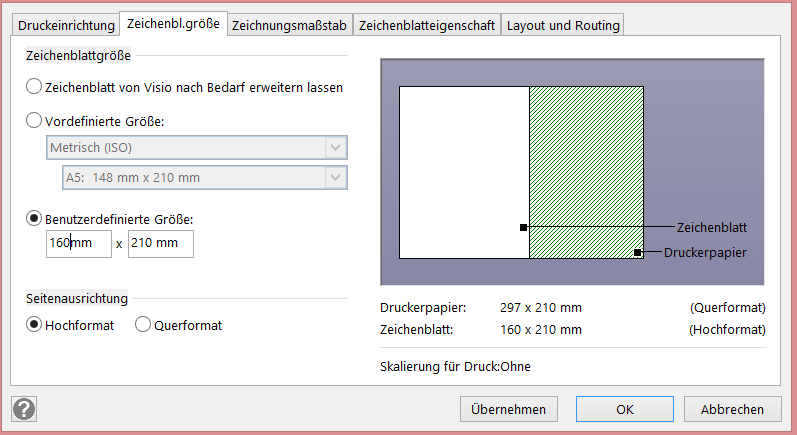
\includegraphics[width=1.0\linewidth]{Bilder/Zeichenblatt}
			\captionof{figure}{Zeichenbreite für Visio-Zeichnungen setzten.}
			\label{fig:Zeichenblatt}
		\end{figure}

		Für das Erstellen der gängigen Grafiktypen Gozintograph, Netzplan und Gantt-Diagramm liegen stehen im Laborverzeichnis unter Gemeinsames$\rightarrow$Dokumentvorlagen$\rightarrow$Office-Vorlagen entsprechende Schablonen für Visio zur Verfügung. Sollte der Umfang der Schablonen nicht ausreichen, können diese nach den jeweiligen Anforderungen erweitert werden. Es ist dabei darauf zu achten, dass eigene Grafiken keine Farben, sondern Grautöne und Muster als Kennzeichnungen beinhalten sollen.


        Vor der Erstellung eines PDFs sollte unbedingt der überflüssige Weißraum entfernt werden. Dies kann wie folgt erfolgen:

        \begin{FHitemize}
            \item Entwurf$\rightarrow$Format$\rightarrow$Größe an Zeichnung anpassen
        \end{FHitemize}

        Um aus einer Visio-Datei eine zu erstellen gibt es zwei Möglichkeiten.

        \begin{enumerate}
            \item Exportieren als PDF \\
            Unter \glqq Datei$\rightarrow$Exportieren$\rightarrow$PDF/XPS-Dokument erstellen\grqq \ \glqq PDF/XPS-Dokument erstellen\grqq \  auswählen.
            \item Speichern als PDF \\
            Unter \glqq Datei$\rightarrow$Speichern unter\grqq \ den Dateityp auf \glqq *.pdf\grqq ändern und anschließend speichern.
        \end{enumerate}

        Diese PDF-Datei kann wie ein Bild in \LaTeX \ eingebunden werden.

Ein Beispiel kann dem \LaTeX-Quelltext entnommen werden. Es ist zu beachten, dass alle verwendeten Bilder im Ordner \emph{Bilder} des Dokumentenverzeichnisses abgelegt werden und mit diesem Pfad eingebunden werden müssen.

		%Einbinden eines Bildes aus dem Ordner Bilder in der Dokumentenorderstruktur. Das Bild wir auf 80 % der gesamten Zeilenbreite skaliert. Mit captionof{} wird dem Bild eine Abbildungsbeschriftung hinzugefügt. Mit \centering wird das Bild zentriert. Mit \label{key} kann auf das Bild referenziert werden.
		\begin{figure}[H]
			\centering
			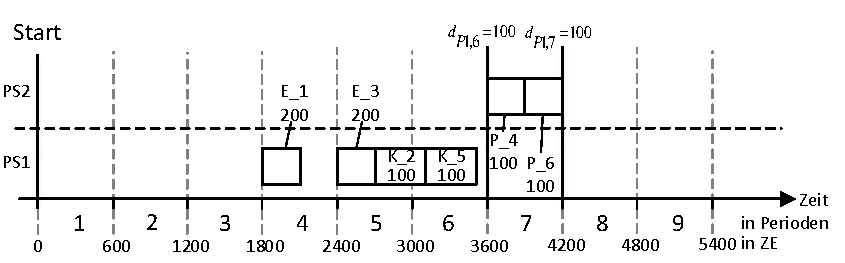
\includegraphics[width=1.0\linewidth]{Bilder/Netzplan_MRP2}
			\captionof{figure}{Beispiel Grafik Gantt-Diagramm.}
			\label{fig:osgi}
		\end{figure}

		Beim Einbinden der Grafiken kann über die Skalierung die Größe der Grafiken geregelt werden. Es ist darauf zu achten, dass die Grafiken möglichst einheitlich in ihrer Erscheinung sind. Das heißt, kleine Grafiken werden kleiner dargestellt und größere Grafiken werden auf die gesamte Textbreite skaliert. Die Bilder sollen also verhältnismäßig aufeinander abgestimmt sein. Sollten Grafiken angepasst werden, die bereits vorher für eine größere Zeichenblattbreite erstellt wurden, empfiehlt es sich die Breite auf 160 mm zu reduzieren und anschließen die Grafik für diese Größe zu skalieren. Anschließend wird die Schriftgröße reduziert bis sie die Grafik lesbar ist. Abschließend wird die Größe der Schriftart optimiert. Sollte der Platz für Beschriftungen nicht ausreichen kann nach belieben der Zeilenabstand der Beschriftungen unter Start$\rightarrow$Absatz$\rightarrow$Zeilenabstand reduziert werden.

        Die Datei \glqq Diagramme\_LaTex\_Beispiele\grqq \ enthält die folgenden mit Visio erstellten Diagramme und ist im Ordner Bilder der Latex-Vorlage zu finden.

        \textbf{Gantt Diagramm 1}

        \begin{figure}[H]
        \centering
        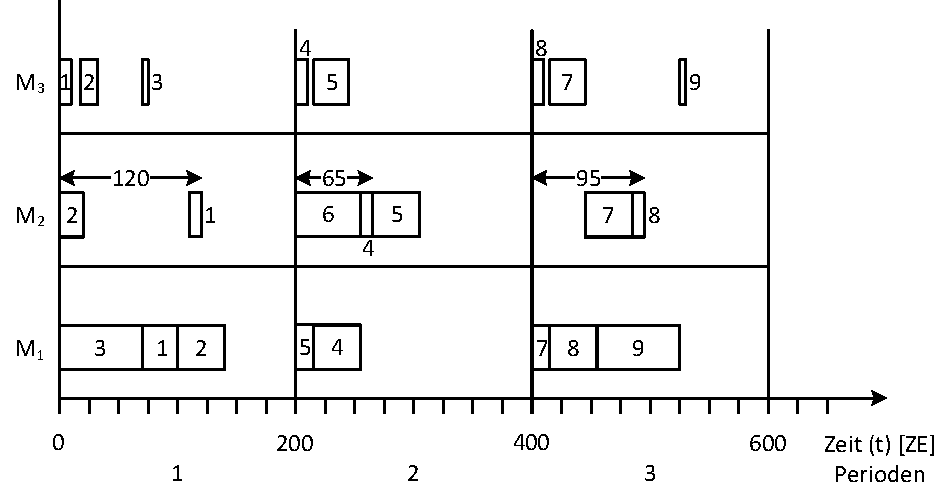
\includegraphics{Bilder/Gantt-Diagramm-1}
        \caption{Beschriftung des Gantt Diagramms}
        \label{fig:Gantt-Diagramm-1}
        \end{figure}

		
		\subsubsection{Grafiken mit \LaTeX \ erstellen: Ti\textit{k}Z}
		\label{ch:TikZ}
		Ti\textit{k}Z steht für "Ti\textit{k}Z ist \textit{kein} Zeichenprogramm". Das heißt, dass die Grafiken mittels Code erstellt werden.
		Zahlreiche Tutorials und Anleitungen sind im Internet frei zugänglich. Das sehr umfangreiche Benutzerhandbuch "Ti\textit{k}Z \& PGF Manual" \ wird empfohlen. Die Version vom 27.12.2020 des Handbuchs ist im Ordner dieser Vorlage hinterlegt.	Die zur Nutzung von Ti\textit{k}Z notwendigen Pakete sind in dieser Dokumentenvorlage integriert.\\
		
		Im Folgenden werden Beispiele aufgezeigt. Der Ti\textit{k}Z-Code kann dem Quelltext dieser Vorlage entnommen werden.\\
		
		Zur graphischen Lösung eines linearen Optimierungsproblems wurde die Abbildung in Ti\textit{k}Z erstellt.
		
	Gegeben sind die folgenden linearen Restriktionen. \\
		Variablen:
		\begin{tabularx}{\linewidth}{@{}p{2 cm}X}  %wichtig \keepXColumns muss gesetzt sein 
            $x_1 \in \mathbb{R} $&  \\
            $x_2 \in \mathbb{R} $ &  \\
		\end{tabularx}


		\begin{tabularx}{\linewidth}{@{}p{5 cm}X}  %wichtig \keepXColumns muss gesetzt sein
			$-x_1 + 2 \cdot x_2  \ge 4 $ 				& (1) \\
			$-4.5 \cdot x_1 + 3 \cdot x_2 \ge -1.5 $   	& (2) \\
			$x_1 \ge 0$   								& (3) \\
			$x_2 \ge 0$ 								& (4) \\ 
		\end{tabularx}


	und die folgende lineare Funktion: \\
		F($x_1$,$x_2$) = $1.5 \cdot x_1 + 0.5 \cdot x_2$  \\

	Lösen Sie die folgenden linearen Optimierungsprobleme:

		\begin{enumerate} [leftmargin=*, label= (\alph*)]
			\item Maximiere F($x_1$,$x_2$) unter den Restriktionen (d.h. s.t.) (1) bis (4).            
            \item Maximiere F($x_1$,$x_2$) s.t. (1) bis (4)  sowie $x_2 \le 3.25$ (5).\\       
		\end{enumerate}	
		
	
	
	Nachfolgende Abbildung zeigt die Lösung für Teilaufgabe b).
	Der gesamte dazugehörige Ti\textit{k}Z-Code ist im TeX-Dokument dieser Vorlage zu finden. Generell wurden für das Erstellen der Abbildung \ref{fig:TikZ-LinOpt} folgende Schritte durchgeführt:
	\begin{enumerate}
            \item Erstellen und Formatieren des Koordinatensystems,
            \item Einzeichnen des Lösungsraums,
            \item Einzeichnen der Restriktionen,
            \item Einzeichnen der Zielfunktion,
            \item Einzeichnen des Optimums.\\
    \end{enumerate}
	
	
			
		
		\begin{figure}[H]
		\centering
			
				\begin{tikzpicture}[scale=1] %wenn scale=2, dann ergänze: font=\tiny

		
		\node[yshift=-0.18cm] at (0:0){0};	% Beschriftung Nullpunkt	
		
		\begin{axis}[
		width=12cm, height=12cm, %Größe der Abbildung
		axis lines=middle,
		axis equal,
		axis line style={-latex}, %Pfeil bei Achse nur in eine Richtung, ansonsten {latex-latex}
		%x-Achse:%		
			domain=-18:30, %x-Achsen-Bereich, in dem Plots dargestellt werden können
			smooth,
			xmin=-0.1,xmax=5.9, %Bereich der x-Achse
			tick style={line width=.5pt,black},	tick label style={fill=white},
			xtick={0, 1, 2, ..., 5}, 
			xlabel=$x_1$, xlabel style={fill=white,right,inner xsep=2pt}, %x-Achsenbeschriftung   	
      	%y-Achse:%
      		restrict y to domain=-18:30, %y-Achsen-Bereich, in dem Plots dargestellt werden können
      		ymin=-0.1,ymax=5.9, %Bereich der y-Achse
      		ytick={0,1, 2, ..., 5}, ylabel=$x_2$, ylabel style={fill=white,above,inner ysep=2pt},  %y-Achsenbeschriftung  
      	%minor tick num=4, minor tick length=4pt, minor tick style={line width=.5pt}, %Teilstriche x- und y-Achse
      	samples=100, %Punkte je Plot
		set layers=axis on top   ,
		axis background/.style={fill=white} 	
    	]
		
		%Lösungsraum:%
		\addplot[pattern=north east lines,pattern color=black!50] (0,2) -- (2.5,3.25) -- (0,3.25)\closedcycle; %Lösungsraum
		
		
		%Gleichung 1:%		
		\addplot[black] {0.5*x + 2}; %Gleichung 2: -x1 + 2x2 >= 4
			\node at (4.5,4){(1)};
			%Koordinaten für Richtungspfeil "oben-rechts" für Gleichung 1:
				\coordinate (a) at (5,4.5);
				\coordinate (b) at ($ (5,4.5)!0.45cm!90:(5.5,4.75) $);  %% 
			%Koordinaten für Richtungspfeil "unten-links" für Gleichung 1:	%Siehe TikZ-Anleitung S. 151 f.
				\coordinate (c) at (0.7,2.35);
				\coordinate (d) at ($ (0.7,2.35)!0.45cm!90:(1,2.5) $);  %% Startkoordinate -- Länge der Orthogonale -- 90 Grad = Orthogonale bestimmen (alternativ 180 Grad)-- Endkoordinate %%
			%Richtungspfeile für Gleichung 1:	
			\draw[>=Straight Barb,->] (a) -- (b);
			\draw[>=Straight Barb,->] (c) -- (d);		
		
		%Gleichung 2:%
		\addplot[black] {1.5*x - 0.5}; %Gleichung 3: -4.5x1 + 3x2 >= -1.5
			\node at (4,5.15){(2)};
			%Koordinaten für Richtungspfeil "oben-rechts" für Gleichung 2:
				\coordinate (e) at (3.5,4.75);
				\coordinate (f) at ($ (3.5,4.75)!0.45cm!90:(4,5.5) $);  %% 
			%Koordinaten für Richtungspfeil "unten-links" für Gleichung 2:
				\coordinate (g) at (1.5,1.75);
				\coordinate (h) at ($ (1.5,1.75)!0.45cm!90:(2,2.5) $);
			%Richtungspfeile für Gleichung 2:	
			\draw[>=Straight Barb,->] (e) -- (f);
			\draw[>=Straight Barb,->] (g) -- (h);		
		
			%Gleichung 3:%		
		\draw [black] (0,0) -- (0,6); %Gleichung 3: x1 >= 0;	
			\node at (0.2,5.4){(3)};
			\coordinate (i) at (0,5.2);
			\coordinate (j) at ($ (i)!0.45cm!90:(0,0.5) $);
			\coordinate (k) at (0,0.5);
			\coordinate (l) at ($ (k)!0.45cm!-90:(0,5.2) $);
			\draw[>=Straight Barb,->] (i) -- (j);
			\draw[>=Straight Barb,->] (k) -- (l);	
				
		
		%Gleichung 4:%			
		\draw [black] (0,0) -- (6,0); %Gleichung 4: x2 >= 0
			\node at (4.9,0.2){(4)};
			%m,n,o,p
			\coordinate (m) at (2.5,0);
			\coordinate (n) at ($ (m)!0.45cm!90:(5.2,0) $);
			\coordinate (o) at (5.2,0);
			\coordinate (p) at ($ (o)!0.45cm!-90:(2.5,0) $);
			\draw[>=Straight Barb,->] (m) -- (n);
			\draw[>=Straight Barb,->] (o) -- (p);
	
		%Gleichung 5:%		
		\addplot[black] {3.25}; %Gleichung 5: x2 <= 3.25
			\node at (4.8,3.05){(5)};
			%q,r,s,t
			\coordinate (q) at (1,3.25);
			\coordinate (r) at ($ (q)!0.45cm!-90:(5.2,3.25) $);
			\coordinate (s) at (5.2,3.25);
			\coordinate (t) at ($ (s)!0.45cm!90:(1,3.25) $);
			\draw[>=Straight Barb,->] (q) -- (r);
			\draw[>=Straight Barb,->] (s) -- (t);

		
		
		%Zielfunktion:%
		\addplot[black, dashed] {-3*(x-1)} ; %Zielfunktion: Maximiere 1.5x1 + 0.5x2  %x-shift in Höhe von 1 zur Darstellung in Koordinatensystem%
			\node at (0.78,1.5) {(ZF)}; %Beschriftung Zielfunktion
			%Koordinaten für Richtungspfeil:
				\coordinate (u) at (0.1,2.7); %Pfeil beginnt bei x=0.3 und y=(-3*(0.3-0.88))=1.74
				\coordinate (v) at ($ (0.1,2.7)!0.45cm!90:(0.5,1.5) $);  %Pfeil als Orthogonale zwischen Punkt i und Punkt j (x=0.5; y=(-3*(0.5-0.88))=1.14)
			
			%Koordinaten für Richtungspfeil:
				\coordinate (w) at (0.6,1.2);
				\coordinate (x) at ($ (0.6,1.2)!0.45cm!90:(0.7,0.9) $);  %% 
				
			%Richtungspfeile:	
				\draw[>=Straight Barb,->] (u) -- (v);	
				\draw[>=Straight Barb,->] (w) -- (x);
				
			\draw[black](2.5,3.25)circle[radius=3pt] node [align=center, below right]{OP};%Optimaler Punkt
		
		\end{axis}
		
		%%Legende
		\node at (-0.1,-1.2)[label=right: OP: Optimaler Punkt;\quad    ZF: Zielfunktion;]{};
		\node[draw, minimum width=0.7cm,minimum height=0.3cm,pattern=north east lines,pattern color=black!50](Legend) at (8.5,-1.2)[label=right: Lösungsraum]{}; 		
		
		\end{tikzpicture}
		\caption{eine mit Ti\textit{k}Z erstellte grafische Darstellung des Linearen Optimierungsproblems (Aufgabe b)).}
		\label{fig:TikZ-LinOpt}
		\end{figure}	
	
	Graphen werden in dieser Vorlage zumeist mit dem Befehl \textbackslash addplot dargestellt. Dazu sind die Gleichungen in der Form $a\cdot x + b $ zu hinterlegen. Entsprechend gilt es, vorher die Gleichungen in die Normalform \quad $y = a \cdot x + b$ \quad bzw. \quad $y \leq a \cdot x + b$ \quad oder \quad $y \geq a \cdot x + b$ \quad zu bringen. Der Einfachheit halber werden Graphen, die parallel zur x- oder y-Achse verlaufen, in dieser Vorlage nicht durch \textbackslash addplot eingefügt, sondern durch Angabe von Start- und Zielkoordinate als Linie gezeichnet. Beispielsweise wird Restriktion (5) auf diese Weise gezeichnet (\textbackslash draw [black] (0,3.25) -- (6,3.25);).
	
	Bei den Beschriftungen der Graphen werden sogenannte "nodes" \ verwendet. Diese können durch genaue Angabe von Koordinaten angeordnet werden. Für die Beschriftung des optimalen Punkts wird beispielsweise folgendes hinterlegt:  \textbackslash node at (2.7, 3.1)\{OP\}.\\ \\
	Die Beschriftungspfeile der einzelnen Graphen werden jeweils als Orthogonale zur Strecke zwischen zwei Punkten auf dem entsprechenden Graph hinterlegt. Für jeden dieser Richtungspfeile sind somit zwei Punkte auf dem Graphen als Koordinaten zu definieren, zwischen denen eine Strecke angenommen wird, zu der das Lot gefällt wird. Dafür wird zunächst der Punkt gewählt, bei dem der Richtungspfeil beginnen soll, und durch \textbackslash coordinate definiert. Ein weiterer Punkt auf dem Graphen ist anzugeben, damit zur Strecke zwischen diesem und der ersten Koordinate das Lot gefällt werden kann. Durch Angabe der gewünschten Länge des Pfeils wird dann die Zielkoordinate bestimmt. Der Richtungspfeil wird im Anschluss zwischen der Start- und Zielkoordinate gezeichnet.
	
	Folgender Code wird für den linken Richtungspfeil von Gleichung (2) hinterlegt. \\
	
	\begin{lstlisting}			
			\coordinate (g) at (1.5,1.75);
			\coordinate (h) at ($ (g)!0.45cm!90:(3.5,4.75) $);
			\draw[>=Straight Barb,->] (g) -- (h);
	\end{lstlisting}	
	\captionof{lstlisting}{Ti\textit{k}Z-Code für den linken Richtungspfeil von Gleichung (2).}
	\label{lst:TikZ-Richtungspfeil}
	\vspace{0.5cm}
	Koordinate (g) stellt die Startkoordinate dar, Koordinate (h) die Zielkoordinate für den Richtungspfeil. Bei einem x-Wert von 1.5 ergibt das Einsetzen in die Normalform von Gleichung (2) ($x_2 = 1.5 \cdot x - 0.5 = 1.5 \cdot 1.5 - 0.5$)  die y-Koordinate mit dem Wert 1.75. Somit ist die Startkoordinate (1.5,1.75) - dort beginnt der Richtungspfeil. Um den Richtungspfeil genau in 90 Grad zum Graphen auszurichten, wird die Orthogonale verwendet. Dazu ist ein zweiter Punkt auf dem Graphen zu wählen (der Einfachheit halber wird als zweite Koordinate der Punkt gewählt, der zugleich als Startkoordinate für den zweiten Richtungspfeil von Gleichung (2) verwendet wird). Diese Koordinate wird wiederum durch das Festlegen des x-Werts und dem Einsetzen in die Normalform von Gleichung (2) bestimmt. Man erhält die Koordinate (3.5, 4.75). Die Koordinate, die 0.45cm entfernt von Startkoordinate g und im rechten Winkel zur Strecke zwischen g und der Koordinate (3.5,4.75) ist, ist die Zielkoordinate - dort endet der Richtungspfeil. Abschließend wird der Richtungspfeil zwischen g und h gezeichnet. Für eine Ausrichtung des Richtungspfeils in die entgegengesetzte Richtung kann ein Winkel gleich -90 (Grad) verwendet werden.\\
	
	Folgende Darstellung zeigt diese Überlegungen nochmals in Detail.
	
		\begin{figure}[H]
		\centering
		\begin{tikzpicture}[scale=2]
			\draw[-] (1,1) -- (4,5.5) node [sloped,midway,above] {Gleichung (2)}; % Gleichung 2
			\coordinate (g) at (1.5,1.75);		
			\node at (1.7, 1.7){(g)};
			\fill[grey](3.5,4.75)circle[radius=1pt];
			\coordinate (z) at (3.5,4.75);
			\node at (4.0, 4.6){(3.5,4.75)};
			\coordinate (h) at ($ (g)!0.45cm!90:(3.5,4.75) $);
			\fill[grey](h)circle[radius=1pt];
			\node at (1, 2.15){(h)};
			\path[] (z) -- (g) -- (h) pic [fill opacity=1.0, "$\cdot$", draw, -] {angle=z--g--h};
			\coordinate (j) at ($ (g)!0.425cm!90:(3.5,4.75) $);
			\draw[>=Straight Barb,->] (g) -- (j); %line width=0.3mm, 
			\fill[grey](1.5,1.75)circle[radius=1pt];	
		\end{tikzpicture}
		\caption{detaillierte Darstellung des linken Richtungspfeils für Gleichung (2).}
		\label{fig:TikZ-Richtungspfeil}
		\end{figure}
	
	
	In obigem Beispiel (Abbildung \ref{fig:TikZ-LinOpt}) ist es weiterhin notwendig, die Zielfunktion entsprechend zu verschieben, damit diese im Koordinatensystem angezeigt wird. Dies wurde direkt in der Gleichung der Zielfunktion durch Subtraktion eines geeigneten Werts von x verwirklicht. Die ursprüngliche Zielfunktion in diesem Beispiel lautet in Normalform: $x_2 = -3 \cdot x_1$. Durch Subtraktion von 1 von $x_1$ wird der Graph der Zielfunktion geeignet nach rechts verschoben. Die dadurch resultierende Funktion $x_2 = -3 \cdot (x_1 - 1)$ ist im oberen rechten Quadranten des Koordinatensystems sichtbar.\\
	Abbildung \ref{fig:TikZ-ZF} stellt die horizontale Verschiebung der Zielfunktion graphisch dar. 
	
	\begin{figure}[H]
		\centering
		\begin{tikzpicture}[scale=1] %wenn scale=2, dann ergänze: font=\tiny
		%\node[yshift=-0.18cm] at (0:0){0};	% Beschriftung Nullpunkt	
		
		\begin{axis}[
		width=12cm, height=12cm, %Größe der Abbildung
		axis lines=middle,
		axis equal,
		axis line style={-latex}, %Pfeil bei Achse nur in eine Richtung, ansonsten {latex-latex}
		%x-Achse:%		
			domain=-18:30, %x-Achsen-Bereich, in dem Plots dargestellt werden können
			smooth,
			xmin=-4.5,xmax=4.9, %Bereich der x-Achse
			tick style={line width=.5pt,black},	
			%tick label style={fill=white},
			xtick={-4, -3,..., 4}, 
			xlabel=$x_1$, xlabel style={fill=white,right,inner xsep=2pt}, %x-Achsenbeschriftung   	
      	%y-Achse:%
      		restrict y to domain=-18:30, %y-Achsen-Bereich, in dem Plots dargestellt werden können
      		ymin=-4.5,ymax=4.9, %Bereich der y-Achse
      		ytick={-4,-3,-2,-1,0, 1, 2, 3,4}, ylabel=$x_2$, ylabel style={fill=white,above,inner ysep=2pt},  %y-Achsenbeschriftung  
      	%minor tick num=4, minor tick length=4pt, minor tick style={line width=.5pt}, %Teilstriche x- und y-Achse
      	samples=100, %Punkte je Plot
		set layers=axis on top   ,
		axis background/.style={fill=white} 	
    	]	
	
		
		%Zielfunktion:%
		\addplot[black] {-3*(x+1)};
		\draw (-2,3) -- (-1,0) node [sloped, at start, below]{$x_2 = -3 \cdot (x_1 +1)$};
		\addplot[black] {-3*(x)};
		\draw (1,-3) -- (2,-6) node [sloped, at start, above]{$x_2 = -3 \cdot x_1$};
		\addplot[black] {-3*(x-1)};
		\draw (2,-3) -- (3,-6) node [sloped, at start, above]{$x_2 = -3 \cdot (x_1 -1)$};
		\end{axis}		
		\end{tikzpicture}	
		\caption{horizontale Verschiebung eines Graphen durch Anpassung der Funktion.}
		\label{fig:TikZ-ZF}
		\end{figure}	
		
	
Zur Darstellung der Produktstruktur wurde ein Gozintograph mit Ti\textit{k}Z erstellt. 


Für das Erstellen des Gozintographen wurden folgende Schritte durchgeführt:
	\begin{enumerate}
            \item Darstellen der Produktstruktur von Endprodukt 1 (P1) lediglich mit konvergierender Struktur und ohne Verbindungen über mehrere Stufen hinweg (siehe Abbildung \ref{fig:TikZ-Gozintograph-Schritt1}),
            \item Hinzufügen von Endprodukt 2, ebenso ohne Verbindungen über mehrere Stufen hinweg (siehe Abbildung \ref{fig:TikZ-Gozintograph-Schritt2}),
            \item Hinzufügen der Verbindungslinien zwischen den einzelnen Produkten und Produktstufen (siehe Abbildung \ref{fig:TikZ-Gozintograph}).\\
    \end{enumerate}

\begin{figure}[H]
    \centering
		%\usepackage{tikz-qtree,tikz-qtree-compat} %Paket zu Beginn des Dokuments bereits hinterlegt
		\begin{tikzpicture}[scale=2, sibling distance=.25cm, font=\tiny, every node/.style={draw,rectangle,inner sep=4pt,minimum width=20pt, minimum height=12pt}, latex-]
			\Tree 	
					[.\node (P1) {P1}; %Endprodukt P1			
						\edge node[draw=none, very near end, above] {1}; %Beschriftung: "draw=none" zur Vermeidung von Umrahmung, "very near end" zur Anordnung nahe des Vorprodukts, "above" zur Ausrichtung über Pfeil (Alternativ: "below", "right", "left")%
        				[.\node (A1) {A1}; %Vorprodukt A1
        				]
        				\edge node[draw=none, very near end, above] {2}; %Beschriftung P1 bis B1
        				[.\node (B1) {B1}; %Vorprodukt B1						
							\edge node[draw=none, very near end, above] {2}; %Beschriftung B1 bis D1           		
           					[.\node (D1) {D1}; %Vorprodukt D1          			
           						\edge node[draw=none, very near end, above] {2}; %Beschriftung D1 bis F1  
           						[.\node (F1) {F1}; ] %Vorprodukt F1					
								\edge node[draw=none, very near end, above] {2}; %Beschriftung D1 bis G1             			
           						[.\node (G1) {G1}; ] %Vorprodukt G1
           					]           				
           					\edge node[draw=none, very near end, above] {2}; %Beschriftung B1 bis E1
           					[.\node (E1) {E1}; %Vorprodukt E1
           						\edge node[draw=none, right] {2}; %Beschriftung E1 bis H1
           						[.\node (H1) {H1};] %Vorprodukt H1
           					]
           				]
          			]   
    
		\end{tikzpicture}		
        			
		\caption{Schritt 1 für die Erstellung des gewünschten Gozintographen in Ti\textit{k}Z.}
		\label{fig:TikZ-Gozintograph-Schritt1}
	\end{figure}


	\begin{figure}[H]
    \centering
		%\usepackage{tikz-qtree,tikz-qtree-compat} %Paket zu Beginn des Dokuments bereits hinterlegt
		\begin{tikzpicture}[scale=2, sibling distance=.25cm, font=\tiny, every node/.style={draw,rectangle,inner sep=4pt,minimum width=20pt, minimum height=12pt}, latex-]
			\Tree 	
					[.\node (P1) {P1}; %Endprodukt P1			
						\edge node[draw=none, very near end, above] {1}; %Beschriftung: "draw=none" zur Vermeidung von Umrahmung, "very near end" zur Anordnung nahe des Vorprodukts, "above" zur Ausrichtung über Pfeil (Alternativ: "below", "right", "left")%
        				[.\node (A1) {A1}; %Vorprodukt A1
        				]
        				\edge node[draw=none, very near end, above] {2}; %Beschriftung P1 bis B1
        				[.\node (B1) {B1}; %Vorprodukt B1						
							\edge node[draw=none, very near end, above] {2}; %Beschriftung B1 bis D1           		
           					[.\node (D1) {D1}; %Vorprodukt D1          			
           						\edge node[draw=none, very near end, above] {2}; %Beschriftung D1 bis F1  
           						[.\node (F1) {F1}; ] %Vorprodukt F1					
								\edge node[draw=none, very near end, above] {2}; %Beschriftung D1 bis G1             			
           						[.\node (G1) {G1}; ] %Vorprodukt G1
           					]           				
           					\edge node[draw=none, very near end, above] {2}; %Beschriftung B1 bis E1
           					[.\node (E1) {E1}; %Vorprodukt E1
           						\edge node[draw=none, right] {2}; %Beschriftung E1 bis H1
           						[.\node (H1) {H1};] %Vorprodukt H1
           					]
           				]
          			]   
          			
    		\begin{scope}[xshift=3cm] %Zur Ausrichtung des weiteren Endprodukts (P2) neben erstem Endprodukt (P1)%
    
    		\Tree 
    				[. \node (P2){P2}; %Endprodukt P2  				
    					\edge node[draw=none, very near end, above right] {1}; %Beschriftung P2 bis C1
          				[.\node (C1) {C1}; %Vorprodukt C1         				
          	  				\edge [draw=none]; %Vermeidung der Verbindungslinie von Produkt C1 zu Vorprodukt Teil 1%
          					[.\node[draw=none] {};
          					\edge [draw=none]; %Vermeidung der Verbindungslinie von Produkt C1 zu Vorprodukt Teil 2%         			
          					[.\node (I1) {I1}; %Vorprodukt I1
          					]
          					]	
          				]
					]          			
    		\end{scope}

		\end{tikzpicture}		
        			
		\caption{Schritt 2 für die Erstellung des gewünschten Gozintographen in Ti\textit{k}Z.}
		\label{fig:TikZ-Gozintograph-Schritt2}
	\end{figure}

	Mit Schritt 3 erfolgt das Einzeichnen der noch gewünschten Verbindungslinien. Dazu werden entsprechende Pfeile von der Unterseite eines Kästchens ([].south) zur Oberseite eines darunterliegenden Kästchens ([].north) gezeichnet. Im Anschluss hat der Gozintograph die gewünschte Form (siehe Abbildung \ref{fig:TikZ-Gozintograph}).\\ 
	Auch hier wurden die Beschriftungen mittels "nodes" \ durchgeführt. Dazu sei auf die Erläuterungen zu Abbildung \ref{fig:TikZ-LinOpt} verwiesen. Durch Anpassung der einzelnen Schritte kann der Gozintograph den eigenen Anforderungen gemäß abgeändert werden.\\
\begin{figure}[H]
    \centering
		%\usepackage{tikz-qtree,tikz-qtree-compat} %Paket zu Beginn des Dokuments bereits hinterlegt
		\begin{tikzpicture}[scale=2, sibling distance=.25cm, font=\tiny, every node/.style={draw,rectangle,inner sep=4pt,minimum width=20pt, minimum height=12pt}, latex-]
			\Tree 	
					[.\node (P1) {P1}; %Endprodukt P1			
						\edge node[draw=none, very near end, above] {1}; %Beschriftung: "draw=none" zur Vermeidung von Umrahmung, "very near end" zur Anordnung nahe des Vorprodukts, "above" zur Ausrichtung über Pfeil (Alternativ: "below", "right", "left")%
        				[.\node (A1) {A1}; %Vorprodukt A1
        				]
        				\edge node[draw=none, very near end, above] {2}; %Beschriftung P1 bis B1
        				[.\node (B1) {B1}; %Vorprodukt B1						
							\edge node[draw=none, very near end, above] {2}; %Beschriftung B1 bis D1           		
           					[.\node (D1) {D1}; %Vorprodukt D1          			
           						\edge node[draw=none, very near end, above] {2}; %Beschriftung D1 bis F1  
           						[.\node (F1) {F1}; ] %Vorprodukt F1					
								\edge node[draw=none, very near end, above] {2}; %Beschriftung D1 bis G1             			
           						[.\node (G1) {G1}; ] %Vorprodukt G1
           					]           				
           					\edge node[draw=none, very near end, above] {2}; %Beschriftung B1 bis E1
           					[.\node (E1) {E1}; %Vorprodukt E1
           						\edge node[draw=none, right] {2}; %Beschriftung E1 bis H1
           						[.\node (H1) {H1};] %Vorprodukt H1
           					]
           				]
          			]   
          			
    		\begin{scope}[xshift=3cm] %Zur Ausrichtung des weiteren Endprodukts (P2) neben erstem Endprodukt (P1)%
    
    		\Tree 
    				[. \node (P2){P2}; %Endprodukt P2  				
    					\edge node[draw=none, very near end, above right] {1}; %Beschriftung P2 bis C1
          				[.\node (C1) {C1}; %Vorprodukt C1         				
          	  				\edge [draw=none]; %Vermeidung der Verbindungslinie von Produkt C1 zu Vorprodukt Teil 1%
          					[.\node[draw=none] {};
          					\edge [draw=none]; %Vermeidung der Verbindungslinie von Produkt C1 zu Vorprodukt Teil 2%         			
          					[.\node (I1) {I1}; %Vorprodukt I1
          					]
          					]	
          				]
					]          			
    		\end{scope}
        
    	%Beschriftungen der "untypischen" Verbindungen zwischen verschiedenen Abzweigungen  
			\draw [arrows = {Latex[width=7pt, length=7pt]-}, thick] (E1.south) -- node[draw=none,midway, below] {\normalsize{1}} (G1.north); % Verbindung und Beschriftung E1 bis G1
			\draw [arrows = {Latex[width=7pt, length=7pt]-}, thick] (A1.south) -- node[draw=none,midway, below left] {\normalsize{3}} (F1.north); % Verbindung und Beschriftung A1 bis F1
			\draw [arrows = {Latex[width=7pt, length=7pt]-}, thick] (C1.south) -- node[draw=none,midway, below] {\normalsize{3}} (E1.north); % Verbindung und Beschriftung C1 bis E1
			\draw [arrows = {Latex[width=7pt, length=7pt]-}, thick] (C1.south) -- node[draw=none, very near end, above right] {\normalsize{2}} (I1.north); % Verbindung und Beschriftung C1 bis I1
		\end{tikzpicture}		
        			
		\caption{ein mit Ti\textit{k}Z erstellter Gozintograph.}
		\label{fig:TikZ-Gozintograph}
	\end{figure}

Weitere Abbildungen von Gozintographen sind im Folgenden dargestellt:

Abbildung \ref{fig:TikZ-Gozintograph2} zeigt einen Gozintographen mit Kreisen und divergierender Erzeugnisstruktur, Abbildung \ref{fig:TikZ-Gozintograph3} zeigt einen Gozintographen mit Angabe der Dispositionsstufen.

\begin{figure}[H]
    \centering
		%\usepackage{tikz-qtree,tikz-qtree-compat} %Paket zu Beginn des Dokuments bereits hinterlegt
		\begin{tikzpicture}[scale=2, level distance=1.5cm, sibling distance=.25cm, font=\tiny, every node/.style={draw,circle,inner sep=4pt,minimum width=20pt, minimum height=12pt}, latex-]
			\Tree 	
					[.\node (P1) {P1}; %Endprodukt P1			
						\edge node[draw=none, very near end, above left] {1}; %Beschriftung P1 bis A1%
        				[.\node (A1) {A1}; %Vorprodukt A1
        				]
          			]           			
    		\begin{scope}[xshift=1.25cm] %Zur Ausrichtung des weiteren Endprodukts (P2) neben erstem Endprodukt (P1)%
    		\Tree 
    				[. \node (P2){P2}; %Endprodukt P2  				
    					\edge [draw=none] {}; %Vermeidung der Verbindungslinie von Produkt P2 zu C1
          				[.\node (C1) {C1}; %Vorprodukt C1         				
          	  				\edge node [draw=none, near end, above right] {1}; 
          					[.\node(E1) {E1};      			
          					]	
          				]
					]          			
    		\end{scope}
        
        	\begin{scope}[xshift=2.5cm] %Zur Ausrichtung des weiteren "Phantom"-Endprodukts rechts neben P2 (P1)%
    		\Tree 
    				[.\node[draw=none] {}; % Kein Endprodukt in dritter "Spalte"
    					\edge [draw=none] {}; %Vermeidung der Verbindungslinie von oberem Kreis zu mittlerem Kreis
          				[.\node (P4) {P4}; %Vorprodukt P4         					
          				]
					]          			
    		\end{scope}
    	
    	%Beschriftungen der "untypischen" Verbindungen zwischen verschiedenen Abzweigungen  
			\draw [arrows = {Latex[width=7pt, length=7pt]-}, thick] (P2.south) -- node[draw=none,midway, below] {\normalsize{1}} (A1.north); % Verbindung und Beschriftung P2 bis A1
			\draw [arrows = {Latex[width=7pt, length=7pt]-}, thick] (A1.south) -- node[draw=none,midway, below left] {\normalsize{3}} (E1.north); % Verbindung und Beschriftung A1 bis E1
			\draw [arrows = {Latex[width=7pt, length=7pt]-}, thick] (P4.south) -- node[draw=none,midway, below] {\normalsize{3}} (E1.north); % Verbindung und Beschriftung P4 bis E1
		\end{tikzpicture}		
        			
		\caption{ein weiterer, mit Ti\textit{k}Z erstellter Gozintograph.}
		\label{fig:TikZ-Gozintograph2}
	\end{figure}

\begin{figure}[H]
    \centering
		%\usepackage{tikz-qtree,tikz-qtree-compat} %Paket zu Beginn des Dokuments bereits hinterlegt
		\begin{tikzpicture}[scale=2, level distance=1.5cm, sibling distance=.25cm, font=\tiny, every node/.style={draw,circle,inner sep=4pt,minimum width=20pt, minimum height=12pt}, latex-]
			\Tree 	
					[.\node (P1) {P1}; %Endprodukt P1			
						\edge node[draw=none, at end, above] {1}; %Beschriftung P1 bis A1%
        				[.\node (A1) {A1}; %Vorprodukt A1
        				]
        				\edge [draw=none] {}; %Vermeidung der Verbindungslinie
        				[.\node [draw=none] {}; %Phantom
							   \edge [draw=none] {}; %Vermeidung der Verbindungslinie
          						[.\node (E2) {E2}; %Vorprodukt E2         					
          						]     						
        				]
        				\edge node[draw=none, at end, above] {1}; %Beschriftung P1 bis C1%
        				[.\node (C1) {C1}; %Vorprodukt C1
        					\edge node[draw=none, very near end, above right] {1}; %Beschriftung P1 bis A1%
        					[.\node (E3) {E3}; %Vorprodukt E3
        					]
        				]
          			]           			
    	
    	%Beschriftungen der "untypischen" Verbindungen zwischen verschiedenen Abzweigungen  
			\draw [arrows = {Latex[width=7pt, length=7pt]-}, thick] (C1.south) -- node[draw=none,midway, below] {\normalsize{1}} (E2.north); % Verbindung und Beschriftung C1 bis E2
			\draw [arrows = {Latex[width=7pt, length=7pt]-}, thick] (P1.south) -- node[draw=none,midway, below left] {\normalsize{3}} (E2.north); % Verbindung und Beschriftung P1 bis E2
			%\draw [arrows = {Latex[width=7pt, length=7pt]-}, thick] (P4.south) -- node[draw=none,midway, below] {\normalsize{3}} (E1.north); % Verbindung und Beschriftung P4 bis E1
		
    		\node[draw=none, font=\normalsize]  at (2.5,0.55) {Dispositionsstufe};          			
			\node[draw=none, font=\normalsize]  at (2.5,0.07) {0};
			\node[draw=none, font=\normalsize]  at (2.5,-1.43) {1};
			\node[draw=none, font=\normalsize]  at (2.5,-2.91) {2};
		\end{tikzpicture}		

        			
		\caption{noch ein weiterer, mit Ti\textit{k}Z erstellter Gozintograph.}
		\label{fig:TikZ-Gozintograph3}
	\end{figure}

Für die grafische Darstellung der Ressourcenbelegungsplanung von Stationen S1, S2 und S3 kann ein Gantt-Diagramm mit Ti\textit{k}Z erstellt werden, wie Abbildung \ref{fig:TikZ-Gantt} zeigt.

Zum Erstellen dieser Abbildung wurden die folgenden Schritte durchgeführt:
	\begin{enumerate}
            \item Festlegung der Anzahl an Stationen, der Skalierung und der Beschriftungen der Zeitachse (siehe Abbildung \ref{fig:TikZ-Gantt-Schritt1}),
            \item Einfügen der vertikalen auftragsspezifischen Beschriftungen (siehe Abbildung \ref{fig:TikZ-Gantt-Schritt2}),
            \item Einfügen der Aufträge auf den jeweiligen Maschinen und Einfügen weiterer, damit einhergehender Beschriftungen (siehe Abbildung \ref{fig:TikZ-Gantt}).\\
    \end{enumerate}
    
\begin{figure}[H]
   \centering
	\begin{tikzpicture}[xscale=1,transform shape]

	\draw [-latex, thick](-0.5,0) coordinate(dd)-- (0,0) coordinate (O1) -- (13.5,0)coordinate(ff) node[right]{$t$ [ZE]}; %% x-Achse %
	\draw [thick] (O1) -- (0,0.5) coordinate(S3) -- (0,2) coordinate(S2) -- (0,3.5) coordinate(S1) -- ++(0,1)coordinate(ff2); % Definition und Anordnung der Stationen S3, S2, S1

	\foreach \nn in{S3,S2,S1}{		%Beschriftung der Stationen
	\draw [thick] (dd|-\nn) node[above]{\nn} 		%  -- (\nn-|ff);  % falls Striche zwischen den Stationen gewünscht
		;
	}	

	\foreach \xx in{1,2,...,13}{	% Vertikale gestrichelte Linien
	\draw[dashed] (\xx,0) -- (\xx,0|- ff2); % bei jedem Intervall
	}

	\draw[thick] (0,0.2) -- (0, -0.2) node[below]{0};	% Beschriftung Nullpunkt
	\foreach \xx in{4,8,...,12}{		% Hauptbeschriftung der x-Achse größer 0
	\draw (\xx,0.2) -- (\xx,-0.2) node[below]{\xx 00};	%Skalierung mit Faktor 100
	}

	%Legende:%
	\node[draw, minimum width=0.5cm,minimum height=0.3cm,pattern=north east lines,pattern color=grey](Legend) at (1,-1.5)[label=right: Verspätung $V_i$ (Differenz aus Ist-Endtermin $F_i$ und Soll-Endtermin $f_i$)]{}; 
	\node at (1.1,-2.2)[label=right: $a_i$: Freigabezeitpunkt von Auftrag i]{};
	
	\end{tikzpicture}
	
	\caption{Schritt 1 für die Erstellung des gewünschten Gantt-Diagramms mit Ti\textit{k}Z.}
	\label{fig:TikZ-Gantt-Schritt1}
	
	
\end{figure}

\begin{figure}[H]
   \centering
	\begin{tikzpicture}[xscale=1,transform shape]

	\draw [-latex, thick](-0.5,0) coordinate(dd)-- (0,0) coordinate (O1) -- (13.5,0)coordinate(ff) node[right]{$t$ [ZE]}; %% x-Achse %
	\draw [thick] (O1) -- (0,0.5) coordinate(S3) -- (0,2) coordinate(S2) -- (0,3.5) coordinate(S1) -- ++(0,1)coordinate(ff2); % Definition und Anordnung der Stationen S3, S2, S1

	\foreach \nn in{S3,S2,S1}{		%Beschriftung der Stationen
	\draw [thick] (dd|-\nn) node[above]{\nn} 		%  -- (\nn-|ff);  % falls Striche zwischen den Stationen gewünscht
		;
	}	

	\foreach \xx in{1,2,...,13}{	% Vertikale gestrichelte Linien
	\draw[dashed] (\xx,0) -- (\xx,0|- ff2); % bei jedem Intervall
	}

	\draw[thick] (0,0.2) -- (0, -0.2) node[below]{0};	% Beschriftung Nullpunkt
	\foreach \xx in{4,8,...,12}{		% Hauptbeschriftung der x-Achse größer 0
	\draw (\xx,0.2) -- (\xx,-0.2) node[below]{\xx 00};	%Skalierung mit Faktor 100
	}

	%Legende:%
	\node[draw, minimum width=0.5cm,minimum height=0.3cm,pattern=north east lines,pattern color=grey](Legend) at (1,-1.5)[label=right: Verspätung $V_i$ (Differenz aus Ist-Endtermin $F_i$ und Soll-Endtermin $f_i$)]{}; 
	\node at (1.1,-2.2)[label=right: $a_i$: Freigabezeitpunkt von Auftrag i]{};

	%Auftragsbezogene vertikale Linien:
	\draw (5.9,0) -- (5.9,4.5) node[label=above: $f_2$]{}; %Soll-Endtermin Auftrag 2	
	\draw (4.3,0) -- (4.3,4.5) node[label=above: $F_2$]{}; %Ist-Endtermin Auftrag 2	
		\draw[latex-latex] (4.3,2.4) -- node[above]{Puffer} ++ (1.6,0); %Puffer Auftrag 2
	\draw (10.0,0) -- (10.0,4.5) node[label=above: $f_3$]{}; %Soll-Endtermin Auftrag 3	
	\draw (10.5,0) -- (10.5,4.5) node[label=above: $F_3$]{}; %Ist-Endtermin Auftrag 3
	\draw (8.4,0) -- (8.4,4.5) node[label=above: $a_6$]{}; %Freigabetermin Auftrag 6
	\draw (12.5,0) -- (12.5,4.5) node[label=above: $f_6$]{}; %Soll-Endtermin Auftrag 6
	\draw (13.0,0) -- (13.0,4.5) node[label=above: $F_6$]{}; %Ist-Endtermin Auftrag 6

	
	\end{tikzpicture}
	
	\caption{Schritt 2 für die Erstellung des gewünschten Gantt-Diagramms mit Ti\textit{k}Z.}
	\label{fig:TikZ-Gantt-Schritt2}
	
	
\end{figure}

Das erzeugte Gantt-Diagramm weist unterschiedliche, exemplarisch eingefügte Beschriftungen auf. Durch entsprechende Anpassung des in der Vorlage hinterlegten Ti\textit{k}Z-Code kann eine einheitliche Beschriftung eingefügt werden.

\begin{figure}[H]
    \centering
	\begin{tikzpicture}[xscale=1,transform shape]

	\draw [-latex, thick](-0.5,0) coordinate(dd)-- (0,0) coordinate (O1) -- (13.5,0)coordinate(ff) node[right]{$t$ [ZE]}; %% x-Achse %
	\draw [thick] (O1) -- (0,0.5) coordinate(S3) -- (0,2) coordinate(S2) -- (0,3.5) coordinate(S1) -- ++(0,1)coordinate(ff2); % Definition und Anordnung der Stationen S3, S2, S1

	\foreach \nn in{S3,S2,S1}{		%Beschriftung der Stationen
	\draw [thick] (dd|-\nn) node[above]{\nn} 		%  -- (\nn-|ff);  % falls Striche zwischen den Stationen gewünscht
		;
	}	

	\foreach \xx in{1,2,...,13}{	% Vertikale gestrichelte Linien
	\draw[dashed] (\xx,0) -- (\xx,0|- ff2); % bei jedem Intervall
	}

	\draw[thick] (0,0.2) -- (0, -0.2) node[below]{0};	% Beschriftung Nullpunkt
	\foreach \xx in{4,8,...,12}{		% Hauptbeschriftung der x-Achse größer 0
	\draw (\xx,0.2) -- (\xx,-0.2) node[below]{\xx 00};	%Skalierung mit Faktor 100
	}

	%Auftragsbezogene vertikale Linien:
	\draw (5.9,0) -- (5.9,4.5) node[label=above: $f_2$]{}; %Soll-Endtermin Auftrag 2	
	\draw (4.3,0) -- (4.3,4.5) node[label=above: $F_2$]{}; %Ist-Endtermin Auftrag 2	
		\draw[latex-latex] (4.3,2.4) -- node[above]{Puffer} ++ (1.6,0); %Puffer Auftrag 2
	\draw (10.0,0) -- (10.0,4.5) node[label=above: $f_3$]{}; %Soll-Endtermin Auftrag 3	
	\draw (10.5,0) -- (10.5,4.5) node[label=above: $F_3$]{}; %Ist-Endtermin Auftrag 3
	\draw (8.4,0) -- (8.4,4.5) node[label=above: $a_6$]{}; %Freigabetermin Auftrag 6
	\draw (12.5,0) -- (12.5,4.5) node[label=above: $f_6$]{}; %Soll-Endtermin Auftrag 6
	\draw (13.0,0) -- (13.0,4.5) node[label=above: $F_6$]{}; %Ist-Endtermin Auftrag 6


	\begin{scope}[shift={(S1)}] %Belegung Station S1
		\coordinate(O1) at (0,0.4);	%Zeitpunkt Null für S1
		%Auftrag 1:
		\node[right=0cm of O1,right,draw, minimum width=8cm,minimum height=0.8cm,fill=white](n3a) {A1: 800 ZE}; %0cm of O1 = Startzeitpunkt, Minimum Width = Bearbeitungsdauer (1cm = 1 Intervall)
	\end{scope}

	\begin{scope}[shift={(S2)}] %Belegung Station S2
		\coordinate(O2) at (0,0.4);	%Zeitpunkt Null für S2
		%Auftrag 2:		
		\node[right=0.5cm of O2,right,draw, minimum width=3.8cm,minimum height=0.8cm,fill=white](n4a) {A2: 380 ZE}; %2cm of O2 = Startzeitpunkt, Minimum Width = Bearbeitungsdauer (1cm = 1 Intervall)
		%Auftrag 3:
		\node[right=6.5cm of O2,right,draw, minimum width=4.0cm,minimum height=0.8cm,fill=white](n3b) {A3: 400 ZE};
		\node[right=10cm of O2,right,draw, minimum width=0.5cm,minimum height=0.8cm,pattern=north east lines,pattern color=grey][label=50, right]{}; %Verspätung Auftrag 3 = 0,5cm = 50 ZE;

	\end{scope}

	\begin{scope}[shift={(S3)}] %Belegung Station S3
		\coordinate(O3) at (0,0.4); %Zeitpunkt Null für S3
		%Auftrag 4:
		\node[right=0.5cm of O3,right,draw, minimum width=4cm,minimum height=0.8cm,fill=white](n1) {A4: 400 ZE}; %0.5cm of O3 = Startzeitpunkt, Minimum Width = Bearbeitungsdauer (1cm = 1 Intervall)
		%Auftrag 5:
		\node[right=4.5cm of O3,right,draw, minimum width=3.7cm,minimum height=0.8cm,fill=white](n5) {A5: 370 ZE}; %4.5cm of O3 = Startzeitpunkt, Minimum Width = Bearbeitungsdauer (1cm = 1 Intervall)

		%Auftrag 6:		
		\node[right=9cm of O3,right,draw, minimum width=4.0cm,minimum height=0.8cm,fill=white](n5) {A6: 400 ZE}; %9cm of O3 = Startzeitpunkt, Minimum Width = Bearbeitungsdauer (1cm = 1 Intervall)
		\node[right=12.5cm of O3,right,draw, minimum width=0.5cm,minimum height=0.8cm,pattern=north east lines,pattern color=grey]{}; %Verspätung Auftrag 6 = 0,5cm = 50 ZE;
		
	\end{scope}

	%Legende%
	\node[draw, minimum width=0.5cm,minimum height=0.3cm,pattern=north east lines,pattern color=grey](Legend) at (1,-1.5)[label=right: Verspätung $V_i$ (Differenz aus Ist-Endtermin $F_i$ und Soll-Endtermin $f_i$)]{}; 
	\node at (1.1,-2.2)[label=right: $a_i$: Freigabezeitpunkt von Auftrag i]{};	
	\end{tikzpicture}
	
	\caption{ein mit Ti\textit{k}Z erstelltes Gantt-Diagramm mit exemplarischen Beschriftungen.}
	\label{fig:TikZ-Gantt}
\end{figure}



		\subsection{Tabellen}
		\label{ch_tabellen}
		In diesem Abschnitt wird eine Tabelle (siehe Tabelle \ref{tab:beispiel}) dargestellt. Wie eine Tabelle erstellt wird ist dem \LaTeX-Quellcode zu entnehmen. Nützliche Hinweise für die Erstellung von Tabellen sind unter \url{http://en.wikibooks.org/wiki/LaTeX/Tables} zu finden. Darin werden auch die Möglichkeiten zur Spaltendefinition erklärt. Die Tabelle selbst ist zentriert auszurichten. Es ist zu beachten, dass Tabellen innerhalb der \textit{table}-Umgebung nicht innerhalb ihres Inhaltes, sondern als ganzes umgebrochen werden sollten sie nicht vollständig bis zum Ende einer Seite dargestellt werden können. Die Beispieltabelle enthält eine Vorlage wie mehrere Spalten zusammengefasst werden können und die farbliche Hinterlegung einer Zeile. Die Spaltenbreiten sind für die erste Spalte fest auf 3 cm festgelegt, während die restlichen Spalten dynamisch von \LaTeX \ bestimmt werden.

		\begin{table}[H]	%Beginn der Tabelle; [H] setzt die Tabelle an die aktuelle Cursorposition
			\centering		%Tabelle wird zentriert
			\begin{tabularx}{\linewidth}{|p{3cm}|X|X|X|}
				\hline %horizontale Trennlinie
				\multicolumn{4}{|l|}{Erzeugnis Tisch}\\ \hline
				\hline %horizontale Trennlinie
				%\rowcolor{grey} 
				Position & Sachnummer & Menge & Bezeichnung \\ \hline
				1 &	Tischplatte & 1 & Einzelteil       \\ %Spalteninhalt
				2 &	Befestigungselem. & 8 & Einzelteil \\ %Spalteninhalt
				3 &	Tischbein &	4 &	Baugruppe          \\ %Spalteninhalt
				\hline %horizontale Trennlinie
				\caption{Beispieltabelle.} %Hinzufügen einer Tabellenbeschriftung
				\label{tab:beispiel}
			\end{tabularx}
		\end{table}


		\subsubsection{Tabellen mit Umbruch}
		Bei Langen Tabellen, oder durch die Seitenaufteilung kann es vorkommen, dass ein Seitenumbruch in den Tabellen vorgenommen werden muss. Dafür wird empfohlen zusätzlich das Paket \textit{ltablex} einzubinden. Dadurch werden alle Tabellen, die in der \textit{tabularx}-Umgebung erstellt wurden bei Bedarf umgebrochen. Im Vergleich zur Tabellenerstellung im vorangegangenen Kapitel darf hier nicht noch zusätzlich die \textit{table}-Umgebung verwendet werden. Als Beispiel ist in Tabelle \ref{tab:fifo_d6} eine lange Tabelle mit Umbruch dargestellt. Dabei wird auch sichergestellt, dass bei einem Umbruch immer mindestens eine Tabellenzeile umgebrochen wird und nicht nur die Tabellenbeschriftung alleine auf der nächsten Seite zu finden ist. Des weiteren bietet die  tabularx-Umgebung weitere Einstellungsmöglichkeiten wie z.B. eine dynamische Tabellenbreite und auffüllen von Spalten bis die Tabellenbreite erreicht ist. Bei einem Seitenumbruch einer Tabelle ist es notwendig, jede Seite mit einer Beschriftung am Ende der Tabelle zu versehen. Dazu ist die Beschriftung am Anfang der Tabelle zu definieren und mit dem Zusatz \textit{endfooter} zu versehen. So wird bei einem Umbruch die Beschriftung in der Fußzeile ergänzt. Dabei ist es wichtig zu beachten, ob die Zeilen durch eine Linie getrennt werden oder nicht. Ist eine Trennlinie vorhanden ist es notwendig einen Beschriftung als Fußzeile ohne eine eingehende Trennlinie zu realisieren und eine abschließende Fußzeile über den Befehl \textit{endlastfooter} mit vorangestellter nobreakhline zu definieren. Dies ist nötig, da sonst bei einem Umbruch eine doppelte Linie gezogen wird. Die Definition kann im unten aufgezeigten Beispiel als Kommentar eingesehen werden.

		Um den Umbruch korrekt durchzuführen ist es zunächst nötig eine eigene Befehl \textit{nobreackhline} zu erstellten. Mit diesem Befehl wird \textit{hline} so ergänzt, dass kein Umbruch dabei mehr durchgeführt wird. Um den Befehl einzubinden is es notwendig das Modul \textit{Eigene\_Methoden} wie einzubinden. Das Modul kann aus der Ordner-Struktur dieses Dokuments kopiert werden. Es kann über den Befehl \textit{input\{Eigene\_Methoden\}} in der Präambel eingefügt werden.

		Zusätzlich besteht die Möglichkeit Zeilen für einen Umbruch zu sperren. Dies ist sinnvoll, wenn aufeinander folgende Tabellenzeilen zusammengehören und nicht durch einen Umbruch getrennt werden. Dazu steht der Befehl \textit{nopagebreak} zur Verfügung. Wiederrum wird bei diesen Bündelungen von Zeilen der selbst definierte Befehl benötigt, da das normale \textit{hline} die Umbruchsperre aufhebt. In Tabelle ist eine Beispieltabelle realisiert, die zwischen den Zeilen 15 und 18 eine Umbruchsperre enthält, sodass dieser Bereich nur geschlossen umgebrochen werden kann. Sind zu Beginn oder am Ende dieses geschlossenen Bereichs Trennlinien vorhanden müssen diese mit dem Befehl \textit{nobreackhline} definiert werden.

		\begin{tabularx}{\linewidth}{|p{0.6cm}|p{1,6cm}|>{\raggedright}p{3,5cm}|>{\raggedright}p{5cm}|X|X|}
			%Fußzeile bei Seitenumbruch
			%\caption{Beispieltabelle mit Umbruch und Wiederholen des Tabellenkopfes.} \endfoot
			%Fußzeile auf der letzten Seite
		    %\nobreakhline
			%\caption{Beispieltabelle mit Umbruch und Wiederholen des Tabellenkopfes.} \endlastfoot
			\nobreakhline
			\caption{Beispieltabelle mit Umbruch und Wiederholen des Tabellenkopfes.} \endfoot
			\hline %horizontale Trennlinie
			NR. & Zeile & Freig. Auftrag  & Entscheidung & Dauer  & Ende  \\ \hline
			\endhead
			1 & 1800 ZE	& E\_1	& E\_1, da einziger Auftrag	& 350 ZE	& 2150 ZE\\
			2 & 2400 ZE	& P1\_2, P2\_3, E\_4	& P1\_2, da 2$<$3$<$4	& 150 ZE	& 2550 ZE\\
			3 & 2550 ZE	& P2\_3, E\_4	& P2\_3, da 3$<$4	& 150 ZE	& 2700 ZE\\
			4 & 2700 ZE	& E\_4	& E\_4, da einziger Auftrag	& 350 ZE	& 3050 ZE\\
			5 & 3050 ZE	& P1\_5, P2\_6, E\_7	& E\_7, da P1\_5, P2\_6 warten auf E\_7	& 350 ZE	& 3400 ZE\\
			6 & 3600 ZE	& P1\_5, P2\_6, P1\_8, P2\_9, E\_10	& P1\_5, da $6$<8$<$9$<$10	& 150 ZE	& 3750 ZE\\
			7 & 3750 ZE	& P2\_6, P1\_8, P2\_9, E\_10	& P2\_6, da 8$<$9$<$10	& 150 ZE	& 3900 ZE\\
			8 & 3900 ZE	& P1\_8, P2\_9, E\_10	& P1\_8, da $d_{8}$ befriedigen	& 150 ZE	& 4050 ZE\\
			9 & 4050 ZE	& P2\_9, E\_10	& P2\_9, da $d_{8}$ befriedigen	& 150 ZE	& 4200 ZE\\
			10 & 4200 ZE	& E\_10, P1\_11, P2\_12, E\_13	& E\_10, da P1\_11, P2\_12 warten auf E\_10 und 10$<$13	& 350 ZE	& 4550 ZE\\
			11 & 4550 ZE	& P1\_11, P2\_12, E\_13	& E\_13, da P1\_11, P2\_12 warten auf E\_10	& 350 ZE	& 4900 ZE\\
			12 & 4900 ZE	& P1\_11, P2\_12, P1\_14, P2\_15, E\_16	& P1\_11, da 11$<$12$<$14$<$15$<$16 	& 150 ZE	& 5050 ZE\\
			13 & 5050 ZE	& P2\_12, P1\_14, P2\_15, E\_16	& P2\_12, da 12$<$14$<$15$<$16 &	150 ZE	& 5200 ZE\\
			14 & 5200 ZE	& P1\_14, P2\_15, E\_16	& E\_16, da P1\_14, P2\_15 warten auf E\_13	& 350 ZE	& 5550 ZE\\
			15 & 5550 ZE	& P1\_14, P2\_15, P1\_17, P2\_18	& P1\_14, da 14$<$15$<$17$<$18 	& 150 ZE	& 5700 ZE\\ \nopagebreak
			16 & 5700 ZE	& P2\_15, P1\_17, P2\_18	& P2\_15, da 15$<$17$<$18	& 150 ZE	& 5850 ZE\\ \nopagebreak
			17 & 6000 ZE	& P1\_17, P2\_18	& P1\_17, da 17$<$18	& 150 ZE	& 6150 ZE\\ \nopagebreak
			18 & 6150 ZE	& P2\_18	& P2\_18, da einziger Auftrag	& 150 ZE	& 6300 ZE
			 %Hinzufügen einer Tabellenbeschriftung
			\label{tab:fifo_d6}
		\end{tabularx}

		Um bereits bestehende Tabelle an die neue Anforderung an die Tabellen anzupassen müssen folgende Schritte durchlaufen werden.

		\begin{enumerate}
			\item Modul Eigene\_Methoden in die Präambel einbinden
			\item Einbinden der Beschriftung zu Beginn der Tabelle als Fußzeile
			\item Wenn benötigt ersetzten von Trennlinien mit \textit{hline} durch \textit{nobreackhline}
			\item Wenn benötigt Gesperrte Zeilenbereiche mit \textit{nopagebreak} kennzeichnen
		\end{enumerate}

		\subsubsection{Auflistung von Variablen, Parametern und Formeln}
		\label{ch:parameter}
		In Arbeiten um Umfeld des LIPs ist es oftmals notwendig Variablen oder Parametern von Optimierungsmodellen, oder Verfahren darzustellen. Dabei ist es empfehlenswert die Ausrichtung der Parameter und ihrer Beschreibung einheitlich zu gestalten. Dies kann über die Verwendung der \textit{tabularx}-Umgebung mit zwei linksbündigen Ausrichtungen realisiert werden, dabei ist die erste Spalte für die Parameter so lang wie der längste Eintrag. Die zweite Spalte wird beim Erreichen der verbleibenden maximalen Länge durch die Seitenbreite umgebrochen. Durch Einbinden des Paketes \textit{ltablex} wird auch in diesen Auflistungen ein Umbruch ermöglicht. Es folgt ein Beispiel für die Parameterdarstellung.
		\begin{tabularx}{\linewidth}{@{}p{1 cm}X}  %wichtig \keepXColumns muss gesetzt sein
		%\begin{tabularx}{\linewidth}{@{}p{1 cm}X} 
			$T$ & Länge des Planungszeitraums $(1 \le t \le T)$. \\
			$K$ & Anzahl der Produkte bzw. Arbeitsgänge $(1 \le k \le K)$. \\
			$\mathcal{N}_{k}$ & Indexmenge der Nachfolger des Produkts $k$ $\forall~ 1 \le k \le K$. \\
			$h_k$ & voller Lagerkostensatz des Produkts $k$ $\forall~ 1 \le k \le K$. \\
			$s_k$ & Rüstkostensatz des Produkts $k$ $\forall~ 1 \le k \le K$. \\
			$tb_k$ & Stückbearbeitungszeit für Arbeitsgang $k$ $\forall~ 1 \le k \le K$. \\
			$r_k$ & Rüstzeit für Arbeitsgang $k$ $\forall~ 1 \le k \le K$. \\
			$z_k$ & Mindestvorlaufzeit eines Auftrags für Arbeitsgang (bzw. Produkt) \\ 
            & $k$ $\forall~ 1 \le k \le K$. \\
			$d_{k,t}$ & Bedarf zu Produkt $k$ in Periode $t$ $\forall~ 1 \le k \le K \text{ und } 1 \le t \le T$. \\
			$a_{k,t}$ & Direktbedarfskoeffizient zwischen zwei Produkten $k$ und $j$ $\forall~ 1 \le k, j \le K$. \\
		\end{tabularx}

		Diese Vorgehensweise kann ebenfalls genutzt werden um längere Formeln darzustellen. Hierzu werden anstatt zwei Ausrichtungen nach links eine Spalte mit fester Länger für die Formel und eine Spalte mit Ausrichtung nach rechts für die Beschreibung verwendet. Eine Formel muss immer einen pregnant beschreibenden Namen besitzen. Dabei ist zu beachten, dass bei lagen Formeln ein sauberer Umbruch erfolgt und die Formel so lesbar bleibt. Bei Bedarf kann auch die Beschriftung einer Formel in mehreren Zeilen erfolgen.


			$y_{k,t-1} + q_{k,t-z_k} - \sum\limits_{i\in N_k}^{} a_{k,i} \cdot q_{i,t} - y_{k,t} = d_{k,t}, \forall 1 \le k \le K \text{ und } 1 \le t \le T$ \hfill Lagerbilanz-\\
			\begin{flushright}
				\vspace{-1.5em}
				gleichung.
			\end{flushright}
			$\sum\limits_{k\in K_j}^{} (tb_k \cdot q_{k,t} + tr_k \cdot \gamma_{k,t}) \le b_{j,t}, \forall 1 \le j \le J \text{ und } 1 \le t \le T$ \hfill Kapazitätsbedingungen. \\
			$q_{k,t} - M \cdot \gamma_{k,t} \le 0, \forall 1 \le k \le K \text{ und } 1 \le t \le T$ \hfill Rüstbedingungen. \\
			$y_{k,0} = 0 \text{ und } y_{k,T} = 0, \forall 1 \le k \le K$  \hfill Lageranfangs- und endbestand. \\
			$q_{k,t} \ge 0 \text{ und } y_{k,t} \ge 0, \forall 1 \le k \le K \text{ und } 1 \le t \le T$ \hfill Nichtnegativität. \\
			$y_{k,t} - sb_{k,t}\le 0, \forall 1 \le k \le K \text{ und } 1 \le t \le T$ \hfill Sicherheitsbestand. \\
			$\gamma_{k,t} \in \{0,1\}, \forall 1 \le k \le K \text{ und } 1 \le t \le T$ \hfill binäre Rüstvariablen. \\


    \subsection{Optimierungsmodelle}

Nachfolgend wird das LP-Modell MLCLSP als Beispiel abgebildet.

\textbf{Parameter:}
\begin{tabularx}{\linewidth}{@{}p{1cm}X} 	
    $T$ & Länge des Planungszeitraums $(1 \le t \le T)$. \\	
    $K$ & Anzahl der Produkte bzw. Arbeitsgänge $(1 \le k \le K)$ \\
    $d^{A}_{k,t}$ & Primärbedarf für Produkt k zu Beginn von Periode t $\forall~ 1 \le k \le K$ und $1 \le t \le T$.\\
    $a_{k,i}$ & Direktbedarfskoeffizient zwischen Produkt $k$ und $i$ $\forall~ 1 \le i, k \le K$. \\
    $J$ & Anzahl an Ressourcen $(1 \le j \le J)$. \\
    $\mathcal{K}_{j}$ & Indexmenge der Arbeitsgänge, die durch die Ressource j vollzogen werden, \\
    & $\forall ~1 \le j \le J$. \\
    $\mathcal{N}_{k}$ & Indexmenge der Nachfolger des Produkts $k$ $\forall ~ 1 \le k \le K$. \\
    $h_k$ & Voller Lagerkostensatz des Produkts $k$ $\forall~ 1 \le k \le K$. \\
    %	$p_{k,t}$ & variable Produktionskosten für Produkt $k$ in Periode $t$ $\forall~ 1 \le i, k \le K$. \\
    $s_k$ & Rüstkostensatz des Produkts $k$ $\forall~ 1 \le k \le K$. \\
    $tb_k$ & Stückbearbeitungszeit für Arbeitsgang $k$ $\forall~ 1 \le k \le K$. \\
    $tr_k$ & Rüstzeit für Arbeitsgang $k$ $\forall~ 1 \le k \le K$. \\
    $z_k$ & Mindestvorlaufzeit eines Auftrags für Arbeitsgang (bzw. Produkt) \\
    & $k$ $\forall~ 1 \le k \le K$. $\forall~ 1 \le k \le K$. \\
    $LA_{k}$ & Anfangslagerbestand für Produkt $k$ $\forall\; 1 \le k \le K$. \\	
    $M$ & Große Zahl ($M$ muss größer als die maximale mögliche Losgröße sein). \\
\end{tabularx}
\addtocounter{table}{-1} % Herausnehmen dieser Tabelle aus dem Zähler

\textbf{Variablen:}
\begin{tabularx}{\linewidth}{@{}p{1cm}X} 
    %\begin{table}[H]	%Beginn der Tabelle; [H] setzt die Tabelle an die aktuelle Cursorposition
    %	\begin{tabular}{ l l}
    $q^{A}_{k,t}$ & Losgröße für Produkt k zu Beginn von Periode t (als möglicher Starttermin, kurz  Starttermin) $\forall\; 1 \le k \le K$ und $1 \le t \le T$; der Endtermin ist stets zu Beginn von Periode t+1.  \\
    $y_{k,t}$ & Lagerbestand für Produkt k am Ende der Periode t $\forall\; 1 \le k \le K$ und $0 \le t \le T$. \\
    $\gamma_{k,t}$ & binäre Rüstvariable für Produkt k in Periode t mit $\gamma_{k,t}=$  $\begin{cases}1&\text{falls $q_{k,t}$ $\textgreater$ 0}\\0&\text{falls $q_{k,t}$ = 0}\end{cases}$ \\
    & $\forall$ 1 $\le$ k $\le$ K und $1 \le t \le T$. 
    %	\end{tabular}
    %\end{table} 
\end{tabularx}
\addtocounter{table}{-1} % Herausnehmen dieser Tabelle aus dem Zähler
\textbf{Zielfunktion:} 
\begin{fleqn}
    \begin{align*}
    Z = \sum\limits_{k = 1}^K\sum\limits_{t = 1}^T (s_{k} \cdot \gamma_{k,t} + h_{k} \cdot y_{k,t}).
    %	Z = \sum\limits_{k = 1}^K\sum\limits_{t = 1}^T (s_{k} \cdot \gamma_{k,t} + h_{k} \cdot y_{k,t} + p_{k.t} \cdot q_{k,t}).
    \end{align*}
\end{fleqn}
\textbf{Restriktionen:} \\
$y_{k,t-1} - d^{A}_{k,t} + q^{A}_{k,t-z_{k}} -  \sum\limits_{i \in \mathcal{N}_{k}} a_{k,i} \cdot q^{A}_{i,t} = y_{k,t}$ $ \forall \ 1 \le k \le K $ und $\forall \ 1 \le t \le T $ \hfill Lager-%\\
\begin{flushright}
    bilanzgleichungen.
\end{flushright}
%$M_{k,j,t} = min  \left\{ \frac{b_{j,t}}{tb_{k,j}}, \sum\limits_{i = t}^T d_{k,i} \right\}$ & $\forall\; 1 \le k \le K$ und $1 \le j \le J$ und $1 \le t \le T$ \\
$\sum\limits_{k \in \mathcal{K}_{j}}(tb_{k}\cdot q^{A}_{k,t} + tr_{k}\cdot \gamma_{k,t})\le b_{j,t}$ $ \forall \ 1 \le j \le J $ und $\forall \ 1 \le t \le T $ \hfill Kapazitätsbedingungen. \\
$q^{A}_{k,t} - M \cdot \gamma_{k,t} \le 0$ $ \forall \ 1 \le k \le K $ und $\forall \ 1 \le t \le T $ \hfill Rüstbedingungen. \\
$y_{k,0} = LA_{k},\; y_{k,T} = 0 $ $ \forall \ 1 \le k \le K $  \hfill Lageranfangs- und endbestände. \\
$q^{A}_{k,t}$ und $y_{k,t} \;\ge\; 0$   $ \forall \ 1 \le k \le K $ und $\forall \ 1 \le t \le T $ \hfill Nichtnegativität. \\
$\gamma_{k,t} \in \{0,1\} ~\forall \ 1 \le k \le K $ und $\forall \ 1 \le t \le T $ \hfill binäre Rüstvariable.\\
\\[0,5em]
\textbf{Minimierungsproblem:} \\
Minimiere Z.


		\subsection{Pseudocode und Quelltext}
		\label{ch:code}
		Zuletzt ein Beispiel für ein Listing, in dem Quellcode eingebunden werden kann, siehe Listing \ref{lst:code}. Bei der Wiedergabe von Pseudocode sind die Bestimmungen für Pseudocode vermerkt in
		\textbackslash\textbackslash rfhinffs1\textbackslash labor\textbackslash LO \textbackslash LIP\textbackslash Gemeinsames\textbackslash Organisation\textbackslash Dokumentations-richtlinie\textbackslash zu beachten. 
		
		Zum einen kann ein Listing direkt im Dokument eingefügt werden. Dies ist bei folgendem Beispiel der Fall.
		% Zusätzlich eine Zeile Abstand
		\vspace{1em}
		% Beschriftung und Label wird direkt nach dem Beginn des Listings angegeben
		%Zwischen begin und end des listings wird alles als Code formatiert
		\begin{lstlisting}[caption= Beispielprogramm., label=lst:code]
		int ledPin = 13;
		void setup() {
		pinMode(ledPin, OUTPUT);
		}
		void loop() {
		digitalWrite(ledPin, HIGH);
		delay(500);
		digitalWrite(ledPin, LOW);
		delay(500);
		}
		\end{lstlisting}

		Darüber hinaus kann ein Listing (bspw. aus ILOG als .mod- oder .dat-Datei) eingefügt werden. Für das dazu notwendige Vorgehen sei erneut auf den Code dieser Vorlage verwiesen. Ein Beispiel zeigt die Umsetzung des CLSP-Modells in ILOG. Dieses lautet als „mod“-Datei:\\
		\lstinputlisting[label=lst:CLSP1,captionpos=b,caption=Implementierung vom Modell CLSP in ILOG.]{Listing/CLSP.mod}
		
		Damit Umlaute (wie ä, ö, ü) als solche im referenzierten Listing angezeigt werden, ist es erforderlich, das Listing zuvor im TexStudio zu öffnen, die Umlaute einzutragen, zu speichern und dann zu schließen.	
		
		
		In den Fallstudien werden Listings unter anderem dazu verwendet, die angewandten OPL-Definitionen von relevanten Verfahren darzustellen. Auf Grund der Länge dieser Verfahren ist es sinnvoll diese im Anhang der Ausarbeitung abzubilden.

\subsection{Algorithmen}
Nachfolgend einige Beispiele für Algorithmen \\


%\hrule
\begin{algorithmic}
    \captionof{algorithm}{Gozintograph.}
    \label{algo:Algorithmus_Gozintograph}
    \STATE
    \begin{tabularx}{\linewidth}{p{1.9 cm}X}
        %	\begin{tabularx}{\linewidth}{p{1.5 cm}X}
        \hspace*{1 mm} Eingabe: &  Menge an Produkten und $a_{i,j}$.
    \end{tabularx}
    \addtocounter{table}{-1} % Herausnehmen dieser Tabelle aus dem Zähler
    \begin{tabularx}{\linewidth}{X}
    Anweisungen: \\
    Bilde für jedes Produkt einen Knoten, mit der Knotenmenge V als Ergebnis. Bilde für jeden Direktbedarfskoeffizienten $a_{i,j}$ einen Pfeil vom dem Knoten zum Produkt i zu dem Knoten zum Produkt j mit der Bewertung $a_{i,j}$. Das Ergebnis ist die Pfeilmenge E.
    \end{tabularx}
    \begin{tabularx}{\linewidth}{p{1.9 cm}X}
        %	\begin{tabularx}{\linewidth}{p{1.5 cm}X}
        \hspace*{1 mm} Ausgabe: & Graph G (V,E).
    \end{tabularx}
    \addtocounter{table}{-1} % Herausnehmen dieser Tabelle aus dem Zähler
\end{algorithmic}

Den Produkten (Knoten im Gozintographen) werden Dispositionsstufen $\mathrm{u_{k}}$ durch den folgenden Algorithmus \ref{algo:Algorithmus_Dispositionsstufen} zugeordnet: \\

%\hrule
%\vspace{0,3cm}
%\textbf{Algorithm} my algorithm

%\hrule
\begin{algorithmic}
\captionof{algorithm}{Dispositionsstufen.}
\label{algo:Algorithmus_Dispositionsstufen}
    \STATE
    \begin{tabularx}{\linewidth}{p{1.9 cm}X}
        %	\begin{tabularx}{\linewidth}{p{1.5 cm}X}
        Eingabe: & K Produkte mit Direktbedarfskoeffizienten ($a_{i,j}$) zwischen ihnen. $\mathcal{N}_{k}$ ist die Indexmenge der Nachfolger des Produkts k.
    \end{tabularx}
    \addtocounter{table}{-1} % Herausnehmen dieser Tabelle aus dem Zähler
    \begin{tabularx}{\linewidth}{X}
    Anweisungen: \\
    Ordne jedem Produkt k, eine Dispositionsstufe $\mathrm{u_{k}}$ so zu, dass die folgenden Formeln erfüllt sind (es sei angemerkt, dass genau eine Lösung existiert):
    \end{tabularx}
    \addtocounter{table}{-1} % Herausnehmen dieser Tabelle aus dem Zähler
    \vspace{-1,0cm}
    \begin{fleqn}[0,5cm]
        \begin{align*}
        u_{k} = \begin{cases}	 \max\limits_{j \in \mathcal{N}_{k}}  \{u_{j}\}+1,
        & \mathcal{N}_{k} \ne \emptyset
        \quad \text{(untergeordnete Produkte)}  \\
        \quad 0,    	   & \mathcal{N}_{k}   = \emptyset \quad \text{(Endprodukte)}
        \end{cases} \quad \forall\; 1 \le k \le K
        \end{align*}
    \end{fleqn}
    \begin{tabularx}{\linewidth}{p{1.9 cm}X}
        %	\begin{tabularx}{\linewidth}{p{1.5 cm}X}
        \hspace*{1 mm} Ausgabe: & Produkte mit Dispositionsstufe.
    \end{tabularx}
    \addtocounter{table}{-1} % Herausnehmen dieser Tabelle aus dem Zähler
\end{algorithmic}

\vspace{\baselineskip} 

Zur Lösung von einem einstufigen Losgrößenproblem werden in der industriellen Praxis verschiedene Heuristiken eingesetzt. Mit Ausnahme der exakten Losgröße haben diese Algorithmen die folgende Grundstruktur -- für Produkt k: \\

%\hrule
%\vspace{0,3cm}
%\textbf{Algorithm} my algorithm
%\hrule
\begin{algorithmic}
\captionof{algorithm}{Grundstruktur einer Heuristik eines einstufigen Losgrößenproblems.}
\label{algo:Heuristiken_einstufiges_Losgroessenproblem}
    \STATE
    \begin{tabularx}{\linewidth}{p{1.9 cm}X}
        %	\begin{tabularx}{\linewidth}{p{1.5 cm}X}
        Eingabe: & $k$, $T$ und $d^{A}_{k,t}$ (auch als $PlAuf^{A}_{k,t}$ aufgrund der programmorientierten Materialbedarfsplanung).
    \end{tabularx}
    \addtocounter{table}{-1} % Herausnehmen dieser Tabelle aus dem Zähler

    \STATE
    \begin{tabularx}{\linewidth}{p{1,9 cm} X}
        %	\begin{tabularx}{\linewidth}{p{3 cm}X}
        \multicolumn{2}{l}{Anweisungen:} \\
        \rule{0cm}{0,8cm}Schritt 1: &  Setze $\tau$ = 1 und t =  $\tau$ + 1. \\
        Schritt 2: &  Berechne ein Kostenkriterium $C_{k,t} $ und eine Vergleichsgröße $V_{k,t}$. \\
        Schritt 3: &  Bilde einen (heuristik-spezifischen) Vergleich zwischen $C_{k,t}$ und $V_{k,t}$ mit dem Ergebnis b. \\
        Schritt 4: &  Ist b erfüllt und t $<$ T, so setze t = t + 1 und gehe zu Schritt 2. \\
        Schritt 5: &  Ist b nicht erfüllt, so bilde das Los $PlAuf^{A}_{k,\tau}$ = $ \sum_{i=\tau}^{t-1}d^{A}_{k,i} $ (für die Periode $\tau$), setze $\tau$ = t, t = $\tau$ + 1 \\
        & und gehe zu Schritt 2, falls t $\le$ T ist, sonst setze $PlAuf^{A}_{k,T}$ = $d^{A}_{k,T}$. \\
        Schritt 6: & Ist b erfüllt und t = T, so bilde das Los $PlAuf^{A}_{k,\tau} = \sum_{i =\tau}^{T} d^{A}_{k,i}$ (für die Periode $\tau$).
    \end{tabularx}
    \addtocounter{table}{-1} % Herausnehmen dieser Tabelle aus dem Zähler
    %	\STATE
    %\addtocounter{table}{-1} % Herausnehmen dieser Tabelle aus dem Zähler
    \begin{tabularx}{\linewidth}{p{1.9 cm}X}
        %	\begin{tabularx}{\linewidth}{p{1.5 cm}X}
        \hspace*{1 mm} Ausgabe: & $PlAuf^{A}_{k,t}$ für $1 \le t \le T$.
    \end{tabularx}
    \addtocounter{table}{-1} % Herausnehmen dieser Tabelle aus dem Zähler
\end{algorithmic}

\vspace{\baselineskip} 

%\hrule
%\vspace{0,3cm}
%\textbf{Algorithm} my algorithm

\begin{algorithmic}
    \captionof{algorithm}{Programmorientierte Materialbedarfsplanung.} 
    \label{algo:Algorithmus_MRP}
    \STATE 
    \begin{tabularx}{\linewidth}{p{1.5 cm}X}
        %	\begin{tabularx}{\linewidth}{p{1.5 cm}X}
        Eingabe: &  Gozintograph mit Dispostionsstufen, Planungszeitraum aus Anzahl an Perioden T (von 1 bis T) sowie (mit Produkt k und Periode t) $Sicher_{k,t}$, $Vormerk^{A}_{k,t}$, $Bestell^{A}_{k,t}$, $LA_{k}$, $LZ^{A}_{k,t}$, $d^{A}_{k,t}$, $z_{k}$, $PB^{A}_{k,t}$ und $ZB^{A}_{k,t}$. 	
    \end{tabularx} 
    \addtocounter{table}{-1} % Herausnehmen dieser Tabelle aus dem Zähler
    
    \hspace*{0,4cm}Anweisungen: \\	
    \begin{itemize} [leftmargin=*]
        \item 
        Initialisierung: $d^{A}_{k,0} = 0$, $PB^{A}_{k,0} = 0$, $ZB^{A}_{k,0} = 0$ und $PlAuf^{A}_{j,0} = 0$ $\forall\; 1 \le k \le K$. \\
        
        \item In der Peggingstruktur wird für jeden Bedarf $d^{A}_{k,t}$ ein Knoten (kn) eingefügt. \\
        
        \item
        Durchlaufe die Dispostionsstufen (u) von 0 bis zur höchsten Dispositionsstufe: 
        \begin{enumerate} [leftmargin=1.5em, label=]
            \item
            Für jedes Produkt (k) auf der Dispositionstufe u:
            \begin{enumerate} [leftmargin=*, label= \arabic*.]
                \item
                Durchlaufe die Perioden (t) von Periode 0 bis zu der Endperiode T und berechne (Periode 0 dient der Initialisierung):
                \begin{itemize} [leftmargin=*]
                    \item Berechnung des Bruttobedarfs:
                    \begin{fleqn}
                        \begin{align*}
                        Brutto^{A}_{k,t} = d^{A}_{k,t} + y^{A}_{k,t} + PB^{A}_{k,t} + ZB^{A}_{k,t} ~\text{mit} ~ y^{A}_{k,t} = \sum_{j \in \mathcal{N}_{k}} a_{k,j} \cdot PlAuf^{A}_{j,t}\text{,}
                        \end{align*}
                    \end{fleqn}
                    
                    \item Berechnung des physischen Bestandes:
                    \begin{fleqn}[0cm]
                        \begin{align*}
                        Physisch^{A}_{k,t} = \begin{cases}	 max\{Dispon^{A}_{k,t-1} -Brutto^{A}_{k,t-1}; 0\} + \\
                        Sicher_{k,t-1} + Vormerk^{A}_{k,t-1},   
                        & t > 0  \\
                        LA_{k},    	   &  t = 0\text{,}  \\
                        \end{cases}
                        \end{align*}
                    \end{fleqn}
                    
                    \item Berechnung des disponiblen Bestandes:
                    
                    \begin{fleqn}
                        \begin{align*}
                        Dispon^{A}_{k,t} = \begin{cases}	 Physisch^{A}_{k,t} + LZ^{A}_{k,t} - Sicher_{k,t} -    \\
                        Vormerk^{A}_{k,t} + Bestell^{A}_{k,t},   
                        & t > 0  \\
                        Physisch^{A}_{k,0},    	   &  t = 0\text{,}  \\
                        \end{cases}
                        \end{align*}
                    \end{fleqn}
                    
                    \item Berechnung des Nettobedarfes:
                    
                    \begin{fleqn}
                        \begin{align*}
                        Netto^{A}_{k,t} = max \{Brutto^{A}_{k,t} - Dispon^{A}_{k,t}; 0 \}\text{ und}
                        \end{align*}
                    \end{fleqn}
                    
                    \item Berechnung des Planauftrages -- ohne Losbildung (Kennzeichnung: „oL“):
                    
                    \begin{fleqn}
                        \begin{align*}
                        PlAuf^{oL,A}_{k,t - z_{k}} = Netto^{A}_{k,t}\text{.}
                        \end{align*}
                    \end{fleqn}
                    ($PlAuf^{A}_{k,t - z_{k}}$ bedeutet, dass der Auftrag zu Beginn der Periode $t - z_{k}$ beginnen kann (aber nicht muss) und bei einer geschätzten Durchlaufzeit von $z_{k}$ ist er zu Beginn von Periode t beendet; ein Planaufrag ist also terminiert.)	\\
                    %	\begin{tabularx}{\linewidth}{p{0,2 cm} p{0,2 cm} p{0,2 cm} X}		
                    %		& & 1. & \multicolumn{3}{l} {Löse das einstufige Losgrößenproblem aus diesen $\mathrm{PlAuf^{oL,A}_{k,t}}$; die Lose bilden die} \\
                    %		& \multicolumn{3}{l} {Für jedes Produkt (k) auf der Dispositionstufe u:} \\
                    %		& & 1. & Durchlaufe die Perioden (t) von Periode 0 bis zu der Endperiode T und berechne:	
                    %	\end{tabularx} 
                    %	\addtocounter{table}{-1} % Herausnehmen dieser Tabelle aus dem Zähler
                    
                \end{itemize}
                
                \item			
                Löse das einstufige Losgrößenproblem aus diesen $PlAuf^{oL,A}_{k,t}$; die Lose bilden die $PlAuf^{A}_{k,t}$. \\
                Erweitere die Peggingstruktur durch (die gerade ermittelten Lose): 
                \begin{itemize} [leftmargin=*]
                    \item
                    In der Peggingstruktur wird für ein $PlAuf^{A}_{k,t}$ ein Knoten (kn) eingefügt. \\
                    \item
                    Das Los $PlAuf^{A}_{k,t}$ mit Knoten kn deckt ein oder mehrere $PlAuf^{oL,A}_{k,t}$ -- je nach Losbildung eventuell nur teilweise. Ein $PlAuf^{oL,A}_{k,t}$ deckt seinerseits einen Sekundärbedarf und eventuell einen Primärbedarf $d^{A}_{k,t}$ mit Knoten $kn_d$ in der Peggingstruktur und $w_d$ ist der Teil von $d^{A}_{k,t}$, der durch den Planauftrag zum Knoten kn ($PlAuf^{A}_{k,t}$) gedeckt wird, -- also ein Wert. Jeder dieser Sekundärbedarfe wird zur Produktion für einen oder mehrere $PlAuf^{A}_{k\textsc{\char13},t}$ (Los) mit Knoten $kn_1$ bis $kn_n$ in der Peggingstruktur verwendet; beachte, dass das Produkt k\textsc{\char13} ein direkter Nachfolger vom Knoten k im Gozintographen ist. $w_i$ ist der Anteil von dem Planauftrag zu dem Knoten $kn_i$ ($PlAuf^{A}_{k\textsc{\char13},t}$), der durch den Planauftrag zu dem Knoten kn ($PlAuf^{A}_{k,t}$) gedeckt wird; wegen dem Direktbedarfskoeffizienten ist die verbrauchte Menge vom Planauftrag $PlAuf^{A}_{k,t}$ in der Regel höher als die Menge, die durch den (dann verbrauchenden) Planauftrag $PlAuf^{A}_{k\textsc{\char13},t}$ produziert werden soll. Nun wird in die Peggingstruktur ein Pfeil von kn zu $kn_i$ mit der Bewertung $w_i$ und eventuell ein Pfeil zu $kn_d$ (falls $kn_d$ vorhanden ist) mit der Bewertung $w_d$ eingefügt; $kn_1$ bis $kn_n$ und eventuell $kn_d$ sind Nachfolger von kn und -- quasi umgekehrt -- kn ist Vorgänger von $kn_1$ bis $kn_n$ und eventuell $kn_d$.																												
                \end{itemize}
                
            \end{enumerate}	
            
        \end{enumerate}	
        
    \end{itemize}	
    
    
    
    \begin{tabularx}{\linewidth}{p{1.5 cm}X}
        %	\begin{tabularx}{\linewidth}{p{1.5 cm}X}
        Ausgabe: &  Planauftrag $(\mathrm{PlAuf^{A}_{k,t}})$ für jedes Produkt k in jeder Periode t und Peggingstruktur zwischen den Planaufträgen und zwischen den Planaufträgen und den Primärbedarfen.	
    \end{tabularx} 
    \addtocounter{table}{-1} % Herausnehmen dieser Tabelle aus dem Zähler	
\end{algorithmic}


		\subsection{Formeln}
		\label{ch:Formeln}
		Formeln werden in einem abgesetzten Mathematikmodus erstellt. Die am häufigst verwendeten Formeln werden durch TexStudio im Reiter Mathe bereitgestellt. Ein Beispiel ist dem Quellcode zu entnehmen. Bei der Erstellung von Formeln ist unbedingt auf die korrekte Notation und Bezeichnung von Variablen zu achten. Eine Übersicht über viele Befehle ist unter \url{http://www-astro.physik.tu-berlin.de/files/Uebung/Dokumentationen/mathe_in_latex2e.pdf} zu finden.

		% Formel linksbündig mit 1.25 cm Abstand
		% Die Formlen werden anhand des ersten Zeichens nach dem & ausgerichtet
		\begin{fleqn}[1.25cm]
			\begin{align*}
			Y &= \sum_{i=1}^{n} x_{i} \\
			Ax &= \sum_{i=1}^{n} x_{i}
			\end{align*}
		\end{fleqn}

		Darüber hinaus ist es möglich Formelobjekte in den Text einzubinden. Diese Formeln in Fließtext werden durch in einer Mathematik-Umgebung definiert, die durch ein Dollarzeichen (\$) gestartet und beendet wird. Es folgt ein Beispiel: $Y = \sum_{i=1}^{n} x_{i}$. Es ist zu beachten, dass in den Mathematik-Modi in \LaTeX \ Leerzeichen ignoriert werden. Dementsprechend kann müssen diese für Texte in der Formel beendet werden, oder explizit in Texte gewandelt werden, wie hier dargestellt wird: $Y = \sum_{i=1}^{n} x_{i} \textit{ Summenformel } Y = \sum_{i=1}^{n} x_{i}$ .


		\subsection{Quellen}
		\label{ch:quellen}
		Die Quellen befinden sich in der Datei \textit{bib.bib}. Ein Buch- und eine Online-Quelle sind beispielhaft eingefügt. Für die Erstellung des Literaturverzeichnis wird BibLaTeX mit dem Backend Biber verwendet. Die Einstellungen für die Formatierung sind im Dokumentenkopf hinterlegt.

		Um eine Quelle im Text zu nennen wird der Befehl \textit{\textbackslash cite} und der eindeutigen ID der Quelle wiedergegeben. \cite{Herrmann.2009}

		Hinweis: Es kann sein, dass Änderungen im Quellenverzeichnis nicht übernommen werden, oder Fehler produzieren. Dann ist es sinnvoll alle Dateien des \LaTeX-Dokuments außer der Bibliothek, dem Bilderordner und das \LaTeX-File zu löschen und durch erneutes Speichern der Datei neu anzulegen.

		\subsection{Abkürzungen}
		\label{ch:abkuerzung}
		Abkürzungen werden im  Kopfbereich erstellt. Neue Abkürzungen werden mit dem Befehl
		\textit{\textbackslash newacronym\{\textless ID\textgreater\}\{\textless Abkürzung\textgreater\}\{\textless Langtext\textgreater\}} erstellt. Mit diesem Befehl werden Abkürzungen zur dokumenteigenen Abkürzungsbibliothek hinzugefügt werden. Jedes Element in dieser Bibliothek können über \textit{\textbackslash gls} und den eindeutigen Index ausgegeben werden. Dabei wird bei erster Verwendung Kurz- und Langform und im weiteren Verlauf nur noch die Kurzform ausgegeben. Hier ein Beispiel:

		%Beispiel für die Verwendung von Abkürzungen
		Für die Produktionsplanung ist ein \gls{MRP} von wichtiger Bedeutung. Für die Durchführung von \gls{MRP} stellt das Labor ein Tool zu Verfügung.

		Die Ausgabe der Verzeichnisses erfolgt automatisch und alphabetisch sortiert am Ende des Dokuments. Es ist zu beachten, dass das Abkürzungsverzeichnis erst nach zweimaligem Kompilieren vollständig angezeigt wird, da erst die Bibliothek erstellt und danach ausgelesen werden muss.

		\subsection{Verzeichnisse}
		\label{ch:verzeichnisse}
		Bei korrekter Verwendung der Gliederungselemente (\textit{section}) und Objektbeschriftungen werden die Verzeichnisse wie Gliederung, Abbildungs-, Listing- und Tabellenverzeichnis automatisch erstellt.

        \subsubsection{Stichwortverzeichnis}

        \textbf{TexStudio}

        Folgende Einstellungen müssen vorgenommen werden:

        Unter Optionen $\rightarrow$ TeXstudio konfigurieren:
        (\glqq Erweiterte Optionen\grqq \ muss aktiviert sein (im Einstellungsfenster: unten links))

        \textbf{1. Schritt: Makeindex konfigurieren}

        Dazu unter Befehl bei makeindex folgendes eintragen:

        makeindex.exe \%.idx
%        makeindex.exe -g -s tex\_index.ist  \%.idx

%        Es wird dabei die Datei \glqq \_index.ist" benötigt. Sie enthält die Vorgaben im Bezug auf die Formatierung des Stichwortverzeichnisses.

\textbf{ 2. Schritt: Makeindex beim Kompilieren ausführen}
Dazu unter Erzeugen: Beim Standardcompiler folgenden Befehl eintragen.

txs:///pdflatex | txs:///makeindex | txs:///pdflatex

Der doppelte Eintrag von pdflatex ist erforderlich, damit das Stichwortverzeichnis sofort angezeigt wird. Beim ersten Durchlauf werden die neu per \index{entry} definierten Einträge übersetzt, danach das Stichwortverzeichnis erstellt, und abschließend das neue Stichwortverzeichnis eingetragen.

\textbf{Manuelles Erzeugen des Stichwortverzeichnisses.}
Da es trotzdem vorkommen kann, dass das Stichwortverzeichnis nicht automatisch erstellt wird, hier die Anleitung wie es manuell erstellt werden kann. Es gilt zu beachten, dass dieser Befehl nur das Stichwortverzeichnis erstellt, um es in dem Dokument anzuzeigen, muss das Dokument erneut kompiliert werden.

Das Stichwortverzeichnis kann unter Tools $\rightarrow$ Befehle$\rightarrow$ MakeIndex erstellt werden.

        \vspace{1em}
        \textbf{Minimalbeispiel:}
		% Zusätzlich eine Zeile Abstand
        \vspace{1em}
        % Beschriftung und Label wird direkt nach dem Beginn des Listings angegeben
        %Zwischen begin und end des listings wird alles als Code formatiert

\begin{lstlisting}[caption= Beispielprogramm., label=lst:beispielprogramm]
    % !TeX document-id = {acd94374-0a5a-4c39-a15c-8f2e56f0151a}
    
    %) das Papierformat zuerst
    \documentclass[12pt,a4paper, listof=entryprefix, bibliography=totocnumbered,toc=listofnumbered,lof=listofnumbered]{scrartcl}
    
    % WICHTIG!!!
    % Pseudokommentar um pdflatex zu erlauben andere Programme zu nutzen z.B. gnuplot
    % !TeX TXS-program:compile = txs:///pdflatex/[--shell-escape]
    
    % deutsche Silbentrennung
    \usepackage[ngerman]{babel}
    
    % wegen deutschen Umlauten
    \usepackage[ansinew]{inputenc}
    
    % Stichwortverzeichnis
    \usepackage[nonewpage]{imakeidx}
    \makeindex[intoc=false, title=]
    
    % wird für das Beispiel eigentlich nicht benötigt
    % wird aufgenommen, um analog der eigentliche Vorlage arbeiten zu können
    \newcounter{verzeichnis}
    \setcounter{verzeichnis}{1}
    
    % hier beginnt das Dokument
    \begin{document}
    
    % Inhaltsverzeichnis
    \tableofcontents
    
    % eine Seite mit wichtigen Begriffen
    \newpage
    \section{Kapitel}
    
    Auf dieser Seite sind die Begriffe System\index{System}, Systemzustand\index{System!Zustand}, Systemelement\index{System!Element} und Emergenz\index{Emergenz} von Interesse.
    
    \section{Weiteres Kapitel}
    
    Auf dieser Seite sei nochmals was gesagt zu System\index{System} und Systemelement\index{System!Element} sowie zu Transformationsprozess.\index{Transformationsprozess} Ein klein wenig Text. \\
    
    % Stichwortverzeichnis
    \pagebreak
    \stepcounter{verzeichnis}
    % Stichwortverzeichnis soll im Inhaltsverzeichnis auftauchen
    \section{Stichwortverzeichnis}
    
    % Abstand analog der anderen Verzeichnisse reduzieren
    \vspace{-2em}
    
    % Stichwortverzeichnis endgueltig anzeigen
    \printindex
    
    % das ist wohl jetzt das Ende des Dokumentes
    \end{document}
\end{lstlisting}

Der folgende Text soll das Stichwortverzeichnis demonstrieren.

Dies ist ein kurzer \index{kurz} Satz.
Die ist eine neue \index{neu} Seite.
Das ist nun ein mini \index{mini! siehe auch {kurz}} Satz.

\subsubsection{Abkürzungsverzeichnis}

Akronyme müssen mittels folgendem Befehl gepflegt werden.

\begin{lstlisting}
%Abkürzungen hinzufügen
\newacronym{hello}{hw}{hello world}
\newacronym{svm}{svm}{support vector machines}
\newacronym{nu}{nu}{not used} 
\end{lstlisting}

Damit die Abkürzungen im Abkürzungsverzeichnis aufgeführt werden müssen sie im Dokument mindestens einmal mittels

\begin{lstlisting}
\gls{DLZ} 
\end{lstlisting}
oder
\begin{lstlisting}
\Gls{DLZ}
\end{lstlisting}

benutzt werden, wobei die zweite Variante die ausgeschriebene Abkürzung großschreibt. 

\subsection{Verzeichnisse automatisch erstellen}

\subsubsection{Verwendung von TXS-program:compile}

In unseren Dokumenten verwenden wir zu beginn immer folgenden Pseudocode, der benötigt wird, damit externe Programme ausgeführt werden. Dieser Pseudocode ersetzt den Standard compile Befehl.
\begin{lstlisting}
% WICHTIG!!!  
% Pseudokommentar um pdflatex zu erlauben andere Programme zu nutzen z.B. gnuplot
% !TeX TXS-program:compile = txs:///pdflatex/[--shell-escape] 
\end{lstlisting}

\subsubsection{Stichwortverzeichnis mit Standardformatierung}
Damit automatisch das Stichwortverzeichnis erstellt wird, muss der Befehl wie folgt ergänzt werden.
\begin{lstlisting}
% WICHTIG!!!  
% Pseudokommentar um pdflatex zu erlauben andere Programme zu nutzen z.B. gnuplot
% !TeX TXS-program:compile = txs:///pdflatex/[--shell-escape] | txs:///makeindex | txs:///pdflatex/[--shell-escape]
\end{lstlisting}
\begin{figure}[H]
    \centering
    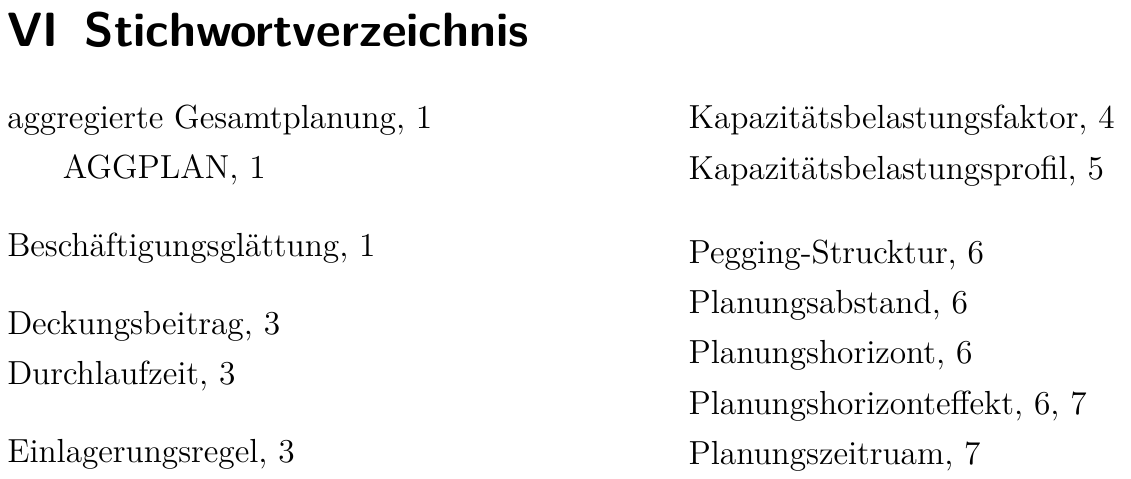
\includegraphics[width=0.7\linewidth]{Bilder/Stichwortverzeichnis}
    \caption{Stichwortverzeichnis mit Standardformatierung}
    \label{fig:Stichwortverzeichnis}
\end{figure}


\subsubsection{Stichwortverzeichnis mit eigener Formatierung}
Möchte man eine Formatierungsdatei mit angeben \glqq\_index.ist\grqq \ die im Ordner \glqq tex\grqq \ liegt würde der Befehl wie folgt aussehen.
\begin{lstlisting}
% WICHTIG!!!  
% Pseudokommentar um pdflatex zu erlauben andere Programme zu nutzen z.B. gnuplot
% !TeX TXS-program:compile = txs:///pdflatex/[--shell-escape] | makeindex.exe -g -s tex/_index.ist  %.idx | txs:///biber | txs:///pdflatex/[--shell-escape]
\end{lstlisting}
Mit dem Schalter -g kann MakeIndex die Daten nach DIN 5007-2 (deutsche Telefonbuchsortierung) sortieren. Allerdings muss dann mit Hilfe der Option -s auch eine eigene Stildatei eingebunden werden, da \grqq in MakeIndex standardmäßig eine andere Bedeutung besitzt. Wird das vergessen, erhält man die Fehlermeldung \glqq Option -g invalid, quote character must be different from \grq\grqq\grq.\grqq.
\begin{figure}[H]
\centering
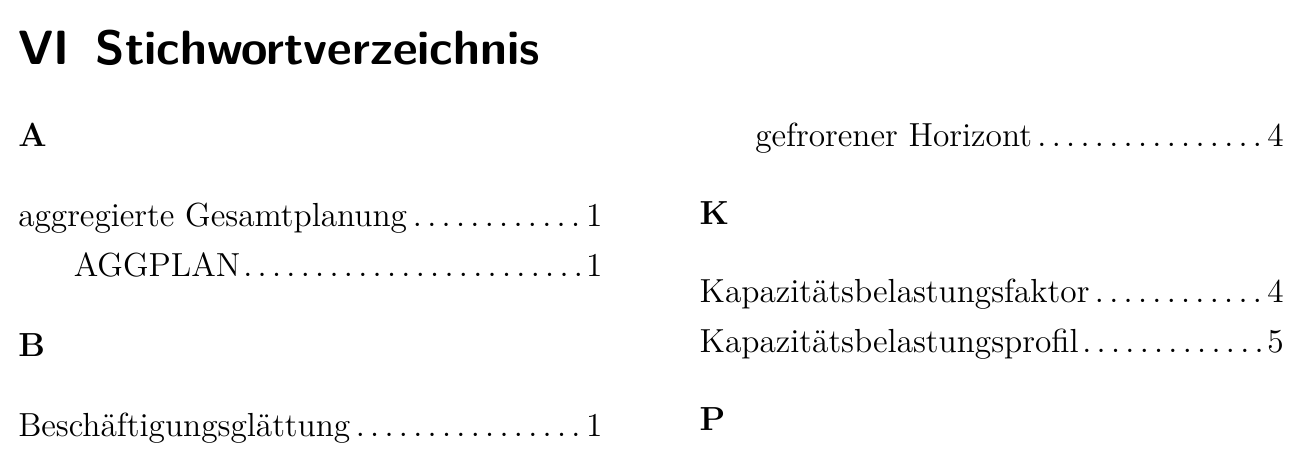
\includegraphics[width=0.7\linewidth]{Bilder/Stichwortverzeichnis_eigene_Formatierung}
\caption{Stichwortverzeichnis mit eigener Formatierung}
\label{fig:Stichwortverzeichnis_eigene_Formatierung}
\end{figure}


\subsubsection{Literaturverzeichnis mit biber immer erstellen}
Mit Hilfe des Pseudokommentars kann man auch einstellen, dass biber immer aufgerufen wird.
\begin{lstlisting}
% WICHTIG!!!  
% Pseudokommentar um pdflatex zu erlauben andere Programme zu nutzen z.B. gnuplot
% !TeX TXS-program:compile = txs:///pdflatex/[--shell-escape] | txs:///makeindex | txs:///biber | txs:///pdflatex/[--shell-escape]
\end{lstlisting}






\pagebreak

% ----------------------------------------------------------------------------------
% Anleitung wie eine Fallstudie aufgebaut ist
% ----------------------------------------------------------------------------------
\section{Einleitung}
\label{ch:einleitung}
In der Einleitung wird das Thema der Arbeit erläutert (z.B. Betrachtung der Durchlaufterminierung im \gls{MRP}).

Daraus ist die Fragestellung, die mit der Fallstudie bearbeitet wird, abzuleiten und zu begründen (z.B. Wie wirkt sich die Vorlaufzeit auf die Berechnung der Durchlaufterminierung aus?).

		\subsection{Rahmen}
		\label{ch:rahmen}
		Der Rahmen, indem die Fallstudie stattfindet, wird aufgezeigt (z.B.: Die Fallstudie entstand im Rahmen des Projektstudiums an der \gls{OTH} im \gls{LIP}). Damit wird der Umfang der erbrachten Arbeitszeit festgelegt und kann mit anderen, themenverwandten Fallstudien verglichen werden.

		\subsection{Voraussetzungen}
		\label{ch:vorraussetzungen}
		Die Voraussetzungen beschreiben das notwendige Arbeitsumfeld. Dazu gehören verwendete Werkzeuge mit Versionsständen, eventuell verwendete Vorlagen etc. (z.B. Für die Bearbeitung der Fallstudien wurde das laboreigene MRP-Werkzeug in Version 1.1.6 verwendet. Als Vorlage für die Fallstudie dient eine Ausarbeitung aus \cite{Herrmann.2009} S. 271 ff..)

		\subsection{Aufbau der Arbeit}
		\label{ch:Aufbau}
		Der Aufbau der Fallstudie (roter Faden) wird erläutert.

		\subsection{Eingliederung in den Produktionsprozess}
		In den Fallstudien, die im Rahmen des LIPs stattfinden, ist es sinnvoll, die erstellten Arbeiten in die Prozesskette des Vertriebs, der Produktion und der Beschaffung einzugliedern. Dazu werden die Darstellungen zur Produktionsplanung und -steuerung und dem Produktionsplanungsprozess nach \cite{Herrmann.2011} verwendet. Für diese Einordnung stehen nach den Ausführungen der Literatur die Darstellungen in den Abbildungen \ref{fig:gesamt} und \ref{fig:prozess} zur Verfügung. Im Bilder-Ordner dieser Vorlage ist ebenfalls das entsprechende Visio-File hinterlegt.

		\begin{figure}[H]
			\centering
			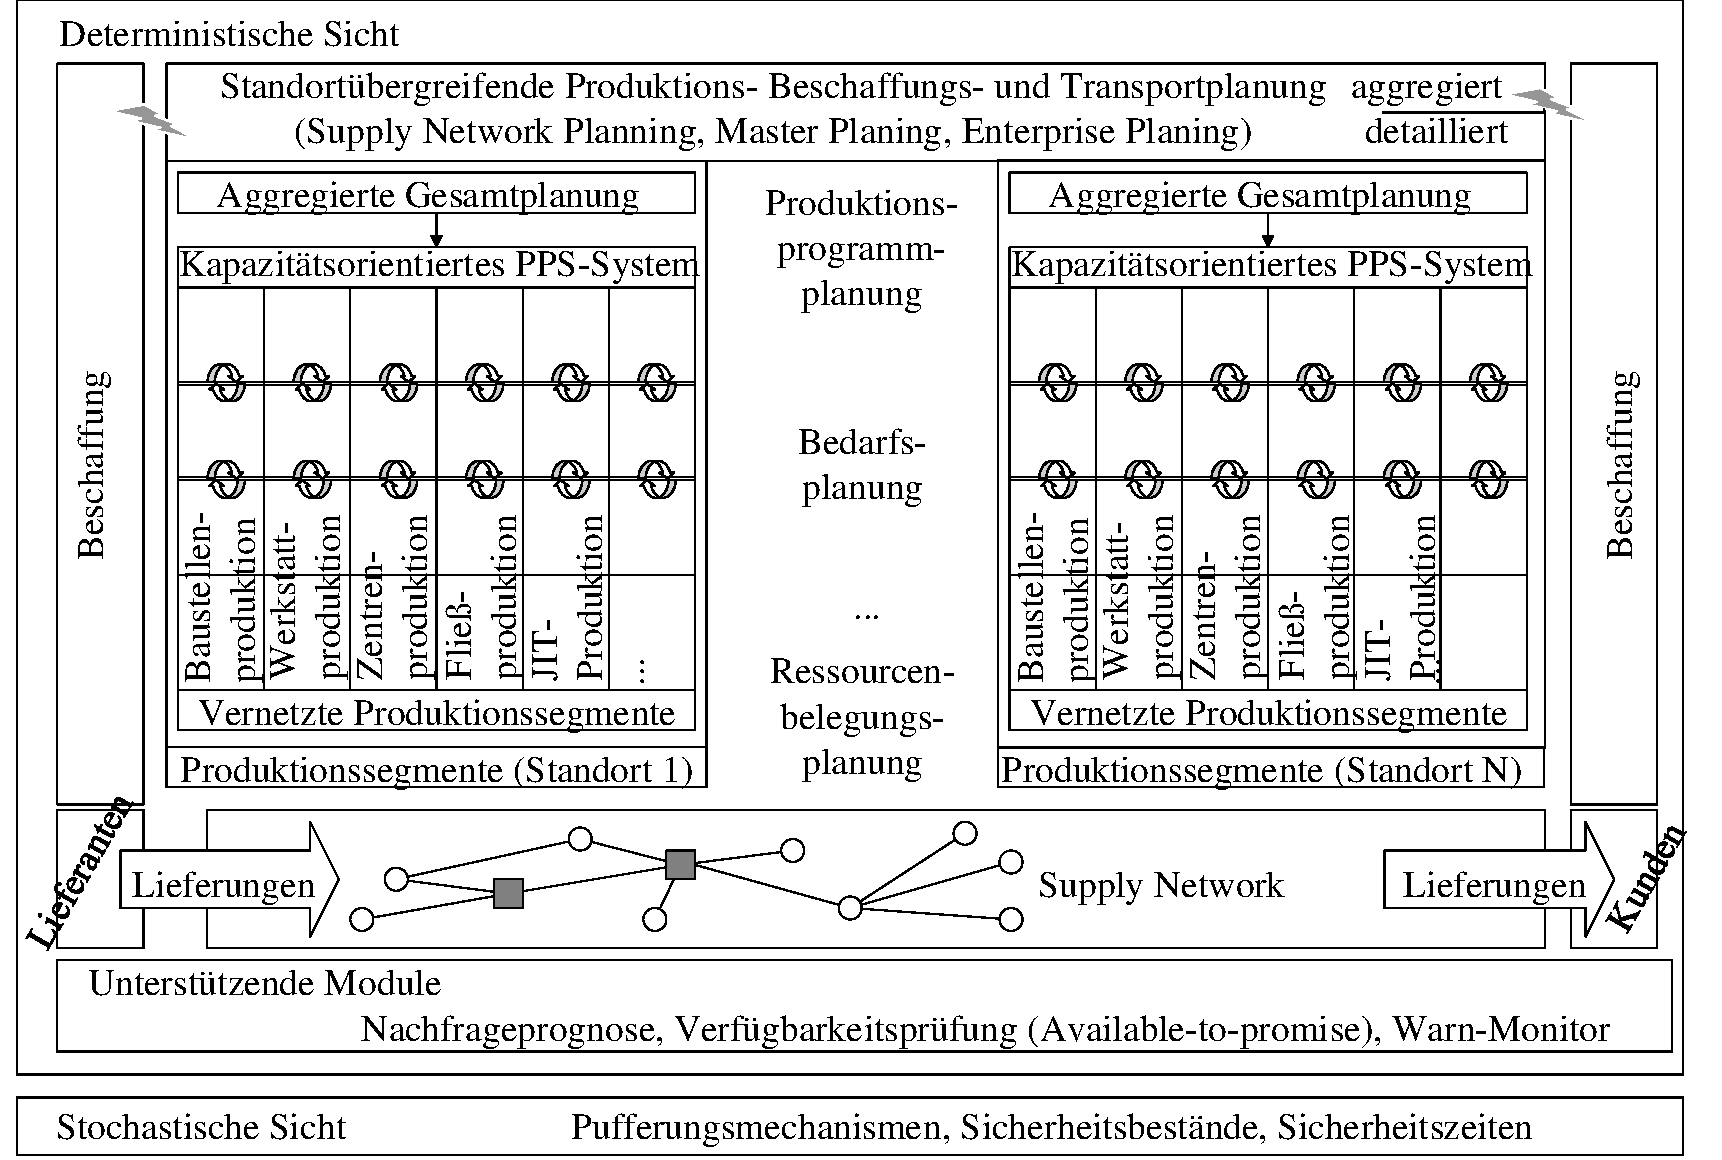
\includegraphics[width=0.8\linewidth]{Bilder/CGesamtuebersicht}
			\captionof{figure}{Produktionsplanung und -steuerung in der Industrie.}
			\label{fig:gesamt}
		\end{figure}

		Der Planungsprozess innerhalb eines PPS-Systems wird in der folgenden Darstellung detaillierter betrachtet.

		\begin{figure}[H]
			\centering
			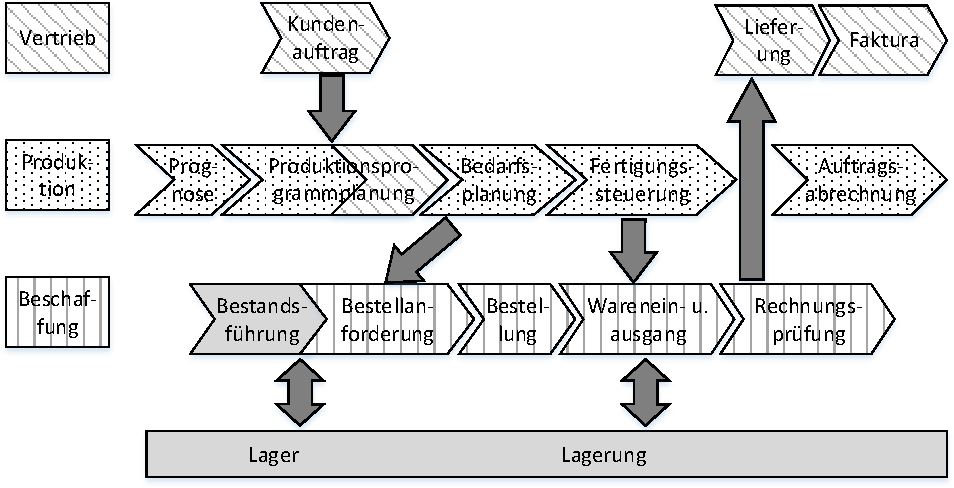
\includegraphics[width=0.8\linewidth]{Bilder/CProduktionsprogrammplanung}
			\captionof{figure}{Prozesskette zu Beschaffung, Produktion und Vertrieb \cite{Herrmann.2011}.}
			\label{fig:prozess}
		\end{figure}

		Für Fallstudien, die im Bereich der Bedarfsplanung angesiedelt sind, steht eine weitere Abbildung zur genaueren Einordnung, wie in Abbildung \ref{fig:bedarfsplanung} dargestellt, zur Verfügung. Auch hierzu ist die entsprechende Visio-Datei im Bilderordner zu finden.

		\begin{figure}[H]
			\centering
			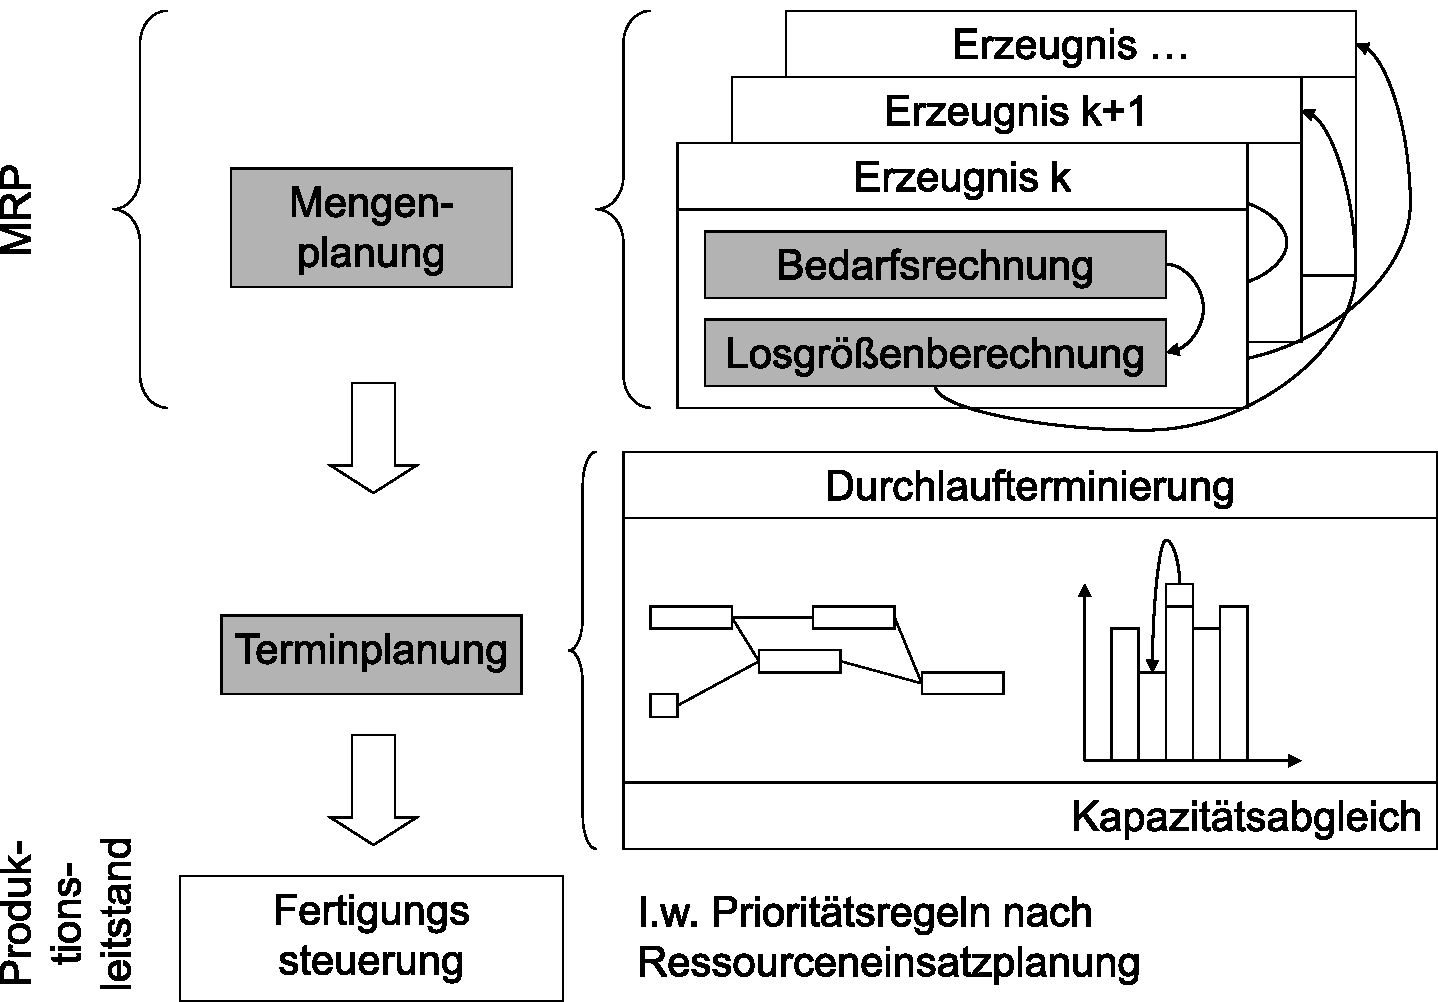
\includegraphics[width=0.8\linewidth]{Bilder/CLosgroessenplanung}
			\captionof{figure}{Prozesskette zu Beschaffung, Produktion und Vertrieb \cite{Herrmann.2011}.}
			\label{fig:bedarfsplanung}
		\end{figure}

		\pagebreak

		\section{Struktur der Studienarbeit}
		\label{ch:struktur}
		Vor allem in Abschlussarbeiten soll sich an folgender Struktur orientiert werden.
		\begin{enumerate}
            \item Was sind Ihre Kernergebnisse?
            \item Definieren Sie das Problem (z.B. Antwortzeiten von Kundenanfragen sind zu hoch).
            \item Analysieren Sie das Problem (im Hinblick auf die Prozesse und IT, z.B. Datenbankzeiten sind zu hoch).
            \item Erarbeiten Sie eine Lösung und setzen Sie diese um (z.B. bessere Select Statements).
            \item Evaluieren Sie die Güte der Lösung (z.B. Antwortzeiten wurden um 70\% reduziert).
        \end{enumerate}
		Entscheidend sind konkrete Aussagen, die quantitativ belegt werden.
		
		\vspace{\baselineskip}
		
		Bei der Analyse und Anwendung von Verfahren soll folgender Aufbau eingehalten werden:
		\begin{enumerate}
            \item Welches Problem wird gelöst? Dies ist an einem Beispiel aufzuzeigen.
            \item Wie wird das Problem gelöst?
            \begin{FHitemize}
            \item Algorithmus, Formeln usw. 
            \item Anwenden der Algorithmen, Formeln etc. auf das Beispiel.
        	\end{FHitemize}
        \end{enumerate}
       
        \vspace{\baselineskip}
         
		Bei der Ausarbeitung von Fallstudien soll sich an folgender Struktur orientiert werden:
		\begin{enumerate}
            \item Unternehmensbeschreibung mit allen Daten im Text. Dabei sind alle relevanten Daten zusätzlich in Tabellenform zusammenzufassen.
            \item Aufgabenstellung: diese ist kurz zu nennen.
            \item Lösung.
            \item Zusammenfassung: eventuell mit Anmerkungen zur Lösung, wie etwa Relevanz, Einsatz, Schwächen, Verbesserungsmöglichkeiten usw.
        \end{enumerate}
		\pagebreak



		\section{Beispiele für Ausarbeitungen}
		\label{ch:bsp-ausarbeitungen}

		In diesem Kapitel sind Beispiele aufgeführt, die Teile dieser Vorlage exemplarisch darstellen sollen.\\
		Beispiele 1 stellt die graphische Lösung eines linearen Optimierungsproblems dar. Die Abbildung wurde dazu mit Ti\textit{k}Z erstellt.\\
		Beispiel 2 zeigt die Darstellung des Optimierungsmodells CLSP. Dabei wird das Einbinden von Listings exemplarisch aufgezeigt.
		
		\subsection{Graphische Lösung eines linearen Optimierungsmodells, Beispiel 1}
				
		Gegeben ist das folgende lineare Optimierungsproblem:

		Variablen:
		\begin{tabularx}{\linewidth}{@{}p{2 cm}X}  %wichtig \keepXColumns muss gesetzt sein 
            $x_1 \in \mathbb{R} $&  \\
            $x_2 \in \mathbb{R} $ &  \\
		\end{tabularx}

		Maximiere F($x_1$,$x_2$) = $ 2 \cdot x_{1} + 5 \cdot x_{2}  $ \\
		s.t.

		\begin{tabularx}{\linewidth}{@{}p{5 cm}X}  %wichtig \keepXColumns muss gesetzt sein
			$4 \cdot x_{1} + x_2  \le 26 $					& (1) \\
			$x_1 + 4 \cdot x_{2} \le 24 $   				& (2) \\
			$3 \cdot x_{1} + 2 \cdot x_{2} \le 22 $  		& (3) \\
			$x_1 \geq 0$									& (4) \\ 
			$x_2 \geq 0$									& (5) \\
		\end{tabularx}

		Lösen Sie dieses lineare Optimierungsproblem nach dem graphischen Verfahren.\\


		\minisec{Lösung}

		Die graphische Darstellung zu diesem linearen Optimierungsproblem ist in der folgenden Abbildung \ref{fig:LinOpt-Graph-Bsp1} angegeben.

		\begin{figure}[H]
		\centering
			
		\begin{tikzpicture}[scale=1] %wenn scale=2, dann ergänze: font=\tiny

		
		\node[yshift=-0.265cm] at (0:0){0};	% Beschriftung Nullpunkt	
		
		\begin{axis}[
		width=14cm, height=14cm, %Größe der Abbildung
		axis lines=middle,
		axis equal,
		axis line style={-latex}, %Pfeil bei Achse nur in eine Richtung, ansonsten {latex-latex}
		%x-Achse:%		
			domain=-26:26, %x-Achsen-Bereich, in dem Plots dargestellt werden können
			smooth,
			xmin=-0.20,xmax=26.9, %Bereich der x-Achse
			tick style={line width=.5pt,black},	tick label style={fill=white},
			xtick={0, 2, 4, ..., 26}, xlabel=$x_1$, xlabel style={right,inner xsep=2pt}, %x-Achsenbeschriftung   	
      		%extra x ticks={0.5},extra x tick labels={0.5}, %Beschriftung von x-Koordinate 0,5
      	%y-Achse:%
      		restrict y to domain=-26:27.1, %y-Achsen-Bereich, in dem Plots dargestellt werden können
      		ymin=-0.20,ymax=26.9, %Bereich der y-Achse
      		ytick={0,2, 4, ..., 26}, ylabel=$x_2$, ylabel style={above,inner ysep=2pt},  %y-Achsenbeschriftung  
      		%extra y ticks={0.5},extra y tick labels={0.5}, %Beschriftung von y-Koordinate 0,5
      	%minor tick num=4, minor tick length=4pt, minor tick style={line width=.5pt}, %Teilstriche x- und y-Achse
      	samples=100, %Punkte je Plot
    	]
		
		
		%Lösungsraum:%
		\addplot[pattern=north east lines,pattern color=black!50] (0,0) -- (6.5,0) -- (6,2) -- (4,5)-- (0,6)\closedcycle; %Lösungsraum
			%\node at (0.8,2.85) {Lösungsraum}; %Beschriftung Lösungsraum
		
		%Gleichung 1:%		
		\addplot[black] {(-4)*x + 26}; %Gleichung 1: 4x1 + x2 <= 26
			\node at (2.3,20) {(1)};
			%Koordinaten für Richtungspfeil "oben-rechts" für Gleichung 1:
				\coordinate (a) at (2,18);
				\coordinate (b) at ($ (2,18)!0.45cm!-90:(4,10) $);
			%Koordinaten für Richtungspfeil "unten-links" für Gleichung 1:	
				\coordinate (c) at (4,10);
				\coordinate (d) at ($ (4,10)!0.45cm!-90:(5,6) $);
			%Richtungspfeile für Gleichung 1:	
			\draw[>=Straight Barb,->] (a) -- (b);
			\draw[>=Straight Barb,->] (c) -- (d);		


		%Gleichung 2:%
		\addplot[black] {(-0.25)*x + 6}; %Gleichung 2: x1 + 4x2 <= 24
		\node at (14,3.5){(2)};
			%Koordinaten für Richtungspfeil "oben-rechts" für Gleichung 2:
				\coordinate (i) at (2,5.5);
				\coordinate (j) at ($ (2,5.5)!0.45cm!-90:(3,5.25) $);  %% 
			%Koordinaten für Richtungspfeil "unten-links" für Gleichung 2:
				\coordinate (k) at (10,3.5);
				\coordinate (l) at ($ (10,3.5)!0.45cm!-90:(12,3) $);
			%Richtungspfeile für Gleichung 2:	
			\draw[>=Straight Barb,->] (i) -- (j);
			\draw[>=Straight Barb,->] (k) -- (l);	

		%Gleichung 3:%
		\addplot[black] {(-1.5)*x + 11} ; %Gleichung 3: 3x1 + 2x2 <= 22
			\node at (2.2,9) {(3)}; %Beschriftung Gleichung 3
			%Koordinaten für Richtungspfeil "oben-rechts" für Gleichung 3:
				\coordinate (e) at (2,8);
				\coordinate (f) at ($ (2,8)!0.45cm!-90:(4,5) $);  %% 
			%Koordinaten für Richtungspfeil "unten-links" für Gleichung 3:
				\coordinate (g) at (5,3.5);
				\coordinate (h) at ($ (5,3.5)!0.45cm!-90:(6,2) $);
			%Richtungspfeile für Gleichung 3:	
			\draw[>=Straight Barb,->] (e) -- (f);
			\draw[>=Straight Barb,->] (g) -- (h);		

	
		
		%Gleichung 4:%		
		\draw [black] (0,0) -- (0,26); %Gleichung 4: x1 >= 0;	
			\node at (0.75, 14.25){(4)};
			%i, j	
			\coordinate (i) at (0,1);	
			\coordinate (j) at ($ (i)!0.45cm!-90:(0,13.5) $);
			\coordinate (k) at (0,13.5);
			\coordinate (l) at ($ (k)!0.45cm!90:(0,1) $);
			\draw[>=Straight Barb,->] (i) -- (j);
			\draw[>=Straight Barb,->] (k) -- (l);
		
		%Gleichung 5:%			
		\addplot[black] {0}; %Gleichung 5: x2 >= 0
			\node at (13,0.75){(5)};
			%m,n,o,p
			\coordinate (m) at (9,0);	
			\coordinate (n) at ($ (m)!0.45cm!90:(16.5,0) $);
			\coordinate (o) at (16.5,0);
			\coordinate (p) at ($ (o)!0.45cm!-90:(9,0) $);
			\draw[>=Straight Barb,->] (m) -- (n);
			\draw[>=Straight Barb,->] (o) -- (p);
			
			
			%%\draw[>=Straight Barb,->](9,0)--(9,1)node{}; %Richtungspfeil für Gleichung 5			
			%\draw[>=Straight Barb,->](16.5,0)--(16.5,1)node{}; %Richtungspfeil für Gleichung 5
	
		
		%Gleichung ZF:%
		\addplot[black, dashed] {(-0.4)*(x-6)} ; %Zielfunktion: Maximiere 2x1 + 5x2  %x-shift in Höhe von 6 zur Darstellung in Koordinatensystem%
			\node at (3.8,1.55) {(ZF)}; %Beschriftung Zielfunktion
			
			%Koordinaten für Richtungspfeil Gleichung ZF:
				\coordinate (q) at (2,1.6); %Pfeil beginnt bei x=2 und y=(-0.4*(2-5.5))=1.4
				\coordinate (r) at ($ (2,1.6)!0.45cm!90:(3,1.2) $);  %Pfeil als Orthogonale zwischen Punkt i und Punkt j (x=3; y=(-0.4*(3-5.5))=1)
				
			%Richtungspfeile für Gleichung ZF:	
				\draw[>=Straight Barb,->] (q) -- (r);
								
		\draw[black](4,5)circle[radius=3pt];%Optimaler Punkt
			\node at (4.35,5.7) {OP};
		\end{axis}
		
		%%Legende		
		\node at (-0.2,-1.5)[label=right: OP: Optimaler Punkt;\quad    ZF: Zielfunktion;]{};
		\node[draw, minimum width=0.7cm,minimum height=0.3cm,pattern=north east lines,pattern color=black!50](Legend) at (8.6,-1.5)[label=right: Lösungsraum]{}; 		
		
		\end{tikzpicture}
		\captionof{figure}{Graphische Darstellung zum linearen Optimierungsproblem (Beispiel 1).}
		\label{fig:LinOpt-Graph-Bsp1}
		\end{figure}

		Nach dem graphischen Lösungsverfahren wird nun die Zielfunktion (ZF) in Richtung steigender Zielfunktionswerte (d.h. nach oben) verschoben. Der letzte Punkt vor dem Verlassen des Lösungsraums ist der in der Abbildung \ref{fig:LinOpt-Graph-Bsp1} 				eingezeichnete und mit „OP“ markierte Punkt. Es handelt sich um den Schnittpunkt der Restriktionen (2) und (3). Dies bestimmt das folgende lineare Gleichungssystem: \\

		$\hspace*{5,4mm}
		\begin{bmatrix}
			x_{1} & + & 4x_{2} &= & 24  \\
			3x_{1} & + & 2x_{2} &= & 22 
		\end{bmatrix}
		\begin{matrix}
			\  (2) \\
			\  (3) 
		\end{matrix}
		$ \\ 
		
		Seine Lösung durch das Gaußsche Eliminationsverfahren führt zu den folgenden Äquivalenzumformungen: \\

		$\Leftrightarrow
		\begin{bmatrix}
	 		x_{1}  &  + & 4x_{2}  &= &  24  \\
			&  - & 10x_{2} &= & -50 
		\end{bmatrix}
		\begin{matrix}
			& \ | \ (2)  \\
			\text{durch } (3) - 3 \cdot (2)	& \ | \ (3)
		\end{matrix}$ \\ \\

		$\Leftrightarrow
		\begin{bmatrix}
			x_{1} &  + & 4x_{2} & = & 24  \\
			  &    & x_{2}  &= & 5 	
		\end{bmatrix}
		\begin{matrix}
			& \ | \ (2)  \\
		\text{durch } (3) : (-10)	& \ | \ (3)
		\end{matrix}$ \\ \\

		$\Leftrightarrow
		\begin{bmatrix}
			x_{1} &  + & 4 \cdot 5 & = & 24  \\
			&   & x_{2}  &= & 5 	
		\end{bmatrix}
		\begin{matrix}
			\text{durch Einsetzen von } \ x_2 = 5 & \ | \ (2) \\
			& \ | \ (3)  \\
		\end{matrix}$ \\ \\

		$\Leftrightarrow
		\begin{bmatrix}
			x_1 & & & = & 4 \\
			& & x_2 & = & 5 
		\end{bmatrix}
		\begin{matrix}
			\ \text{durch Umformen von} \ (2)   \\
			& 
		\end{matrix}$\\

		Durch das Lösen des linearen Gleichungssystems wurde somit ermittelt, dass $(4,5)$ der optimale Punkt ist. Durch Einsetzen in die Zielfunktion ergibt sich $2 \cdot 4 + 5 \cdot 5$
		und damit der optimale, d.h. größte Wert, von 33. \\
		
		
		\subsection{Capacitated Lotsizing Problem (CLSP), Beispiel 2}
		Das lineare Optimierungsmodell \textbf{C}apacitated \textbf{L}ot\textbf{s}izing \textbf{P}roblem (CLSP) wird im Folgenden komprimiert dargestellt.\\ 
		Für Details sei auf \cite{Herrmann.2009} verwiesen. \\

		Parameter: 
		%\begin{table}[H]
		\begin{longtable}{ l l }
			T & Länge des Planungszeitraums $(1 \le t \le T)$ \\
			K & Anzahl der Produkte $(1 \le k \le K)$ \\
			J & Anzahl der Ressourcen $(1 \le j \le J)$ \\
			M & große Zahl (mindestens so groß wie größtmögliche Lösgröße) \\
			$b_{j,t}$ & verfügbare Kapazität der Ressource j in Periode t $\forall\; 1 \le j \le J$ und $1 \le t \le T$ \\
			$d_{k,t}$ & Nettobedarfsmenge des Produkts k in Periode t $\forall\; 1 \le k \le K$ und $1 \le t \le T$ \\
			$h_{k}$ & Lagerkostensatz für Produkt k $\forall\; 1 \le k \le K$ \\
			$s_{k}$ & Rüstkostensatz für Produkt k $\forall\; 1 \le k \le K$ \\
			$tb_{k,j}$ & Bearbeitungszeit für eine Einheit von Produkt k an Ressource j $\forall\; 1 \le k \le K$ \\
			& und $1 \le j \le J$\\
			$tr_{k,j}$ & Rüstzeit für Produkt k an Ressource j $\forall\; 1 \le k \le K$  und $1 \le j \le J$ \\
			$z_{k}$ & Mindestvorlaufzeit eines Auftrags für Produkt k $\forall\; 1 \le k \le K$\\
			$LA_{k}$ & Anfangslagerbestand für Produkt k $\forall\; 1 \le k \le K$ 
		\end{longtable}
		%\end{table}
		\addtocounter{table}{-1} % Herausnehmen dieser Tabelle aus dem Zähler
		
		Variablen: 
		%\begin{table}[H]	%Beginn der Tabelle; [H] setzt die Tabelle an die aktuelle Cursorposition
		\begin{longtable}{ l l}
			$q_{k,t}$ & Losgröße des Produkts k in Periode t $\forall\; 1 \le k \le K$ und $1 \le t \le T$ \\
			$y_{k,t}$ & Lagerbestand für Produkt k am Ende der Periode t $\forall\; 1 \le k \le K$ und $0 \le t \le T$ \\
			$\gamma_{k,t}$ & binäre Rüstvariable für Produkt k in Periode t mit $\gamma_{k,t}$ =  $\begin{cases}1&\text{falls $q_{k,t}$ $\textgreater$ 0}\\0&\text{falls $q_{k,t}$ = 0}\end{cases}$ \\
			& $\forall$ 1 $\le$ k $\le$ K und $1 \le t \le T$ 
		\end{longtable}
		%\end{table} 
		\addtocounter{table}{-1} % Herausnehmen dieser Tabelle aus dem Zähler

		\begin{fleqn}
		\begin{align*}
			\text{min} ~ \sum\limits_{k = 1}^K\sum\limits_{t = 1}^T(s_{k}\cdot \gamma_{k,t} + h_{k}\cdot y_{k,t})
		\end{align*}
		\end{fleqn}

		unter den Restriktionen \\
		$y_{k,t-1} + q_{k,t-z_{k}} -  d_{k,t} = y_{k,t}$ $\forall\; 1 \le k \le K$ und $1 \le t \le T$ \hfill Lager-
		\begin{flushright}
		bilanzgleichungen
		\end{flushright}
		$q_{k,t} - M \cdot \gamma_{k,t} \le 0$ $\forall\; 1 \le k \le K$ und $1 \le t \le T$ \hfill Rüstbedingung \\
		%$M_{k,j,t} = min  \left\{ \frac{b_{j,t}}{tb_{k,j}}, \sum\limits_{i = t}^T d_{k,i} \right\}$ & $\forall\; 1 \le k \le K$ und $1 \le j \le J$ und $1 \le t \le T$ \\
		$\sum\limits_{k = 1}^K(tb_{k,j}\cdot q_{k,t} + tr_{k,j}\cdot \gamma_{k,t})\le b_{j,t}$ $\forall\; 1\le j \le J$ und $1 \le t \le T$ \hfill Kapazitätsrestriktion \\
		$y_{k,0} = 0,\; y_{k,T} = 0 $ $\forall\; 1 \le k \le K$ \hfill Lageranfangs- und endbestand \\
		$q_{k,t},\;  y_{k,t} \;\ge\; 0$ $\forall\; 1 \le k \le K$ und $1 \le t \le T$ \hfill Nicht- \\
		$\gamma_{k,t} \in \{0, 1\}$ $\forall\; 1 \le k \le K$ und $1 \le t \le T$ \hfill negativität. \\


		Die Umsetzung dieses Optimierungsproblems in ILOG lautet -- als „mod“-Datei:\\
		\lstinputlisting[label=lst:CLSP,captionpos=b,caption=Implementierung vom Modell CLSP in ILOG.]{Listing/CLSP.mod}


		Die Parameter für das konkrete Zahlenbeispiel lauten -- als „dat“-Datei (zur Vereinfachung sind nicht alle 12 Perioden vor dem Planungsintervall angegeben, sondern nur einige, um eine Vorproduktion zu erlauben):\\ 
		\lstinputlisting[label=lst:CLSPD,captionpos=b,caption=Implementierung ILOG Parameter beim Schuhproduzenten.]{Listing/CLSP_Schuhproduzent.dat} 

		\pagebreak
		%-------------------------------------------------------------------------------------
		% Verzeichnisse %-------------------------------------------------------------------------------------
		\rhead{Verzeichnisse} %Kopftextbeschriftung

		\stepcounter{section}
		\phantomsection \label{Verzeichnisse}
		\addcontentsline{toc}{section}{Verzeichnisse} %Ohne Nummer ins Inhaltsverzeichnis
		\renewcommand{\thesection}{\Roman{verzeichnis}}
		\section*{Verzeichnisse}
		% Literaturverzeichnis
		\rhead{Verzeichnisse}
   		\phantomsection \label{Literaturverzeichnis}
		\renewcommand{\refname}{Literaturverzeichnis}
		\printbibliography
		\pagebreak

		% Abbildungsverzeichnis
		\stepcounter{verzeichnis}
		\listoffigures
		\pagebreak

		% Tabellenverzeichnis

		\stepcounter{verzeichnis}
		\listoftables
		\pagebreak

        % Listingverzeichnis
        \stepcounter{verzeichnis}
        \lstlistoflistings
        \pagebreak

        % Algorithmusverzeichnis
        %\renewcommand{\listalgorithmname}{Algorithmenverzeichnis}
        %\listofalgorithms
        \stepcounter{verzeichnis}

        \section{Algorithmenverzeichnis}
        \vspace{-2em}
        \listoftoc[]{loa}



% Stichwortverzeichnis
\pagebreak
\stepcounter{verzeichnis}
% Stichwortverzeichnis soll im Inhaltsverzeichnis auftauchen
\section{Stichwortverzeichnis}

% Abstand analog der anderen Verzeichnisse reduzieren
\vspace{-3em}

% Stichwortverzeichnis endgueltig anzeigen

\printindex

		% Abkürzungen
        \pagebreak
		\stepcounter{verzeichnis}
		\section{Abkürzungsverzeichnis}
		\vspace{-4em} % Abstand analog der anderen Verzeichnisse reduzieren
		\printnoidxglossary[type=\acronymtype,style=alttree,title=,toctitle=] %automatischen Titel und Gliederungsbeschriftung unterdrücken - sonst steht da Glossarie
		%\printglossary[type=\acronymtype,style=alttree,title=,toctitle=] %automatischen Titel und Gliederungsbeschriftung unterdrücken - sonst steht da Glossarie
		\newpage

		% ---------------------------------------------------------------------------------
		% Anhang
		% ---------------------------------------------------------------------------------
		\rhead{Anhang}        %Kopftextbeschriftung
		\begin{appendix}
			\phantomsection \label{Anhang}
			\section*{Anhang}\addcontentsline{toc}{section}{Anhang} %Anhang ohne Nummer
			\renewcommand{\thesection}{\Roman{section}}

			\setcounter{section}{0} %Counter für Nummerierung der Anhänge initalisieren
			\section{Remotenutzung der CIP-Pool-Rechner}
			\label{app:remotenutzung}
			Für die Remotenutzung der CIP-Pool-Rechner sind folgende Schritte zu vollziehen. \\
			Es sei angemerkt, dass nach aktuellem Stand (09.12.2020) die CIP-Pool-Rechner bis März 2021 zur Remotenutzung zur Verfügung stehen.
			
			\begin{enumerate}
				\item Eine Verbindung mit dem Hochschulnetz muss aufgebaut werden. Dies ist mittels VPN (siehe \href{https://www.oth-regensburg.de/supportwiki/doku.php?id=public:netz:vpn-forticlient}{\underline{Anleitung}}) möglich.
				
				\item Die Seite \url{https://remote-cip-wa.hs-regensburg.de/RDWeb/} muss aufgerufen werden. \\
				Im Anschluss muss die Anmeldung mittels NDS-Kennung im Format \textbf{HSR\textbackslash}abc12345 erfolgen.
				
					\begin{figure}[H]
      				\centering
        			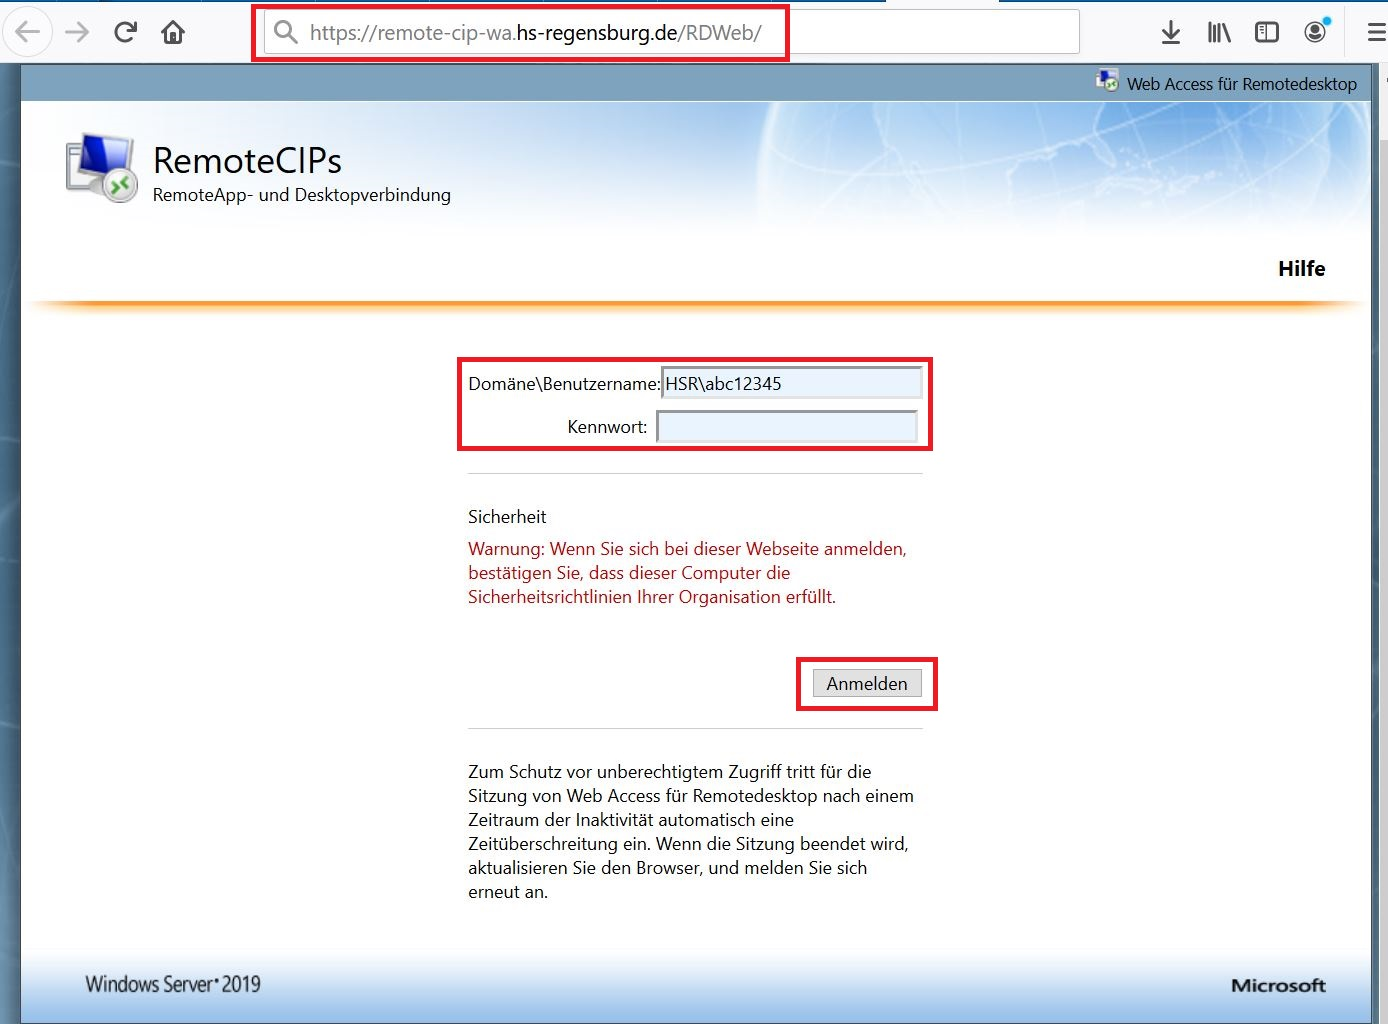
\includegraphics[width=1\textwidth]{Bilder/201209_Remote1}
        			\caption{CIP-Pool-Remotenutzung: Anmeldung auf Website}
        			\label{fig:201209_Remote1}
        			\end{figure}				
				\smallskip
				\item Nach erfolgter Anmeldung ist durch einen Mausklick der CIP-Pool auszuwählen, dessen Rechner man nutzen möchte. In dieser Anleitung wird der CIP-Pool der Maschinenbau-Fakultät ausgewählt.
				
					\begin{figure}[H]
      				\centering
        			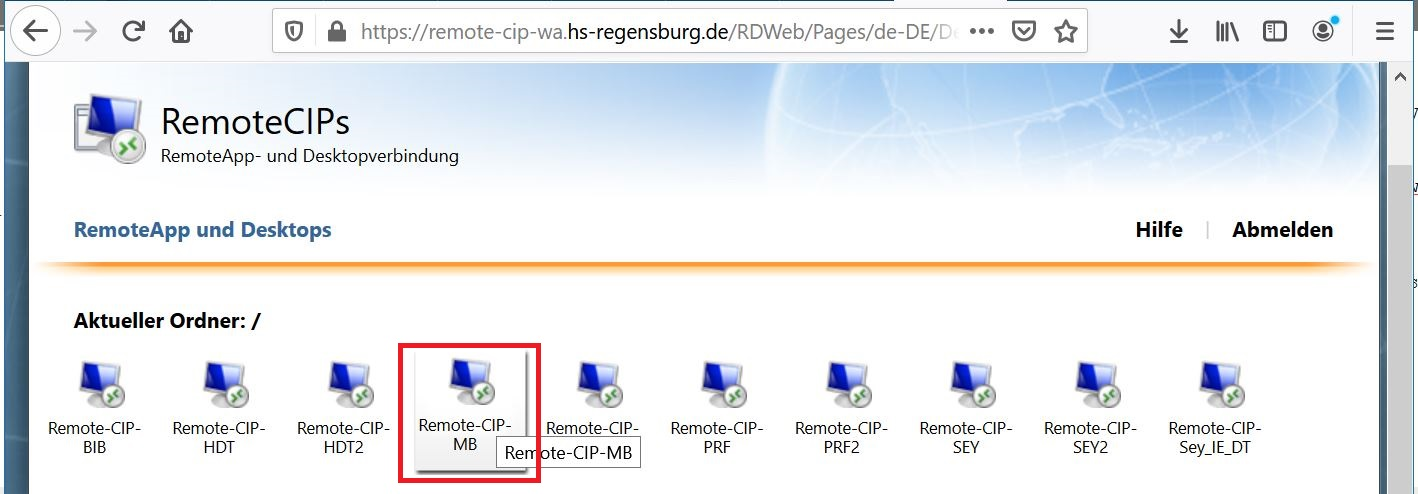
\includegraphics[width=1\textwidth]{Bilder/201209_Remote2}
        			\caption{CIP-Pool-Remotenutzung: Auswahl des CIP-Pools}
        			\label{fig:201209_Remote2}
        			\end{figure}
				
				\item Die aufkommende Meldung ist zu bestätigen. Es wird ein Öffnen mit der Standardanwendung empfohlen.

					\begin{figure}[H]
      				\centering
        			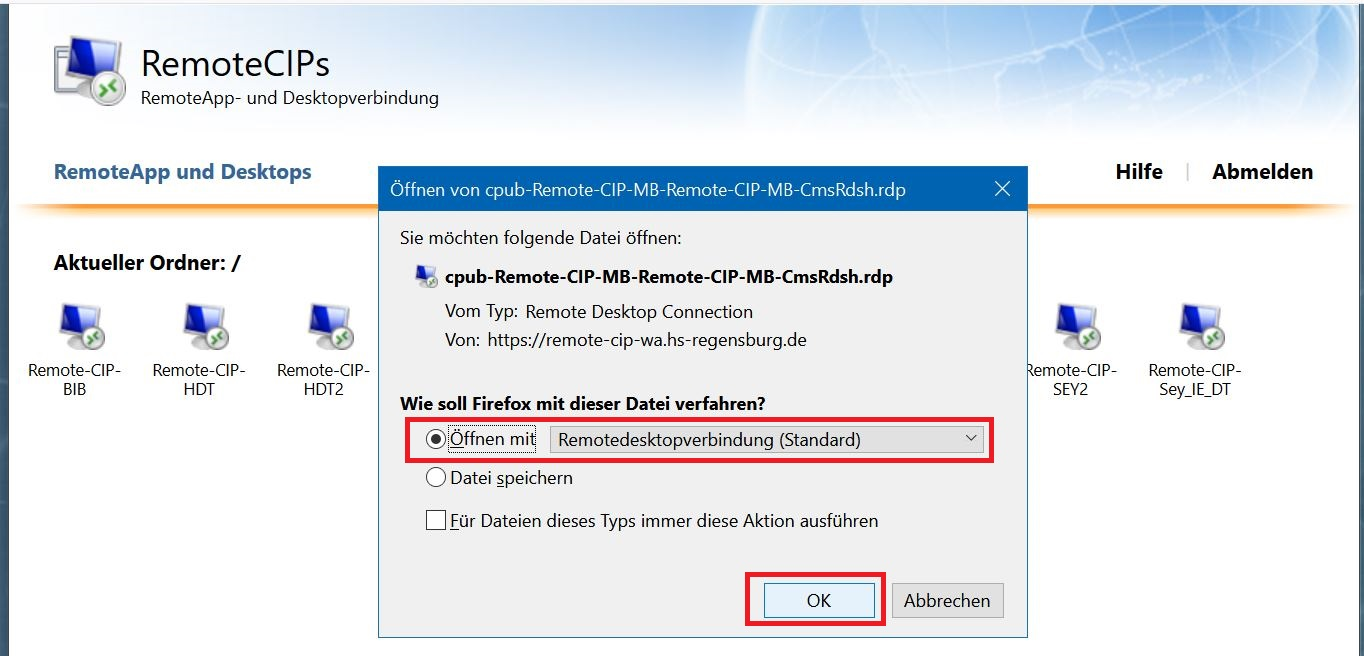
\includegraphics[width=1\textwidth]{Bilder/201209_Remote3}
        			\caption{CIP-Pool-Remotenutzung: Öffnen der Anwendung zur Remote Desktop Connection}
        			\label{fig:201209_Remote3}
        			\end{figure}				
				\medskip
				\item Die aufkommende Meldung ist durch Klicken auf \glqq Verbinden\grqq{} zu bestätigen.

					\begin{figure}[H]
      				\centering
        			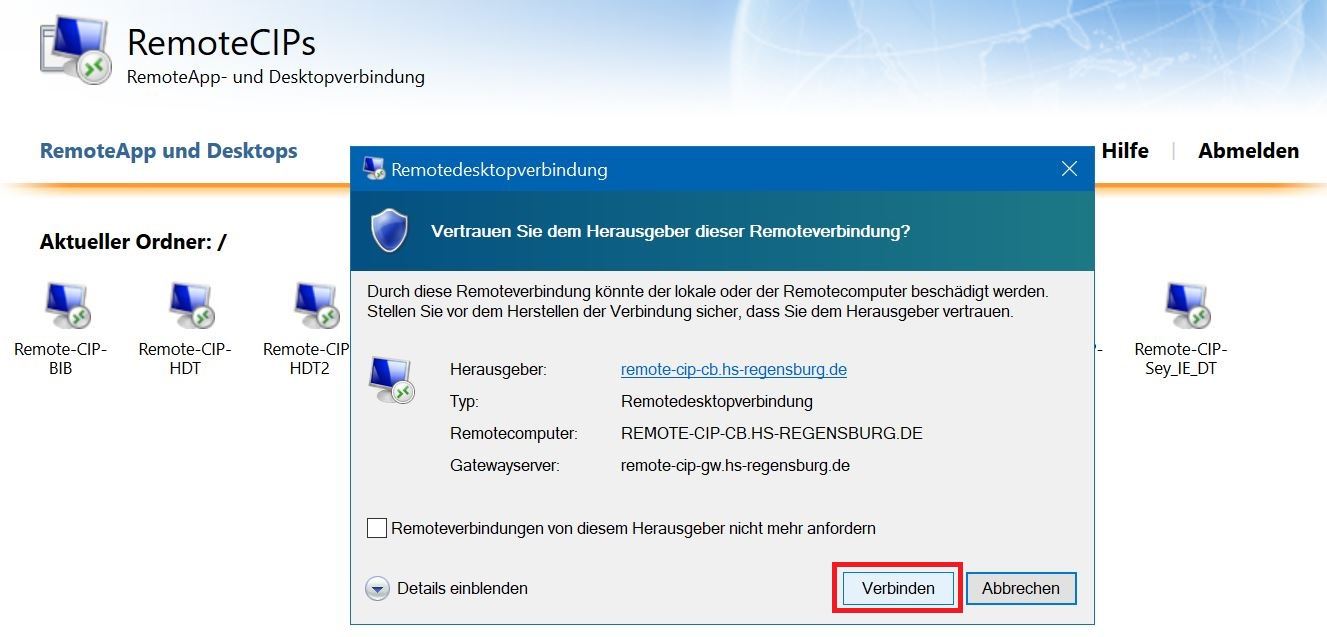
\includegraphics[width=1\textwidth]{Bilder/201209_Remote4}
        			\caption{CIP-Pool-Remotenutzung: Bestätigen der Verbindung}
        			\label{fig:201209_Remote4}
        			\end{figure}				
				
				\item Bevor der CIP-Rechner nun genutzt werden kann, muss erneut eine Anmeldung mittels NDS-Kennung im Format \textbf{HSR\textbackslash}abc12345 erfolgen.
				
					\begin{figure}[H]
      				\centering
        			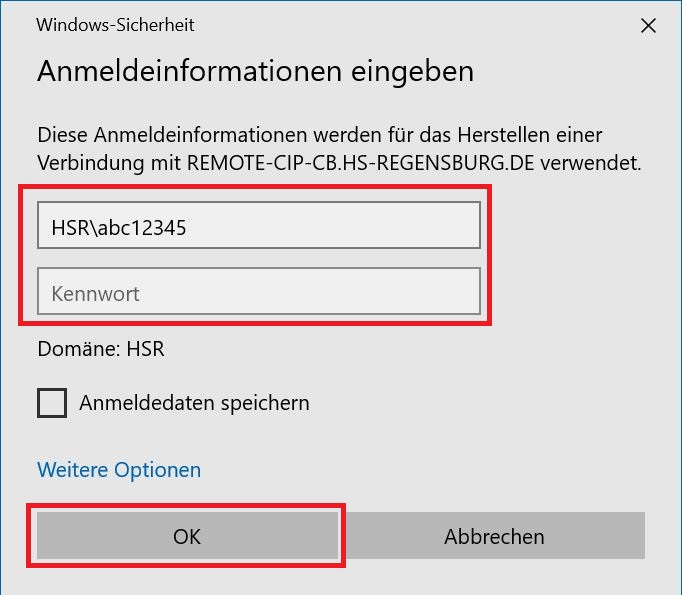
\includegraphics[height=0.3\textheight]{Bilder/201209_Remote5}
        			\caption{CIP-Pool-Remotenutzung: erneute Anmeldung}
        			\label{fig:201209_Remote5}
        			\end{figure}				
				\medskip
				\item Wenn der CIP-Rechner nicht mehr benötigt wird, ist eine Abmeldung des Benutzers durchzuführen.
				
					\begin{figure}[H]
      				\centering
        			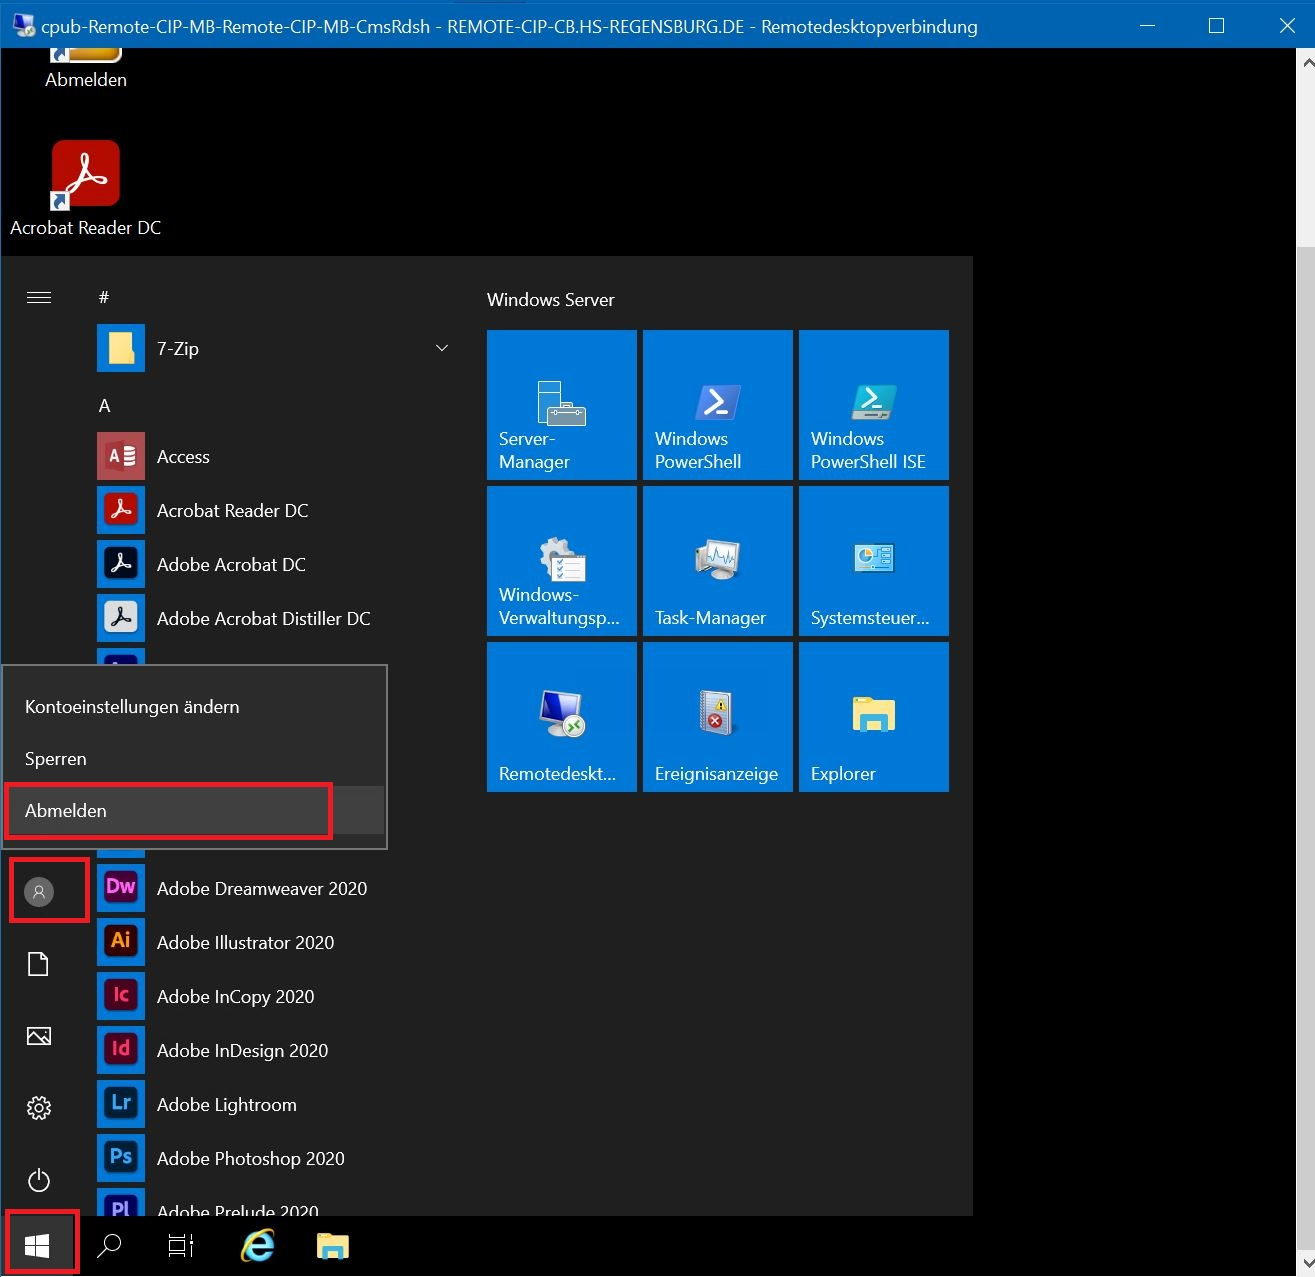
\includegraphics[width=1\textwidth]{Bilder/201209_Remote6}
        			\caption{CIP-Pool-Remotenutzung: Abmeldung des Benutzers}
        			\label{fig:201209_Remote6}
        			\end{figure}				
				
			\end{enumerate}	
			
			
		\end{appendix}


\section{Einleitung}
\label{sec:einleitung}

Aluminium ist ein wichtiger Rohstoff in vielen Industriezweigen, darunter die Automobilbranche, Bau- und Verpackungsindustrie. Die Preisentwicklung von Aluminium ist von großer Bedeutung für Unternehmen, die diesen Rohstoff verwenden, da sie direkte 
Auswirkungen auf die Produktionskosten und die Wettbewerbsfähigkeit haben kann. Beispielsweise können steigende Aluminiumpreise die Gewinnmargen von Unternehmen verringern, während sinkende Preise die Rentabilität verbessern können. Daher ist es für Unternehmen von entscheidender Bedeutung, die zukünftige Preisentwicklung von Aluminium vorherzusagen, um fundierte Entscheidungen treffen zu können. Eine Preisveränderung kann durch verschiedene Faktoren beeinflusst werden, wie z.B. Angebot und Nachfrage, geopolitische Ereignisse, wirtschaftliche Entwicklungen und technologische Fortschritte. Daher ist die Fähigkeit, die zukünftige Preisentwicklung von Aluminium vorherzusagen, von großem Interesse für Unternehmen und Investoren.

\paragraph{Schwierigkeit des Projektes}
Die Schwierigkeit des Projektes liegt darin, dass die Preisentwicklung von Aluminium von einer Vielzahl von Faktoren beeinflusst wird, die oft komplex und miteinander verknüpft sind. Beispielsweise können geopolitische Ereignisse wie Handelskonflikte oder Naturkatastrophen die Produktion und den Handel von Aluminium beeinträchtigen, was zu plötzlichen Preisänderungen führen kann. Darüber hinaus können wirtschaftliche Entwicklungen wie Inflation oder Wechselkursschwankungen die Nachfrage nach Aluminium beeinflussen, was ebenfalls Auswirkungen auf die Preise haben kann. Somit sind nicht nur datenbasierte Komponenten relevant, sondern regelbasierte Ansätze können ebenfalls von Bedeutung sein, um die Preisentwicklung von Aluminium zu modellieren und vorherzusagen.

\paragraph{Motivation und Ziel}
Die Motivation des Projektes besteht darin, ein Muster in den historischen Preisdaten zu erkennen und diese Informationen zu nutzen, um zukünftige Preisbewegungen vorherzusagen. Mehrere Ansätze können verwendet werden, um dieses Ziel zu erreichen, darunter Zeitreihenanalyse, maschinelles Lernen und statistische Modelle. Der gewählte Ansatz für dieses Projekt ist die Anwendung von Zeitreihenanalyse und maschinellem Lernen, um die Preisentwicklung von Aluminium zu modellieren und vorherzusagen. Hierzu werden zunächst die Rohdaten gesammelt und aufbereitet, um sie für die Analyse nutzbar zu machen. Anschließend werden verschiedene Modelle getestet und verglichen, um die beste Vorhersagegenauigkeit zu erzielen. Das Ziel des Projekts ist es, ein zuverlässiges Modell zu entwickeln, das Unternehmen dabei unterstützt, fundierte Entscheidungen in Bezug auf den Einkauf und die Verwendung von Aluminium zu treffen.

% \begin{itemize}
%     \item Umfang: ca. 1 Seite
%     \item Motivation des Use Cases Aluminiumpreisvorhersage
%     \item Relevanz für Unternehmen und Industrie
%     \item Ziel des Projekts
%     \item Kurze Beschreibung des gewählten Ansatzes
% \end{itemize}
% modelle: Random forrest: XGBoost, LightGBM
% Transformer, LStm, Arima?
\pagebreak
\section{Fachlicher Hintergrund und Problemstellung}
\label{sec:fachlicher_hintergrund}

In der industriellen Fertigung ist Aluminium aufgrund seiner spezifischen Eigenschaften (geringes Gewicht, hohe Korrosionsbeständigkeit) ein bevorzugter Werkstoff. Der Preis für Aluminium wird primär an internationalen Börsen wie der "`London Metal Exchange"' gebildet. Für Betriebe stellt der Aluminiumeinkauf einen großen Kostenblock dar, wobei die Preisvolatilität ein erhebliches Risiko bedeutet.

\paragraph{Der industrielle Beschaffungsprozess}
Der Beschaffungsprozess für Aluminium in großen Unternehmen ist meist durch Rahmenvereinbarungen mit Lieferanten gekennzeichnet. Diese Verträge legen Liefermengen für einen längeren Zeitraum fest, wobei der tatsächliche Preis zum Zeitpunkt des Abrufs oft an den aktuellen Börsenpreis verbunden ist. Die Einkaufsabteilung steht immer vor der Entscheidung, zu welchem Zeitpunkt Teilmengen gekauft werden sollen. Eine frühzeitige Beschaffung bei vorhersehbarer Preissteigerungen sichert günstigere Preise, erhöht jedoch die Kapitalbindungskosten und das Lagerrisiko. Umgekehrt kann ein später Kauf bei fallenden Preisen Kosten einsparen, birgt jedoch die Gefahr von Versorgungsengpässen oder unvorhergesehenen Preissprüngen.

\paragraph{Theoretische Grundlagen der Zeitreihenprognose}
Folgende Hürden in der Finanzmathematik sind wichtig zu verstehen, um die Preisprognose zu verstehen:
\begin{itemize}
    \item \emph{Stationarität}: Eine Zeitreihe ist stationär, wenn ihre statistischen Eigenschaften (Mittelwert, Varianz) über die Zeit konstant bleiben. Rohpreise sind meist \emph{nicht-stationär}, da sie Trends (\emph{Drifts}) aufweisen. Dies erschwert das Lernen für KI-Modelle, da sich die Datenverteilung ständig verschiebt.
    \item \emph{Autokorrelation}: Dieser Begriff beschreibt die Korrelation einer Zeitreihe mit sich selbst zu einem früheren Zeitpunkt. In "`normalen"' Märkten ist die Autokorrelation von Preisänderungen oft nahe Null, was bedeutet, dass der Preis von gestern kaum Information über die Änderung von heute liefert.
    \item \emph{Random Walk (Zufallsbewegung)}: Wenn die beste Vorhersage für den Preis von morgen der Preis von heute ist (plus ein zufälliges Rauschen), spricht man von einem Random Walk. In diesem Fall ist es mathematisch unmöglich, den Markt auf Basis historischer Daten zu übertreffen.
\end{itemize}

\paragraph{Anforderungen an eine systemgestützte Lösung}
Eine automatisierte Lösung zur Preisvorhersage muss mehrere Kriterien erfüllen:
\begin{enumerate}
    \item Robustheit gegenüber Rauschen: Finanzzeitreihen beruhen auf Wahrscheinlichkeit. Das System muss in der Lage sein, Trends von kurzfristigem Rauschen zu trennen.
    \item Integration exogener Faktoren: Der Aluminiummarkt ist eng mit anderen Rohstoffmärkten (z. B. Kupfer als Ersatzmittel oder Energiepreisen) verknüpft. Diese gegenseitigen Abhängigkeiten müssen im Modell abgebildet werden.
    \item Probabilistische Prognosen: Neben einer Punktvorhersage ist die Angabe von Konfidenzintervallen wichtig, um das Ausmaß der Marktunsicherheit zu kommunizieren. Ein Konfidenzintervall ist ein Bereich, der mit einer bestimmten Wahrscheinlichkeit den tatsächlichen Preis enthält. 
    \item Transparenz: Für die Akzeptanz im Unternehmen müssen die Einflussfaktoren der Prognose nachvollziehbar sein.
\end{enumerate}
Diese Anforderungen bilden den Rahmen für die in den folgenden Kapiteln beschriebene methodische Umsetzung.
\pagebreak
\section{Datenbasis und Datenaufbereitung}
\label{sec:datenbasis_und_datenaufbereitung}

Die Datenbasis und Datenaufbereitung sind entscheidende Schritte bei der Entwicklung eines Modells zur Vorhersage der Aluminiumpreise. In diesem Kapitel wird die Herkunft der Daten, die Datenformate, die Datenqualität und typische Fehler sowie die Charakteristika von Preisdaten näher erläutert.

\paragraph{Herkunft der Daten}
Für die Analyse werden besteht die Datenbasis aus historischen Rohstoffpreisen und einem Aktienindex, der als Indikator für die wirtschaftliche Entwicklung dient. Betrachtet werden die Metalle Aluminium, Kupfer, Gold, Blei, Nickel, Silber und Zink sowie der Aktienindex S\&P 500. Die Metallpreise stammen aus der Datenbank von Naveen Sharma \cite{naveennas_metal_price_prediction_2024}, öffentlich zugänglich auf Kaggle, und umfassen tägliche Preise von Januar 2014 bis August 2024. Die Daten sind im CSV-Format vorliegend, was eine einfache Handhabung und Analyse ermöglicht. Sie enthalten Informationen wie das Datum, den Eröffnungspreis, den Höchstpreis, den Tiefstpreis, den Schlusskurs und das Handelsvolumen für jedes Metall. Der S\&P 500 Index wird ebenfalls in einem ähnlichen Format bereitgestellt und enthält tägliche Schlusskurse, die als Indikator für die allgemeine wirtschaftliche Entwicklung dienen können. Die Seite Investing.com \cite{investing_sp500_historical_2026} stellt diese Informationen öffentlich bereit.

\paragraph{Datenqualität und typische Fehler}
Jeder Eintrag wird durch das Datum identifiziert, das jede Zeile einen Handelstag repräsentiert. Diese Spalte ist von entscheidender Bedeutung und muss korrekt formatiert sein, um die Zeitreihenanalyse durchzuführen. Anschließend werden fehlende Handelstage ergänzt, um eine kontinuierliche Zeitreihe zu ermöglichen. Fehlende Werte werden durch lineare Interpolation behandelt. Ebenso werden Ausreißer, wie Nullwerte oder doppelte Werte, identifiziert und entsprechend behandelt. Danach werden die Daten in Trainings-, Validierungs- und Testbereiche aufgeteilt. Die Aufteilung erfolgt chronologisch, um die zeitliche Abhängigkeit der Daten zu berücksichtigen. 

\paragraph{Charakteristika von Preisdaten}
Nachdem die Daten bereinigt werden, ist eine Feature-Extraktion erforderlich, um relevante Informationen für die Vorhersage zu generieren. Hierzu werden technische Indikatoren wie Rolling-Features und Lag-Features erstellt. Rolling-Features umfassen gleitende Durchschnitte, die den Durchschnittspreis über einen bestimmten Zeitraum berechnen, um Trends zu identifizieren. Lag-Features beziehen sich auf vergangene Werte der Zeitreihe, die als Prädiktoren für zukünftige Werte verwendet werden können. Diese Features helfen dabei, Muster in den Daten zu erkennen und die Vorhersagegenauigkeit zu verbessern.






% \begin{itemize}
%     \item Umfang: ca. 1,5--2 Seiten
%     \item Herkunft der Daten:
%     \begin{itemize}
%         \item synthetisch
%         \item generiert
%         \item offene Daten
%     \end{itemize}
%     \item Datenformate:
%     \begin{itemize}
%         \item CSV
%         \item Zeitreihen
%     \end{itemize}
%     \item Datenqualität und typische Fehler
%     \item Charakteristika von Preisdaten:
%     \begin{itemize}
%         \item Trends
%         \item Saisonalität
%         \item Ausreißer
%         \item Strukturbrüche
%     \end{itemize}
% \end{itemize}

\pagebreak
\section{Systemarchitektur und Methodik}
\begin{itemize}
    \item Umfang: ca. 2 Seiten
    \item Gesamtarchitektur (Blockdiagramm empfohlen)
    \item Komponenten:
    \begin{itemize}
        \item Regel-Engine
        \item KI-/Hybrid-Modul
        \item Entscheidungslogik
    \end{itemize}
    \item Begründung der Architekturwahl
\end{itemize}


\url{https://excalidraw.com/#json=Xy7ITS1wtJD9QmygAO7R5,vCL8fEvVgzn5RCF9m_UTJQ}

\begin{figure}[hpt!]
\centering
	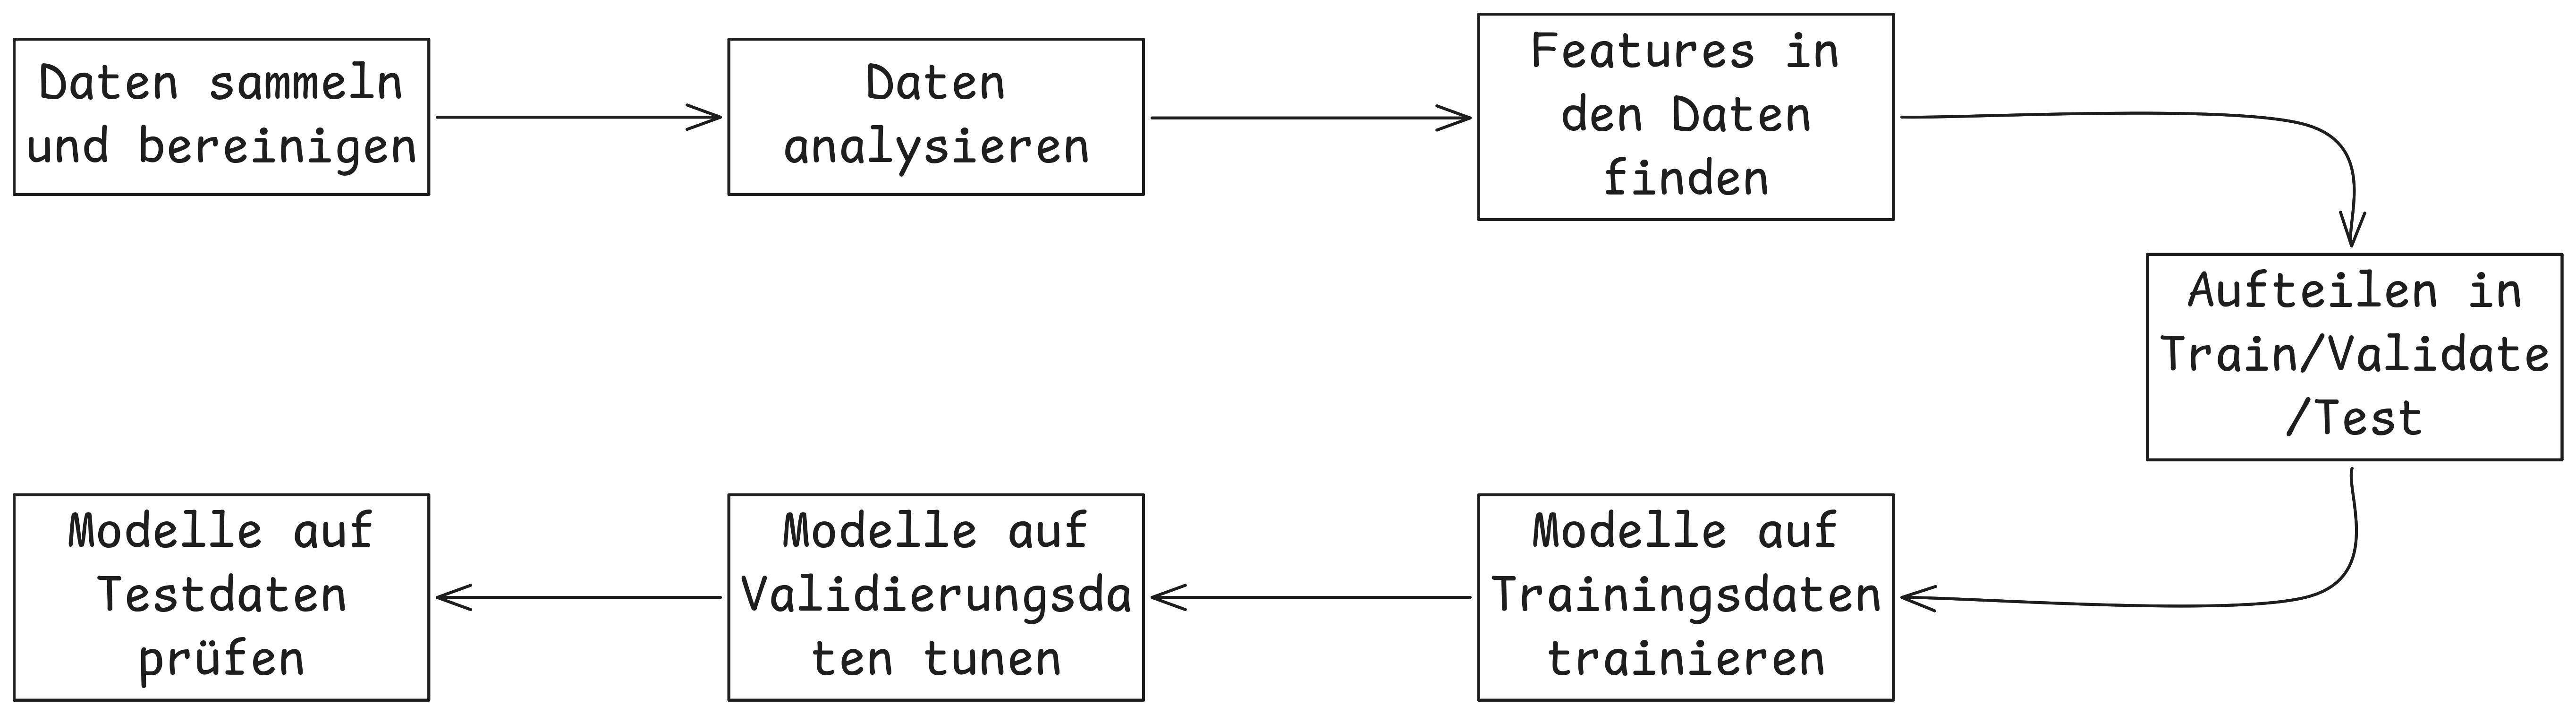
\includegraphics[width=0.9\linewidth]{./img/model_pipeline.png}
	\caption{Machinelerning Modell Pipeline}
    \label{fig:verticalcell}
\end{figure}

\begin{itemize}
    \item Zuerst müssen möglichst viele Relevante Datensätzen gesammelt werden.
	    Dazu gehöhren natürlich historische Aluminium Preis Daten, aber auch historische Preisdaten anderer Metalle.
		Auch Daten die die Wirtschaftliche gesamtlage abbilden, wie bespielsweise der S\&P 500 können relevant sein und werden in die Datenbasis mit aufgenommen.
	\item Diese Daten müssen daraufhin analysiert und bereinigt werden.
		Für eien erste analyse werden sie geplottet und visuel ausgewertet.
		Dabei können vielleicht schon erste Besonderheiten auffallen.
	
	\item im nächsten Schritt werden die Daten dann Maschinell analysiert und Markannte Verknüpfungen (sogenannte Features) unter den Daten können gefunden werden.


	\item um das Vorhersage Modell am Ende auch auf Korrekheit überprüfen zu können werden die Daten in 3 Teile aufgeteilt

	\begin{itemize}
		\item Trainings Daten werden genutzt um das Modell zu Trainieren
		\item Valididerungs Daten werden genutzt um Hyperparamenter des Modells feinzujustieren
		\item Test Daten werden genutzt um das Modell final auf Korrekheit zu überprüfen.
	\end{itemize}

	\item Die daten sind nun vorbereitet und verschiedene Modelle könen trainiert und miteinander verglichen werden.
\end{itemize}


TODO: Aluminium preis historisch Plotten

\pagebreak
\section{Regelbasierter Ansatz}
\begin{itemize}
    \item Umfang: ca. 2--3 Seiten
    \item Definition der Regeln
    \item Regeltypen:
    \begin{itemize}
        \item Trendregeln
        \item Volatilitätsregeln
        \item Schwellenregeln
    \end{itemize}
    \item Motivation jeder Regel
    \item Beispiele für Regelentscheidungen
\end{itemize}
\pagebreak
\section{KI-Komponente und Hybrid-Ansatz}
\begin{itemize}
    \item Umfang: ca. 2 Seiten
    \item Rolle der KI im System
    \item Begründung, warum KI nicht allein entscheidet
    \item Beschreibung der Hybrid-Logik
    \item Abgrenzung:
    \begin{itemize}
        \item Regel: deterministisch
        \item KI: Unterstützung bei Unsicherheit
    \end{itemize}
\end{itemize}
\pagebreak
\section{Ergebnisse und Evaluation}
\begin{itemize}
    \item Umfang: ca. 1,5--2 Seiten
    \item Testergebnisse auf dem Datensatz
    \item Metriken (wo sinnvoll)
    \item Beispielentscheidungen
    \item Vergleich:
    \begin{itemize}
        \item Regelbasierter Ansatz
        \item Hybrid-Ansatz
    \end{itemize}
\end{itemize}
\pagebreak
\section{Explainability und Entscheidungsnachvollziehbarkeit}
\begin{itemize}
    \item Umfang: ca. 1 Seite
    \item Erklärung der Entscheidungen
    \item Bereitgestellte Informationen für den Menschen
    \item Beispiel einer erklärten Entscheidung
\end{itemize}
\pagebreak
\section{Diskussion und Reflexion}
\label{sec:diskussion}

Die Diskussion und Reflexion der Ergebnisse zeigt, dass die Prognose des Aluminiumpreises eine herausfordernde Aufgabe darstellt, die durch hohe Volatilität und die Vielzahl von Einflussfaktoren geprägt ist. Die Messungen deuten darauf hin, dass das entwickelte System zwar in der Lage ist, gewisse Muster zu erkennen, jedoch die Vorhersagbarkeit über den 1-Tages-Horizont hinaus stark abnimmt.

\paragraph{Markteffizienz und Vorhersagbarkeit}
Das geringe Bestimmtheitsmaß ($R^2 \approx 0,0043$) und eine Richtungsgenauigkeit von $51,1 \%$ stehen im Einklang mit der \emph{Efficient Market Hypothesis} (EMH). Nach dieser Theorie spiegeln Marktpreise alle öffentlich verfügbaren Informationen wider, sodass Preisänderungen auf neue, unvorhersehbare Informationen reagieren und somit der Wahrscheinlichkeitstheorie (Random Walk) folgen. Die Ergebnisse deuten darauf hin, dass die historischen Preis- und Volumendaten allein nicht ausreichen, um systematische Vorhersagemuster zu extrahieren. Dies könnte auf die hohe Komplexität des Marktes zurückzuführen sein, in dem zahlreiche Faktoren (z. B. geopolitische Ereignisse, technologische Entwicklungen) eine Rolle spielen, die nicht direkt in den Zeitreihen erfasst werden.

\paragraph{Bedeutung der probabilistischen Prognose}
Ein Aspekt des Systems ist die Abkehr von algorithmischen Punktvorhersagen hin zu probabilistischen Verteilungen. Mittels MC-Dropout wird die Modellunsicherheit erkannt. Die Coverage von $90,8 \%$ für den 1-Tages-Horizont zeigt, dass das Modell in der Lage ist, die Varianz der Daten in einem statistischen Rahmen abzubilden. Dieser Ansatz bietet eine Grundlage für das Risikomanagement, da er keine exakte Punktlandung verspricht, sondern ein Spektrum der wahrscheinlichen Preisentwicklungen definiert. In Phasen mit hoher Unsicherheit (weite Konfidenzintervalle) kann die Beschaffungsstrategie  angepasst werden, um Risiken zu minimieren.

\paragraph{Grenzen der Datenbasis}
Die Beschränkung auf historische Preis- und Volumenzeitreihen sowie gesamtwirtschaftliche Indizes lässt weitere Faktoren außer Acht. Variablen wie physische Lagerbestände (z. B. LME Stocks), Energiepreise als Primärkostenfaktor der Produktion sowie politische Entscheidungen fließen nur indirekt über die Preisbildung in das Modell ein. Eine Erweiterung der Datenbasis um diese Zeitreihen oder unstrukturierte Daten (Text-Mining von Marktberichten) bietet Potenzial für eine Steigerung der Signalqualität.

\pagebreak
\section{Fazit und Ausblick}
\begin{itemize}
    \item Umfang: ca. 0,5--1 Seite
    \item Zusammenfassung der Ergebnisse
    \item Nutzen des Ansatzes
    \item Mögliche Erweiterungen:
    \begin{itemize}
        \item weitere Daten
        \item Regelverfeinerung
    \end{itemize}
\end{itemize}
\pagebreak
\section{Anhang}
\begin{itemize}
    \item Umfang: optional
    \item Code-Ausschnitte
    \item Zusätzliche Diagramme
    \item Vollständige Regeldefinitionen
    \item Beispieldatensätze
\end{itemize}
\pagebreak

\printbibliography[title={Literaturverzeichnis}]

%\pagebreak
%\rhead{Ehrenwörtliche Erklärung}

\phantomsection \label{Ehrenwörtliche Erklärung}
\pagenumbering{gobble}% Seitennummerierungsstil ganz ohne Ausgabe der Nummern verwenden!
\addcontentsline{toc}{section}{Ehrenwörtliche Erklärung} %Anhang ohne Nummer
%\section*{Ehrenwörtliche Erklärung}
\renewcommand{\thesection}{\Roman{section}}

\begin{singlespacing} 
    \textsf{\begin{minipage}{.4\textwidth} %Einbinden des Logos mit rechtsbündiger Ausrichtung. Weitere Logos im Bilderordner verfügbar.
            \begin{flushleft}
                
\includegraphics[width=1.5\textwidth]{Bilder/OTH_Regensburg_Logo_3line_pos_bg}\\
            \end{flushleft}
        \end{minipage}
    }
\end{singlespacing} 
    % Zeilenabstand
    \onehalfspacing	
    
    %Beschriftung der Titelseite
    \begin{center}
        \vspace*{2 cm} %3 cm Vorspann
        \Large
        \textbf{ERKLÄRUNG \\ZUR MASTERARBEIT VON}
    \end{center}
        
	 \vspace*{1 cm} 
        \normalsize
        
	 \begin{table}[H]
        \begin{tabular}{ll}
        Name: & N a m e \\
        Vorname: & V o r n a m e \\
        Studiengang: & Informatik (M.Sc.)
        \end{tabular}
    \end{table}
    
     \vspace*{1 cm} 
        \normalsize
    

    \begin{enumerate}
        \item Mir ist bekannt, dass dieses Exemplar der Masterarbeit als Prüfungsleistung in das Eigentum der Ostbayerischen Technischen Hochschule Regensburg übergeht.\\
        
        \item Ich erkläre hiermit, dass ich diese Masterarbeit selbständig verfasst, noch nicht anderweitig für Prüfungszwecke vorgelegt, keine anderen als die angegebenen Quellen und Hilfsmittel benutzt sowie wörtliche und sinngemäße Zitate als solche gekennzeichnet habe. 
    \end{enumerate}


     \vspace*{3 cm} 
        \normalsize
        
    
    Regensburg, den TT.MM.JJJJ\\ \\
....................................................\\
Unterschrift

\end{document}
